\chapter{Lie Groups and Lie Algebras}
\section{Lie groups}
\subsection{Lie groups and homomorphisms}
A \textbf{Lie group} is a smooth manifold $G$ (without boundary) that is also a group in the algebraic sense, with the property that the multiplication map $m:G\times G\to G$ and inversion map $i:G\to G$, given by
\[m(g,h)=gh,\quad i(g)=g^{-1}\]
are both smooth. A Lie group is, in particular, a topological group. \par
The group operation in an arbitrary Lie group is denoted by juxtaposition, except in certain abelian groups such as Rn in which the operation is usually written additively. It is traditional to denote the identity element of an arbitrary Lie group by the symbol $e$.\par
The following alternative characterization of the smoothness condition is sometimes useful.
\begin{proposition}
If $G$ is a smooth manifold with a group structure such that the map $G\times G\to G$ given by $(g,h)\mapsto gh^{-1}$ is smooth, then $G$ is a Lie group.
\end{proposition}
\begin{proof}
Let we denote this map by $\sigma$. We have
\[i(g)=\sigma(e,g),\quad m(g,h)=\sigma(g,i(h)).\]
Thus if $\sigma$ is smooth, so is $i$, and hence $m$.
\end{proof}
If $G$ is a Lie group, any element $g\in G$ defines maps $L_g,R_g:G\to G$, called \textbf{left translation} and \textbf{right translation}, respectively, by
\[L_g(h)=gh,\quad R_g(h)=hg.\]
Because $L_g$ can be expressed as the composition of smooth maps
\[\begin{tikzcd}
G\ar[r,"\iota_g"]&G\times G\ar[r,"m"]&G
\end{tikzcd}\]
where $\iota_g(h)=(g,h)$ and $m$ is multiplication, it follows that $L_g$ is smooth. It is actually a diffeomorphism of $G$, because $L_{g^{-1}}$ is a smooth inverse for it. Similarly,
$R_g:G\to G$ is a diffeomorphism.
\begin{example}[\textbf{Lie Groups}]
Each of the following manifolds is a Lie group with the indicated group operation.
\begin{itemize}
\item[(a)] The general linear group $\GL_n(\R)$ is the set of invertible $n\times n$ matrices with real entries. It is a group under matrix multiplication, and it is an open submanifold of the vector space $\mathcal{M}_n(\R)$. Multiplication is smooth because the matrix entries of a product matrix $AB$ are polynomials in the entries of $A$ and $B$. Inversion is smooth by Cramer's rule.
\item[(b)] Let $\GL^+_n(\R)$ denote the subset of $\GL_n(\R)$ consisting of matrices with positive determinant. Because $\det(AB)=(\det A)(\det B)$ and $\det A^{-1}=(\det A)^{-1}$, it is a subgroup of $\GL_n(\R)$ and because it is the preimage of $(0,\infty)$ under the continuous determinant function, it is an open subset of $\GL_n(\R)$ and therefore an $n^2$-dimensional manifold. The group operations are the restrictions of those of $\GL_n(\R)$ so they are smooth. Thus $\GL^+_n(\R)$ is a Lie group.
\item[(c)] Suppose $G$ is an arbitrary Lie group and $H\sub G$ is an open subgroup $($a subgroup that is also an open subset$)$. By the same argument as in part (b), $H$ is a Lie group with the inherited group structure and smooth manifold structure.
\item[(d)] The \textbf{complex general linear group} $\GL_n(\C)$ is the group of invertible complex $n\times n$ matrices under matrix multiplication. It is an open submanifold of $\mathcal{M}_n(\C)$ and thus a $2n^2$-dimensional smooth manifold, and it is a Lie group because matrix products and inverses are smooth functions of the real and imaginary parts of the matrix entries.
\item[(e)] If $V$ is any real or complex vector space, $\GL(V)$ denotes the set of invertible linear maps from $V$ to itself. It is a group under composition. If $V$ has finite dimension $n$, any basis for $V$ determines an isomorphism of $\GL(V)$ with $\GL_n(\R)$ or $\GL_n(\C)$, so $\GL(V)$ is a Lie group. The transition map between any two such isomorphisms is given by a map of the form $A\mapsto B^{-1}AB$ $($where $B$ is the transition matrix between the two bases$)$, which is smooth. Thus, the smooth manifold structure on $\GL(V)$ is independent of the choice of basis.
\item[(f)] The real number field $\R$ and Euclidean space $\R^n$ are Lie groups under addition, because the coordinates of $x-y$ are smooth. Similarly, $\C$ and $\C^n$ are Lie groups under addition.
\item[(g)] The set $\R^*$ of nonzero real numbers is a $1$-dimensional Lie group under multiplication. In fact, it is exactly $\GL_1(\R)$ if we identify a $1\times 1$ matrix with the corresponding real number.) The subset $\R^+$ of positive real numbers is an open subgroup, and is thus itself a $1$-dimensional Lie group. The set $\C^*$ of nonzero complex numbers is a $2$-dimensional Lie group under complex multiplication, which can be identified with $\GL_1(\C)$.
\item[(h)] The circle $S^1\sub\C^*$ is a smooth manifold and a group under complex multiplication. With appropriate angle functions as local coordinates on open subsets of $S^1$, multiplication and inversion have the smooth coordinate expressions $(\theta_1,\theta_2)\mapsto\theta_1+\theta_2$ and $\theta_1\mapsto-\theta$, and therefore $S^1$ is a Lie group, called the \textbf{circle group}.
\item[(i)] Given Lie groups $G_1,\dots,G_k$, their direct product is the product manifold
$G_1\times\cdots\times G_k$ with the group structure given by componentwise multiplication:
\[(g_1,\dots,g_k)(g_1',\dots,g_k')=(g_1g_1',\dots,g_kg_k')\]
It is a Lie group. For example, the $n$-torus $T^n=S^1\times\cdots\times S^1$ is an $n$-dimensional abelian Lie group.
\item[(j)] Any group with the discrete topology is a topological group, called a \textbf{discrete group}. If in addition the group is finite or countably infinite, then it is a zero-dimensional Lie group, called a \textbf{discrete Lie group}.
\end{itemize}
\end{example}
Now we consider maps between Lie groups. If $G$ and $H$ are Lie groups, a \textbf{Lie group homomorphism} from $G$ to $H$ is a smooth map $F:G\to H$ that is also a group homomorphism. It is called a \textbf{Lie group isomorphism} if it is also a diffeomorphism, which implies that it has an inverse that is also a Lie group homomorphism. In this case we say that $G$ and $H$ are \textbf{isomorphic Lie groups}.
\begin{example}[\textbf{Lie Group Homomorphisms}]
\mbox{}
\begin{itemize}
\item[(a)] The inclusion map $S^1\hookrightarrow\C^*$ is a Lie group homomorphism.
\item[(b)] Considering $\R$ as a Lie group under addition, and $\R^*$ as a Lie group under multiplication, the map $\exp:\R\to\R^*$ is smooth, and is a Lie group homomorphism. The image of $\exp$ is the open subgroup $\R^+$ consisting of positive real numbers, and $\exp:\R\to\R^+$ is a Lie group isomorphism with inverse $\log:\R^+\to\R$. Similarly, $\exp:\C\to\C^*$ is a Lie group homomorphism. It is surjective but not injective, because its kernel is $2\pi i\Z$.
\item[(c)] The map $\eps:\R\to S^1$ defined by $\eps(x)=e^{2\pi ix}$ is a Lie group homomorphism whose kernel is the set $\Z$ of integers. Similarly, the map $\eps^n:\R^n\to T^n$ defined by $\eps^n(x_1,\dots,x^n)=(e^{2\pi ix^1},\dots,e^{2\pi ix^n})$ is a Lie group homomorphism whose kernel is $\Z^n$.
\item[(d)] The determinant function $\det:\GL_n(\R)\to\R^*$ is smooth because $\det A$ is a polynomial in the matrix entries of $A$. It is a Lie group homomorphism
because $\det(AB)=(\det A)(\det B)$. Similarly, $\det:\GL_n(\C)\to\C^*$ is a Lie group homomorphism.
\item[(e)] If $G$ is a Lie group and $g\in G$, conjugation by $g$ is the map $C_g:G\to G$ given by $C_g(h)=ghg^{-1}$. Because group multiplication and inversion are smooth, $C_g$ is smooth, and a simple computation shows that it is a group homomorphism. In fact, it is an isomorphism, because it has $C_{g^{-1}}$ as an inverse. A subgroup $H\sub G$ is said to be normal if $C_g(H)=H$ for every $g\in G$.
\end{itemize}
\end{example}
The next theorem is important for understanding many of the properties of Lie group homomorphisms.
\begin{theorem}\label{Lie homo constant rank}
Every Lie group homomorphism has constant rank.
\end{theorem}
\begin{proof}
Let $F:G\to H$ be a Lie group homomorphism, and let $e_G$ and $e_H$ denote the identity elements of $G$ and $H$, respectively. Suppose $g_0$ is an arbitrary element of $G$. We will show that $dF_{g_0}$ has the same rank as $dF_{e_G}$. The fact that $F$ is a homomorphism means that for all $g\in G$,
\[F(L_{g_0}(g))=F(g_0g)=F(g_0)F(g)=L_{F(g_0)}F(g)\]
or in other words, the following diagram commutes:
\[\begin{tikzcd}
G\ar[r,"F"]\ar[d,swap,"L_{g_0}"]&H\ar[d,"L_{F(g_0)}"]\\
G\ar[r,"F"]&H
\end{tikzcd}\] 
Taking differentials of both sides at the identity and using Proposition~\ref{differential mani prop}(b), we find that
\[dF_{g_0}\circ d(L_{g_0})_{e_G}=d(L_{F(g_0)})_{e_H}\circ dF_{e_H}\]
Left multiplication by any element of a Lie group is a diffeomorphism, so both $d(L_{g_0})_{e_G}$ and $d(L_{F(g_0)})_{e_H}$ are isomorphisms. Because composing with an isomorphism does not change the rank of a linear map, it follows that $dF_{g_0}$ and $dF_{e_G}$ have the same rank.
\end{proof}
\begin{corollary}\label{Lie isomorphism iff}
A Lie group homomorphism is a Lie group isomorphism if and only if it is bijective.
\end{corollary}
\begin{proof}
The global rank theorem shows that a bijective Lie group homomorphism is a diffeomorphism.
\end{proof}
\subsection{The universal covering group}
Covering space theory yields the following important result about Lie groups.
\begin{theorem}[\textbf{Universal Covering Group}]\label{Lie universal covering group}
Let $G$ be a connected Lie group. Then there exists a simply connected Lie group $\widetilde{G}$, called the \textbf{universal covering group} of $G$, that admits a smooth covering map $\pi:\widetilde{G}\to G$ that is also a Lie group homomorphism with kernel isomorphic to $\pi_1(G)$ and is a discrete central group in $\widetilde{G}$.
\end{theorem}
\begin{proof}
Let $\widetilde{G}$ be the universal covering manifold of $G$ and $\pi:\widetilde{G}\to G$ be the corresponding smooth covering map. Then $\pi\times\pi:\widetilde{G}\times\widetilde{G}\to G\times G$ is also a smooth covering map.\par
Let $m:G\times G\to G$ and $i:G\to G$ denote the multiplication and inversion maps of $G$, respectively, and let $\widetilde{e}$ be an arbitrary element of the fiber $\pi^{-1}(e)$. Since $\widetilde{G}$ is simply connected, the lifting criterion for covering maps guarantees that the map $m\circ(\pi\times \pi):\widetilde{G}\times\widetilde{G}\to G$ has a unique continuous lift $\widetilde{m}:\widetilde{G}\times\widetilde{G}\to\widetilde{G}$ satisfying $\widetilde{m}(\widetilde{e},\widetilde{e})=\widetilde{e}$ and $\pi\circ\widetilde{m}=m\circ(\pi\times\pi)$:
\[\begin{tikzcd}
\widetilde{G}\times\widetilde{G}\ar[r,"\widetilde{m}"]\ar[d,swap,"\pi\circ\pi"]&\widetilde{G}\ar[d,"\pi"]\\
G\times G\ar[r,"m"]&G
\end{tikzcd}\]
Because $\pi$ is a surjective local diffeomorphism and $\pi\circ\widetilde{m}$ is smooth, it follows from Proposition~\ref{smooth iff composition smooth}(b) that $\widetilde{m}$ is smooth. By the same reasoning, $i\circ\pi:\widetilde{G}\to G$ has a smooth lift $\widetilde{i}$ such that $\widetilde{i}(\widetilde{e})=\widetilde{e}$ and $\pi\circ\widetilde{i}=i\circ\pi$:
\[\begin{tikzcd}
\widetilde{G}\ar[r,"\widetilde{i}"]\ar[d,swap,"\pi"]&\widetilde{G}\ar[d,"\pi"]\\
G\ar[r,"i"]&G
\end{tikzcd}\]
We define multiplication and inversion in $\widetilde{G}$ to be $\widetilde{m}$ and $\widetilde{i}$. Then from the commutative diagrams we have
\begin{align}\label{universal cover group-1}
\pi(x,y)=\pi(x)\pi(y),\quad\pi(x^{-1})\pi(x)^{-1}.
\end{align}
It remains only to show that $\widetilde{G}$ is a group with these operations, for then it is a Lie group because $\widetilde{m}$ and $\widetilde{i}$ are smooth, and $(\ref{universal cover group-1})$ shows that $\pi$ is a homomorphism.\par
First we show that $\widetilde{e}$ is an identity for multiplication in $\widetilde{e}$. Consider the map $f:\widetilde{G}\to\widetilde{G}$ defined by $f(x)=\widetilde{e}x$. Then $(\ref{universal cover group-1})$ implies that 
\[\pi\circ f(x)=\pi(\widetilde{e}x)=\pi(\widetilde{e})\pi(x)=e\pi(x)=\pi(x)\]
so $f$ is a lift of $\pi:\widetilde{G}\to G$. Since the identity map $\mathrm{id}_{\widetilde{G}}$ is already a lift of $\pi$, and it agrees with $f$ at a point because $f(\widetilde{e})=\widetilde{m}(\widetilde{e},\widetilde{e})=\widetilde{e}$, the unique lifting property of covering maps implies that $f=\mathrm{id}_{\widetilde{G}}$, or equivalently, $\widetilde{e}x=x$ for all $x$ in $\widetilde{G}$. The same argument shows that $x\widetilde{e}=x$.\par
Next, to show that multiplication in $\widetilde{G}$ is associative, consider the two maps $\alpha_L,\alpha_R:\widetilde{G}\times\widetilde{G}\times\widetilde{G}\to\widetilde{G}$ defined by
\[\alpha_L(x,y,z)=(xy)z,\quad\alpha_R(x,y,z)=x(yz)\]
Then $(\ref{universal cover group-1})$ applied repeatedly implies that
\[\pi\circ\alpha_L(x,y,z)=(\pi(x)\pi(y))\pi(z)=\pi(x)(\pi(y)\pi(z))=\pi\circ\alpha_R(x,y,z)\]
so $\alpha_L$ and $\alpha_R$ are both lifts of the same map $\alpha(x,y,z)=\pi(x)\pi(y)\pi(z)$. Because $\alpha_L$ and $\alpha_R$ agree at $(\widetilde{e},\widetilde{e},\widetilde{e})$, they are equal.\par
Finally, let $x_0\in\widetilde{G}$. To show $x_0x_0^{-1}=x_0^{-1}x_0=\widetilde{e}$ we define a map $g:\widetilde{G}\to\widetilde{G}$ by $g(x)=x_0^{-1}x_0x$. With the same argument we can show that $g$ is a lift of $\pi$, thus equal to $\mathrm{id}_{\widetilde{G}}$. Hence we claim $x_0^{-1}x_0=\widetilde{e}$, and similarly $x_0x_0^{-1}=\widetilde{e}$, so $\widetilde{G}$ is a group.\par
Let $\varphi\in\Aut_{\pi}(\widetilde{G})$, we consider the map $\widetilde{\varphi}:g\mapsto\varphi(\widetilde{e})g$. We have
\[\pi\circ\widetilde{\varphi}(g)=\pi(\varphi(\widetilde{e})g)=e\cdot\pi(g)=\pi(g),\]
so $\widetilde{\varphi}$ is a lifting of $\pi:\widetilde{G}\to G$. Since $\varphi$ is also a lifting of $\pi:\widetilde{G}\to G$ and $\varphi(\widetilde{e})=\widetilde{\varphi}(\widetilde{e})$, we conclude that $\varphi=\widetilde{\varphi}$. With this observation, we define a map
\[\mathrm{ev}:\Aut_{\pi}(\widetilde{G})\to\ker\pi,\quad \varphi\mapsto\varphi(\widetilde{e}).\]
Then $\mathrm{ev}$ is a homomorphism because
\[\mathrm{ev}(\varphi\circ\psi)=(\varphi\circ\psi(\widetilde{e}))=\varphi(\psi(\widetilde{e}))=\varphi(\widetilde{e})\cdot\psi(\widetilde{e})=\mathrm{ev}(\varphi)\cdot\mathrm{ev}(\psi).\]
Since $\ker\pi$ has the same cardinality as $\Aut_{\pi}(\widetilde{G})$, we conclude that $\Aut_{\pi}(\widetilde{G})$ is isomorphic to $\Aut_{\pi}(\widetilde{G})$, and hence to $\pi_1(G)$, as groups. The group $\ker\pi$ is central because it is a discrete normal subgroup of a connected group. 
\end{proof}
\begin{theorem}
Let $G$ be a connected Lie group. Then the universal covering group of $G$ is unique in the following sense: if $\widetilde{G}$ and $\widetilde{G}'$ are simply connected Lie groups that admit smooth covering maps $\pi:\widetilde{G}\to G$ and $\pi':\widetilde{G}'\to G$ that are also Lie group homomorphisms, then there exists a Lie group isomorphism $\varPhi:\widetilde{G}\to\widetilde{G}'$ such that $\pi'\circ\varPhi=\pi$.
\end{theorem}
\begin{proof}
Assume that $\widetilde{G}$ and $\widetilde{G}'$ are universal covering groups of $G$. Since the universal covering manifold is unique, there exists a diffeomorphism $\varPhi:\widetilde{G}\to\widetilde{G}'$ such that $\pi'\circ\varPhi=\pi$ and $\varPhi(e_{\widetilde{G}})=e_{\widetilde{G}'}$. Now we only need to show $\varPhi$ is a homomorphism, which means \[\varPhi\circ\widetilde{m}=\widetilde{m}'\circ(\varPhi\times\varPhi),\]
where $\widetilde{m}$ and $\widetilde{m}'$ are the multiplication maps in $\widetilde{G}$ and $\widetilde{G}'$, respectively. It is clear that both $\varPhi\circ\widetilde{m}$ and $\widetilde{m}'\circ(\varPhi\times\varPhi)$ are lifts of the same map $m\circ(\pi\times\pi)$, where $m$ is the multiplication map of $G$. Moreover, these two maps agree on $(\widetilde{e},\widetilde{e})$. Therefore by the uniqueness of liftings we get the require result.
\end{proof}
\subsection{Lie subgroups}
Suppose $G$ is a Lie group. A \textbf{Lie subgroup} of $G$ is a subgroup of $G$ endowed with a topology and smooth structure making it into a Lie group and an immersed submanifold of $G$. The following proposition shows that embedded subgroups are automatically Lie subgroups.
\begin{proposition}\label{Lie subgroup embedd mani}
Let $G$ be a Lie group, and suppose $H\sub G$ is a subgroup that is also an embedded submanifold. Then $H$ is a Lie subgroup.
\end{proposition}
\begin{proof}
We need only check that multiplication $H\times H\to H$ and inversion $H\to H$ are smooth maps. Because multiplication is a smooth map from $G\times G$ into $G$, its
restriction is clearly smooth from $H\times H$ into $G$ (this is true even if $H$ is merely immersed). Because $H$ is a subgroup, multiplication takes $H\times H$ into $H$, and since $H$ is embedded, this is a smooth map into $H$ by Corollary~\ref{resrtict codomain to embedd}. A similar argument applies to inversion. This proves that $H$ is a Lie subgroup.
\end{proof}
The simplest examples of embedded Lie subgroups are the open subgroups. The
following lemma shows that the possibilities for open subgroups are limited.
\begin{lemma}\label{Lie subgroup open}
Suppose $G$ is a Lie group and $H\sub G$ is an open subgroup. Then $H$ is an embedded Lie subgroup. In addition, $H$ is closed, so it is a union of connected components of $G$.
\end{lemma}
\begin{proof}
If $H$ is open in $G$, then it is embedded by Proposition~\ref{open submani iff}. By Proposition~\ref{topo group prop} $H$ is both open and closed, so it is a union of components.
\end{proof}
If $G$ is a Lie group, the connected component of $G$ containing the identity is called the \textbf{identity component} of $G$ and denoted by $G_0$.
\begin{proposition}\label{Lie identity component}
Let $G$ be a Lie group and let $G_0$ be its identity component. Then $G_0$ is a normal subgroup of $G$, and is the only connected open subgroup. Every
connected component of $G$ is diffeomorphic to $G_0$.
\end{proposition}
\begin{proof}
Since $G_0$ is connected, it gengerates a connected open subgroup $H$ of $G$. But $G_0$ is a connected component contained in $H$, so it follows that $H=G_0$.\par 
Let $g\in G$ be an arbitrary element, and consider the subgroup $gG_0g^{-1}=L_g\circ R_{g^{-1}}(G_0)$. Since $L_g$ and $R_{g^{-1}}$ are both diffeomorphisms, it 
follows that $gG_0g^{-1}$ is an open connected subgroup containing the identity. Since $G_0$ is a connected component, it follows that $gG_0g^{-1}\sub G_0$, thus 
they must equal. This shows $G_0$ is normal.\par 
Let $H$ be a connected open subgroup. Then $H$ contains the identity, hence  is contained in $G_0$. Moreover, by Lemma~\ref{Lie subgroup open} $H$ is also closed, 
therefore by the connectness of $G_0$ we get $H=G_0$, which means $G_0$ is the only open connected subgroup.\par
Now let $C$ be a connected component of $G$, and choose a element $g\in C$. Then $L_{g^{-1}}(C)$is a connected open subset containing the identity, thus is contained 
in $G_0$. Since the same argument gives $L_g(G_0)\sub C$, we conclude $L_g(G_0)=C$.
\end{proof}
Now we move beyond the open subgroups to more general Lie subgroups. The
following proposition shows how to produce many more examples of embedded Lie
subgroups.
\begin{proposition}\label{Lie homo ker}
Let $F:G\to H$ be a Lie group homomorphism. The kernel of $F$ is a properly embedded Lie subgroup of $G$, whose codimension is equal to the rank of $F$.
\end{proposition}
\begin{proof}
Because $F$ has constant rank, its kernel $F^{-1}(e)$ is a properly embedded
submanifold of codimension equal to $\rank F$. It is thus a Lie subgroup by Proposition~\ref{Lie subgroup embedd mani}.
\end{proof}
Complementary to the preceding result about kernels is the following result about images.
\begin{proposition}\label{Lie homo injective}
If $F:G\to H$ is an injective Lie group homomorphism, the image of $F$ has a unique smooth manifold structure such that $F(G)$ is a Lie subgroup of $H$ and $F:G\to F(G)$ is a Lie group isomorphism.
\end{proposition}
\begin{proof}
Since a Lie group homomorphism has constant rank, it follows from the global rank theorem that $F$ is a smooth immersion. Proposition~\ref{image immersion submani} shows that $F(G)$ has a unique smooth manifold structure such that it is an immersed submanifold of $H$ and $F$ is a diffeomorphism onto its image. It is a Lie group (because $G$ is), and it is a subgroup for algebraic reasons, so it is a Lie subgroup. Because $F:G\to F(G)$ is a group isomorphism and a diffeomorphism, it is a Lie group isomorphism.
\end{proof}
\begin{example}[\textbf{Embedded Lie Subgroups}]\label{Lie subgroups eg}
\mbox{}
\begin{itemize}
\item[(a)] The subgroup $\GL^+_n(\R)\sub\GL_n(\R)$ is an open subgroup and thus an embedded Lie subgroup. It is indeed the identity component of $\GL_n(\R)$.
\item[(b)] The circle $S^1$ is an embedded Lie subgroup of $\C^*$ because it is a subgroup and an embedded submanifold.
\item[(c)] The set $\SL_n(\R)$ of $n\times n$ real matrices with determinant equal to $1$ is called the \textbf{special linear group} of degree $n$. Because $\SL_n(\R)$ is the kernel of the Lie group homomorphism $\det:\GL_n(\R)\to\R^*$, it is a properly embedded Lie subgroup. Because the determinant function is surjective, it is a smooth submersion by the global rank theorem, so $\SL_n(\R)$ has dimension $n^2-1$.
\item[(d)] Let $n$ be a positive integer, and define a map $\beta:\GL_n(\C)\to\GL_{2n}(\R)$ by replacing each complex matrix entry $a+ib$ with the $2\times 2$ block $(\begin{smallmatrix}
a&b\\
-b&a
\end{smallmatrix})$:
\[\beta\begin{pmatrix}
a^1_1+ib^1_1&\cdots&a^1_n+ib^1_n\\
\vdots&&\vdots\\
a^n_1+ib^n_1&\cdots&a^n_n+ib^n_n
\end{pmatrix}
=\begin{pmatrix}
\begin{array}{cc}
a^1_1&-b^1_1\\
b^1_1&a^1_1
\end{array}&\cdots&\begin{array}{cc}
a^1_n&-b^1_n\\
b^1_n&a^1_n
\end{array}\\
\vdots&&\vdots\\
\begin{array}{cc}
a^n_1&-b^n_1\\
b^n_1&a^n_1
\end{array}&\cdots&\begin{array}{cc}
a^n_n&-b^n_n\\
b^n_n&a^n_n
\end{array}
\end{pmatrix}
\]
It is straightforward to verify that $\beta$ is an injective Lie group homomorphism whose image is a properly embedded Lie subgroup of $\GL_{2n}(\R)$. Thus, $\GL_n(\C)$ is isomorphic to this Lie subgroup of $\GL_{2n}(\R)$.
\item[(e)] The subgroup $\SL_n(\C)\sub\GL_n(\C)$ consisting of complex matrices of determinant $1$ is called the \textbf{complex special linear group} of degree $n$. It is the kernel of the Lie group homomorphism $\det:\GL_n(\C)\to\C^*$. This homomorphism is surjective, so it is a smooth submersion by the global rank theorem. Therefore, $\SL_n(\C)=\ker\det$ is a properly embedded Lie subgroup whose dimension is $2n^2-2$.
\end{itemize}
\end{example}
Finally, here is an example of a Lie subgroup that is not embedded.
\begin{example}[\textbf{A Dense Lie Subgroup of the Torus}]
Let $H\sub T^2$ be the dense submanifold of the torus that is the image of the immersion $\gamma:\R\to T^2$ defined in Example~\ref{dense curve torus}. It is easy to check that $\beta$ is an injective Lie group homomorphism, and thus $H$ is an immersed Lie subgroup of $T^2$ by Proposition~\ref{Lie homo injective}.
\end{example}
In general, smooth submanifolds can be closed without being embedded (as is, for example, the figure-eight curve) or embedded without being closed (as is the open unit ball in $\R^n$). However, as the next theorem shows, Lie subgroups have the remarkable property that closedness and embeddedness are not independent. This means that every embedded Lie subgroup is properly embedded. 
\begin{theorem}\label{Lie subgroup closed iff embed}
Suppose $G$ is a Lie group and $H\sub G$ is a Lie subgroup. Then $H$ is closed in $G$ if and only if it is embedded.
\end{theorem}
\begin{figure}[htbp]
\centering
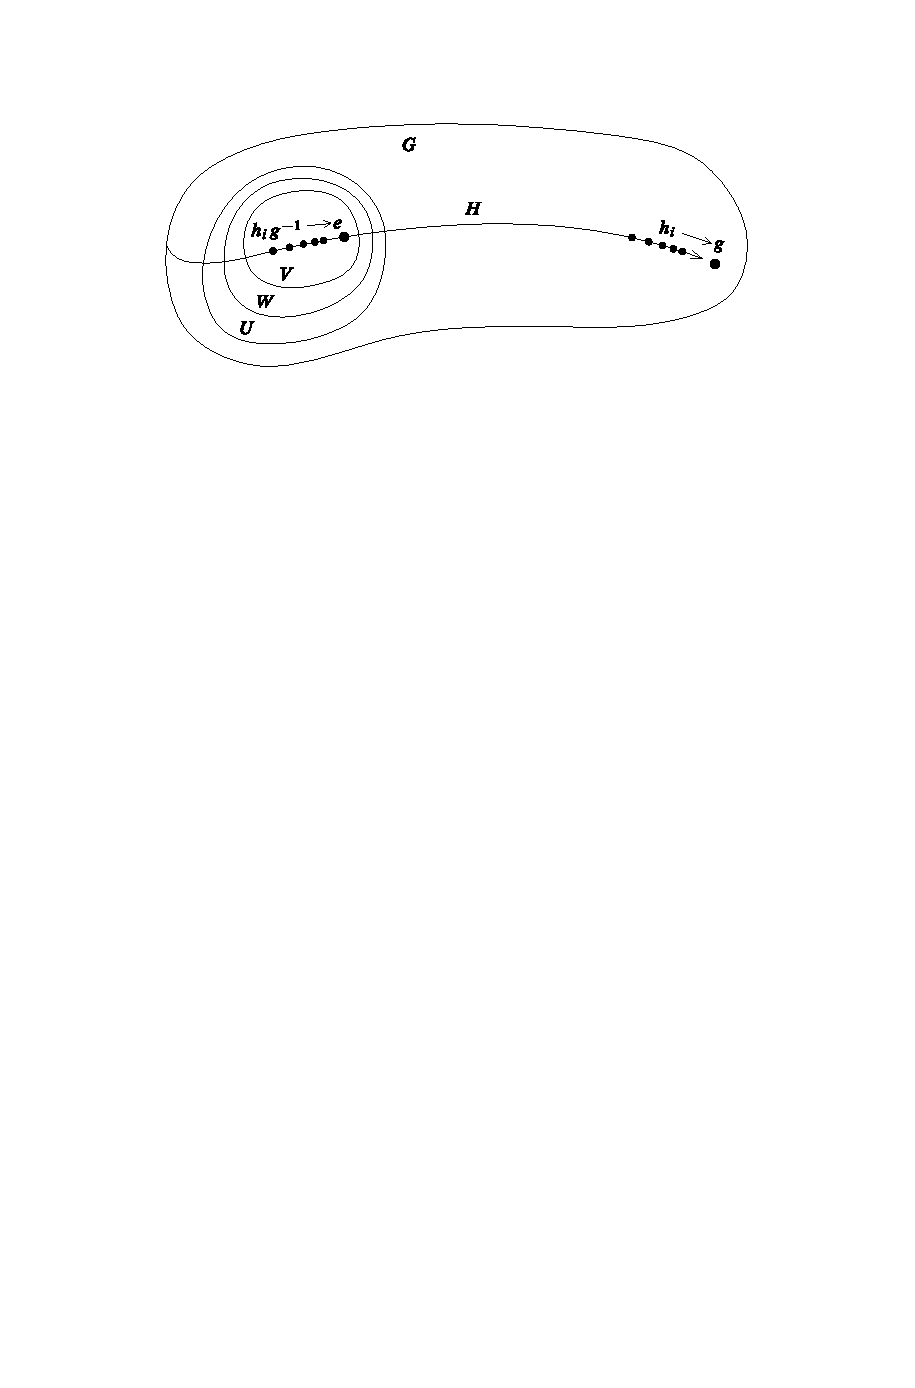
\includegraphics{pictures/Lie-closed-1}
\caption{An embedded Lie subgroup is closed.}
\end{figure}
\begin{proof}
Assume first that $H$ is embedded in $G$. To prove that $H$ is closed, let $g$ be an arbitrary point of $\widebar{H}$. Then there is a sequence $(h_i)$ of points in $H$ converging to $g$. Let $U$ be the domain of a slice chart for $H$ containing the identity, and let $W$ be a smaller neighborhood of $e$ such that $\widebar{W}\sub U$. By Lemma~\ref{topo group identity nbhd lem}, there is a neighborhood $V$ of $e$ with the property that $g_1g_2^{-1}\in W$ whenever $g_1,g_2\in V$.\par
Because $h_ig^{-1}\to e$, by discarding finitely many terms of the sequence we may assume that $h_ig^{-1}\in V$ for all $i$. This implies that
\[h_ih_j^{-1}=(h_ig^{-1})(h_jg^{-1})^{-1}\in W\]
for all $i$ and $j$. Fixing $j$ and letting $i\to\infty$, we find that $h_ih_j^{-1}\to gh_j^{-1}\in\widebar{W}\sub U$. Since $H\cap U$ is a slice, it is closed in $U$, and therefore $gh_j^{-1}\in H$, which implies $g\in H$. Thus $H$ is closed.\par
Conversely, assume $H$ is a closed Lie subgroup, and let $m=\dim H$ and $n=\dim G$. We need to show that $H$ is an embedded submanifold of $G$. If $m=n$, then $H$ is embedded by Proposition~\ref{open submani iff}, so we may assume henceforth that $m<n$.\par
It suffices to show that for some $h_1\in H$, there is a neighborhood $U_1$ of $h_1$ in $G$ such that $H\cap U_1$ is an embedded submanifold of $U_1$; for then if $h$ is any other point of $H$, right translation $R_{h_1^{-1}h}$ is a diffeomorphism of $G$ that takes $H$ to $H$, and takes $U_1$ to a neighborhood $U'_1$ of $h$ such that $H\cap U'_1$ is embedded in $U'_1$,
so it follows from the local slice criterion that $H$ is an embedded submanifold of $G$.\par
Because every immersed submanifold is locally embedded (Proposition~\ref{immerse local embedd}), there exist a neighborhood $V$ of $e$ in $H$ and a slice chart $(U,\varphi)$ for $V$ in $G$ centered at $e$. By shrinking $U$ if necessary, we may assume that it is a coordinate cube, and $U\cap V$ is the set of points whose coordinates are of the form $\{x^{m+1}=\cdots=x^n=0\}$. Let $S\sub U$ be the set of points with coordinates of the form $\{x^1=\cdots=x^m=0\}$; it is the slice perpendicular to $U\cap V$ in these coordinates. Then $S$ is an embedded submanifold of $U$ and hence of $G$. Note that in these coordinates, $T_eV$ is spanned by the first $m$ coordinate vectors and $T_eS$ by the last $n-m$, so $T_eG=T_eV\oplus T_eS$.
\begin{figure}[htbp]
\centering
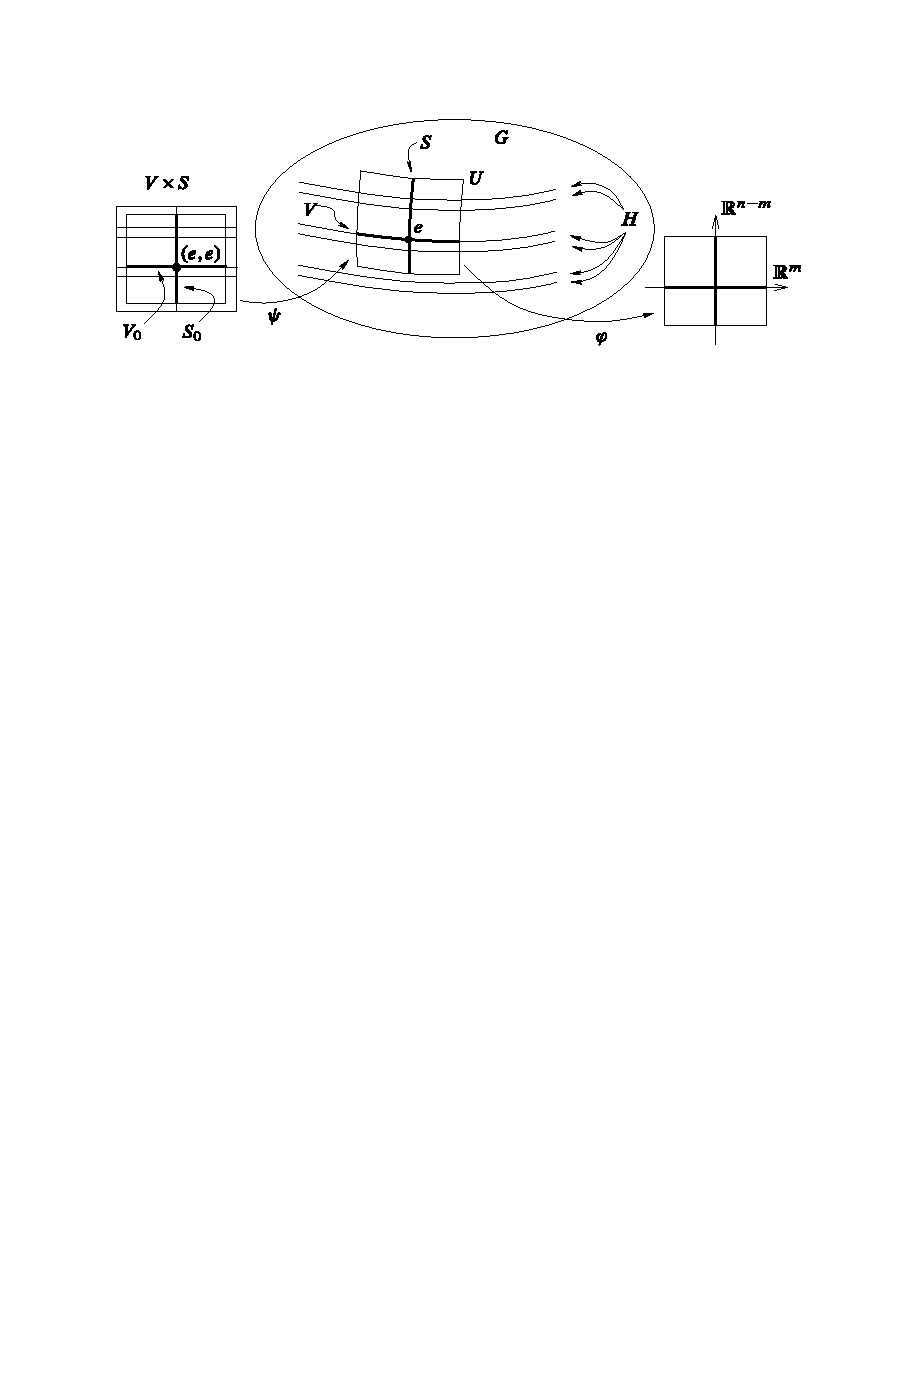
\includegraphics{pictures/Lie-closed-2}
\caption{Finding a slice chart.}
\end{figure}\par
Now consider the map $\psi:V\times S\to G$ obtained by restricting group multiplication: $\psi(v,s)=vs$. Since $\psi(v,e)=v$ for $v\in V$ and $\psi(e,s)=s$ for $s\in S$, it follows easily that the differential of $\psi$ at $(e,e)$ satisfies $d\psi(X,0)=X$ and $d\psi(0,Y)=Y$ for $X\in T_eV$ and $Y\in T_eS$, and therefore $d\psi_{(e,e)}$ is bijective. By the inverse function theorem, there are connected neighborhoods $W_0$ of $(e,e)$ in $V\times S$ and $U_0$ of $e$ in $G$ such that $\psi:W_0\to U_0$ is a diffeomorphism. Shrinking the neighborhoods if necessary, we may assume that $W_0=V_0\times S_0$, where $V_0$ and $S_0$ are neighborhoods of $e$ in $V$ and $S$, respectively.\par
Let $K=S_0\cap H$. There are two things we need to show about the set $K$:
\begin{itemize}
\item[(a)] $\psi(V_0\times K)=H\cap U_0$.
\item[(b)] $K$ is a discrete set in the topology of $H$.
\end{itemize}
To prove (a), let $(v,s)\in V_0\times S_0$ be arbitrary. Since $H$ is a subgroup and $V_0\sub H$, it follows that $vs\in H$ if and only if $s\in H$, which is to say that $\psi(v,s)\in H\cap U_0$ if and only if $(v,s)\in V_0\times K$. To prove (b), suppose $h\in K$. Right translation $R_h:H\to H$ is a diffeomorphism of $H$ taking $e$ to $h$ and taking $V_0$ to a neighborhood $V_h$ of $h$ in $H$. Note that $V_h=R_h(V_0)=\psi(V_0\times\{h\})$, while $K=\psi(\{e\}\times K)$. Since $\psi$ is injective on $V_0\times S_0$, it follows that
\[V_h\cap K=\psi(\{e\}\times\{h\})=\{h\}\]
Thus each point $h\in K$ is isolated in $H$, which implies that $K$ is discrete.\par
Since $K$ is a discrete subset of the manifold $H$, it is countable, and since $H$ is closed in $G$, it follows that $K=S_0\cap H$ is closed in $S_0$. Thus, by Corollary~\ref{countable closed isolated}, there is a point $h_1\in K$ that is isolated in $S_0$. (This step fails if $H$ is not closed-for example, if $H$ were a dense subgroup of the torus, then $K$ would be dense in $S_0$.) This means there is a neighborhood $S_1$ of $h_1$ in $S_0$ such that $S_1\cap H=\{h_1\}$. Then $U_1=\psi(V_0\times S_1)$ is a neighborhood of $h_1$ in $G$ with the property that $U_1\cap H$ is the slice $V_0\times\{h_1\}$ in $U_1$. As explained at the beginning of the proof, the existence of such a neighborhood for one point of $H$ implies that $H$ is embedded.
\end{proof}
\subsection{Group actions and equivariant maps}
If $M$ is a topological space and G is a topological group, an action of $G$ on $M$ is said to be a \textbf{continuous action} if the defining map $G\times M\to M$ or $M\times G\to M$ is continuous. In this case, $M$ is said to be a (left or right) \textbf{$\bm{G}$-space}. If in addition $M$ is a smooth manifold with or without boundary, $G$ is a Lie group, and the defining map
is smooth, then the action is said to be a \textbf{smooth action}. We are primarily interested in smooth actions of Lie groups on smooth manifolds.\par
Lie group actions typically arise in situations involving some kind of \textit{symmetry}. For example, if $M$ is a vector space or smooth manifold endowed with a metric or other geometric structure, the set of diffeomorphisms of $M$ that preserve the structure (called the \textbf{symmetry group of the structure}) frequently turns out to be a Lie group acting smoothly on $M$.\par
In the following, suppose $\theta:G\times M\to M$ is a left action of a group $G$ on a set $M$.
\begin{itemize}
\item For each $p\in M$, the \textbf{orbit} of $p$, denoted by $G\cdot p$, is the set of all images of $p$ under the action by elements of $G$:
\[G\cdot p=\{g\cdot p:g\in G\}\]
\item For each $p\in M$, the \textbf{isotropy group} or \textbf{stabilizer} of $p$, denoted by $G_p$, is the set of elements of $G$ that fix $p$:
\[G_p=\{g\in G:g\cdot p=p\}\]
The definition of a group action guarantees that $G_p$ is a subgroup of $G$.
\item The action is said to be \textbf{transitive} if for every pair of points $p,q\in M$, there exists $g\in G$ such that $g\cdot p=q$, or equivalently if the only orbit is all of $M$.
\item The action is said to be \textbf{free} if the only element of $G$ that fixes any element of $M$ is the identity: $g\cdot p=p$ for some $p\in M$ implies $g=e$, or equivalently if every isotropy group is trivial.
\end{itemize}
\begin{example}[\textbf{Lie Group Actions}]
\mbox{}
\begin{itemize}
\item[(a)] If $G$ is any Lie group and $M$ is any smooth manifold, the trivial action of $G$ on $M$ is defined by $g\cdot p=p$ for all $g\in G$ and $p\in M$. It is a smooth action, for which each orbit is a single point and each isotropy group is all of $G$.
\item[(b)] The natural action of $\GL_n(\R)$ on $\R^n$ is the left action given by matrix multiplication: $(A,x)\mapsto Ax$, considering $x\in\R^n$ as a column matrix. This is an action because $I_nx=x$ and matrix multiplication is associative: $ABx=A(Bx)$. It is smooth because the components of $Ax$ depend polynomially on the matrix entries of $A$ and the components of $x$. Because any nonzero vector can be taken to any other by some invertible linear transformation, there are exactly two orbits: $\{0\}$ and $\R^n-\{0\}$.
\item[(c)] Every Lie group $G$ acts smoothly on itself by left translation. Given any two points $g_1,g_2\in G$, there is a unique left translation of $G$ taking $g_1$ to $g_2$, namely left translation by $g_2g_1^{-1}$; thus the action is both free and transitive. More generally, if $H$ is a Lie subgroup of $G$, then the restriction of the multiplication map to $H\times G\to G$ defines a smooth and free $($but generally not transitive$)$ left action of $H$ on $G$. Similar observations apply to right translations.
\item[(d)] Every Lie group acts smoothly on itself by conjugation: $g\cdot h=ghg^{-1}$.
\item[(e)] An action of a discrete group $\Gamma$ on a manifold $M$ is smooth if and only if for each $g\in\Gamma$, the map $p\mapsto g\cdot p$ is a smooth map from $M$ to itself. Thus, for example, $\Z^n$ acts smoothly and freely on $\R^n$ by left translation:
\end{itemize}
\end{example}
Another important class of Lie group actions arises from covering maps. Suppose $E$ and $M$ are topological spaces, and $\pi:E\to M$ is a (topological) covering
map. An \textbf{automorphism of $\bm{\pi}$} (also called a \textbf{deck transformation} or \textbf{covering transformation}) is a homeomorphism $\varphi:E\to E$ such that
\[\begin{tikzcd}
E\ar[rr,"\varphi"]\ar[rd,swap,"\pi"]&&E\ar[ld,"\pi"]\\
&M&
\end{tikzcd}\]
The set $\Aut_\pi(E)$ of all automorphisms of $\pi$, called the \textbf{automorphism group} of $\pi$, is a group under composition, acting on $E$ on the left. It can be shown that $\Aut_\pi(E)$ acts transitively on each fiber of $\pi$ if and only if $\pi$ is a \textbf{normal covering map}, which means that $\pi_*(\pi_1(E,q))$ is a normal subgroup of $\pi_1(M,\pi(q))$ for every $q\in E$.
\begin{proposition}\label{Lie group coveing auto}
Suppose $E$ and $M$ are smooth manifolds with or without boundary, and $\pi:E\to M$ is a smooth covering map. With the discrete topology, the automorphism group $\Aut_\pi(E)$ is a zero-dimensional Lie group acting smoothly and freely on $E$.
\end{proposition}
\begin{proof}
Suppose $\varphi\in\Aut_\pi(E)$ is an automorphism that fixes a point $p\in E$. We can consider $\varphi$ as a lift of $\pi$:
\[\begin{tikzcd}
&E\ar[d,"\pi"]\\
E\ar[r,swap,"\pi"]\ar[ru,"\varphi"]&M
\end{tikzcd}\]
Since the identity map of $E$ is another such lift that agrees with $\varphi$ at $p$, the unique lifting property of covering maps guarantees that $\varphi=\mathrm{id}_E$. Thus, the action of $\Aut_\pi(E)$ is free.\par
To show that $\Aut_\pi(E)$ is a Lie group, we need only verify that it is countable. Let $q\in E$ be arbitrary, let $p=\pi(q)\in M$ and let $U\sub M$ be an evenly covered neighborhood of $p$. Because $E$ is second-countable, $\pi^{-1}(U)$ has countably many components, and because each component contains exactly one point of $\pi^{-1}(p)$, it follows that $\pi^{-1}(p)$ is countable. Let $\theta^{(q)}:\Aut_\pi(E)\to E$ be the map $\theta^{(q)}(\varphi)=\varphi(q)$. Then $\theta^{(q)}$ maps $\Aut_\pi(E)$ into $\pi^{-1}(p)$, and the fact that the action is free implies that it is injective; thus $\Aut_\pi(E)$ is countable.\par
Smoothness of the action follows from Theorem~\ref{char surjective subm}.
\end{proof}
\subsubsection{Equivariant Maps}
Suppose $G$ is a Lie group, and $M$ and $N$ are both smooth manifolds endowed with smooth left $G$-actions $\theta$ and $\varphi$, respectively. A map $F:M\to N$ is said to be \textbf{equivariant} with respect to the given $G$-actions if the following diagram commutes
\[\begin{tikzcd}
M\ar[r,"F"]\ar[d,swap,"\theta_g"]&N\ar[d,"\varphi_g"]&\\
M\ar[r,"F"]&N
\end{tikzcd}\]
\begin{example}
Let $v=(v^1,\dots,v^n)\in\R^n$ be any fixed nonzero vector. Define smooth left actions of $\R$ on $\R^n$ and $T^n$ by
\[t\cdot(x^1,\dots,x^n)=(x^1+tv^1,\dots,x^n+tv^n),\quad t\cdot(z^1,\dots,z^n)=(e^{2\pi itv^1}z^1,\dots,e^{2\pi itv^n}z^n)\]
for $t\in\R,(x^1,\dots,x^n)\in\R^n$ and $(z^1,\dots,z^n)\in T^n$. The smooth map $\eps^n:\R^n\to T^n$ given by
\[\eps^n(x^1,\dots,x^n)=(e^{2\pi ix^1},\dots,e^{2\pi ix^n})\]
is equivariant with respect to these actions.
\end{example}
The following generalization of Theorem~\ref{Lie homo constant rank} is an extremely useful tool for proving that certain maps have constant rank.
\begin{theorem}[\textbf{Equivariant Rank Theorem}]\label{Lie equivariant rank}
Let $M$ and $N$ be smooth manifolds and let $G$ be a Lie group. Suppose $F:M\to N$ is a smooth map that is equivariant with respect to a transitive smooth $G$-action on $M$ and any smooth $G$-action on $N$. Then $F$ has constant rank.\par 
Therefore, if $F$ is surjective, it is a smooth submersion; if it is injective, it is a smooth immersion; and if it is bijective, it is a diffeomorphism.
\end{theorem}
\begin{figure}[htbp]
\centering
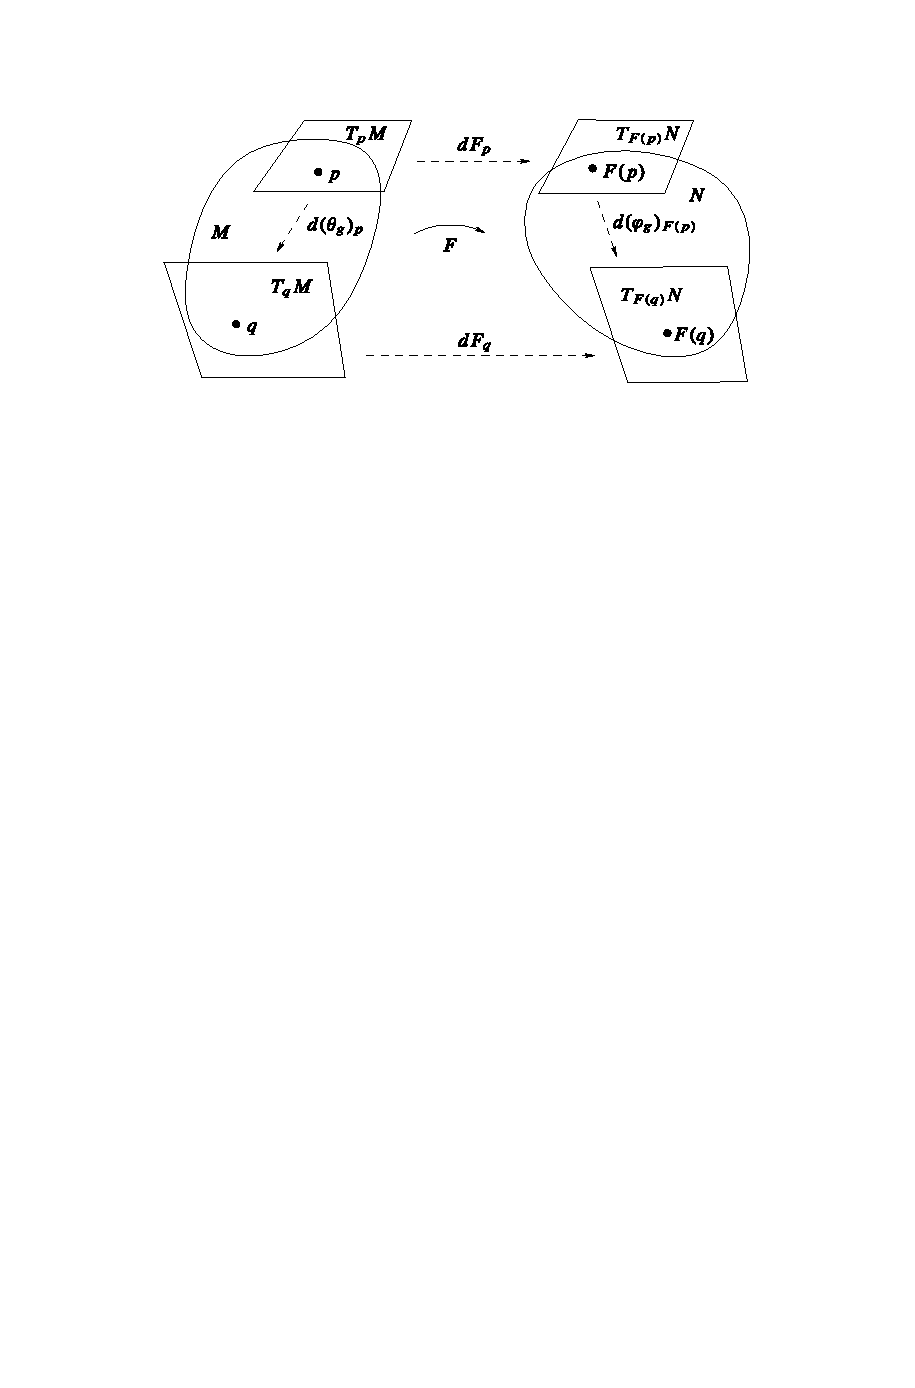
\includegraphics{pictures/equivariant-rank}
\caption{The equivariant rank theorem.}
\end{figure}
\begin{proof}
Let $\theta$ and $\varphi$ denote the $G$-actions on $M$ and $N$, respectively, and let $p$ and $q$ be arbitrary points in $M$. Choose $g\in G$ such that $\theta_g(p)=q$. (Such a $g$ exists because we are assuming that $G$ acts transitively on $M$.) Because $\varphi_g\circ F=\theta_g\circ F$, the following diagram commutes
\[\begin{tikzcd}
T_pM\ar[r,"dF_p"]\ar[d,swap,"d(\theta_g)_p"]&T_pN\ar[d,"d(\varphi_g)_{F(p)}"]\\
T_pM\ar[r,"dF_q"]&T_qN
\end{tikzcd}\]
Because the vertical linear maps in this diagram are isomorphisms, the horizontal ones have the same rank. In other words, the rank of $F$ is the same at any two arbitrary points $p,q\in M$, so $F$ has constant rank. The final statement follows from the global rank theorem.
\end{proof}
Here is an important application of the equivariant rank theorem. Suppose $G$ is a Lie group, $M$ is a smooth manifold, and $\theta:G\times M\to M$ is a smooth left action. For each $p\in M$, define a map $\theta^{(p)}:G\to M$ by
\[\theta^{(p)}(g)=g\cdot p\]
This is often called the orbit map, because its image is the orbit $G\cdot p$. In addition, the preimage $(\theta^{(p)})^{-1}(p)$ is the isotropy group $G_p$.
\begin{proposition}[\textbf{Properties of the Orbit Map}]\label{orbit map prop}
Suppose $\theta$ is a smooth left action of a Lie group $G$ on a smooth manifold $M$. For each $p\in M$, the orbit map $\theta^{(p)}:G\to M$ is smooth and has constant rank, so the isotropy group $G_p=(\theta^{(p)})^{-1}(p)$ is a properly embedded Lie subgroup of $G$. The induced map $F_p:G/G_p\to M$ on $G/G_p$ is an injective smooth immersion, so the orbit $G\cdot p$ is an immersed submanifold of $M$.
\end{proposition}
\begin{proof}
The orbit map is smooth because it is equal to the composition
\[G\approx G\times\{p\}\hookrightarrow G\times M\stackrel{\theta}{\to}M\]
It follows from the definition of a group action that $\theta^{(p)}$ is equivariant with respect to the action of $G$ on itself by left translation and the given action on $M$:
\[\theta^{(p)}(g'g)=(gg')\cdot p=g'\cdot(g\cdot p)=g'\cdot\theta^{(p)}(g)\]
Since $G$ acts transitively on itself, the equivariant rank theorem shows that $\theta^{(p)}$ has constant rank. Thus, $G_p$ is a properly embedded submanifold by Theorem~\ref{constant rank level set}, and a Lie subgroup by Proposition~\ref{Lie subgroup embedd mani}.\par
Now by quotient manifold theorem, the group $G/G_p$ has a unique smooth structure such that $\pi:G\to G_p$ is a smooth submersion. Therefore the induced map $F_p:G/G_p\to M$ defined by $F_p(gG_p)=\theta^{(p)}(g)$ is an injective smooth equivalent map with image $G\cdot p$. By the equivariant rank theorem, $F_p$ is then a smooth immersion, and thus the orbit (endowed with a suitable topology and smooth structure) is an immersed submanifold by Proposition~\ref{image immersion submani}.
\end{proof}
\begin{example}[\textbf{The Orthogonal Group}]\label{orthogonal group}
A real $n\times n$ matrix $A$ is said to be orthogonal if as a linear map $A:\R^n\to\R^n$ it preserves the Euclidean dot product:
\[(Ax)\cdot(Ay)=x\cdot y\for x,y\in\R^n\]
The set $\O(n)$ of all orthogonal $n\times n$ matrices is a subgroup of $\GL_n(\R)$, called the \textbf{orthogonal group} of degree $n$. It is easy to check that a matrix $A$ is orthogonal if and only if it takes the standard basis of $\R^n$ to an orthonormal basis, which is equivalent to the columns of $A$ being orthonormal. Since the $(i,j)$-entry of the matrix $A^TA$ is the dot product of the $i$-th and $j$-th columns of $A$, this condition is also equivalent to the requirement that $A^TA=I_n$.\par
Define a smooth map $\varPhi:\GL_n(\R)\to\mathcal{M}_n(\R)$ by $\varPhi(A)=A^TA$. Then $\O(n)$ is equal to the level set $\varPhi^{-1}(I_n)$. To show that $\varPhi$ has constant rank and therefore that $\O(n)$ is an embedded Lie subgroup, we show that $\varPhi$ is equivariant with respect to
suitable right actions of $\GL_n(\R)$. Let $\GL_n(\R)$ act on itself by right multiplication, and define a right action of $\GL_n(\R)$ on $\mathcal{M}_n(\R)$ by 
\[X\cdot B=B^TXB\for X\in\GL_n(\R), B\in\mathcal{M}_n(\R)\]
It is easy to check that this is a smooth action, and $\varPhi$ is equivariant because
\[\varPhi(AB)=(AB)^TAB=B^TA^TAB=B^T\varPhi(A)B=\varPhi(A)\cdot B\]
Thus, $\O(n)$ is a properly embedded Lie subgroup of $\GL_n(\R)$. It is compact because it is closed and bounded in $\mathcal{M}_n(\R)\approx\R^{n^2}$: closed because it is a level set of $\varPhi$, and bounded because every $A\in\O(n)$ has columns of norm $1$, and therefore satisfies $|A|=\sqrt{n}$.\par
To determine the dimension of $\O(n)$, we need to compute the rank of $\varPhi$. Because the rank is constant, it suffices to compute it at the identity $I_n\in\GL_n(\R)$. Thus for any $B\in T_{I_n}\GL_n(\R)=\mathcal{M}_n(\R)$, let $\gamma:(-\eps,\eps)\to\GL_n(\R)$ be the curve $\gamma(t)=I_n+tB$, and compute
\[d\varPhi_{I_n}B=\frac{d}{dt}\Big|_{t=0}\varPhi\circ\gamma(B)=\frac{d}{dt}\Big|_{t=0}(I_n+tB)^T(I_n+B)=B^T+B\]
From this formula, it is evident that the image of $d\varPhi_{I_n}$ is contained in the vector space of symmetric matrices. Conversely, if $B\in\mathcal{M}_n(\R)$ is an arbitrary symmetric $n\times n$ matrix, then $d\varPhi_{I_n}(1/2B)=B$. It follows that the image of $d\varPhi_{I_n}$ is exactly the space of symmetric matrices. This is a linear subspace of $\mathcal{M}_n(\R)$ of dimension $n(n+1)/2$, because each symmetric matrix is uniquely determined by its values on and above the main diagonal. It follows that $\O(n)$ is an embedded Lie subgroup of dimension 
\[n^2-\frac{n(n+1)}{2}=\frac{n(n-1)}{2}\]
\end{example}
\begin{example}[\textbf{The Special Orthogonal Group}]
The \textbf{special orthogonal group} of degree $n$ is defined as $\SO(n)=\O(n)\cap\SL_n(\R)$. Because every matrix $A\in\O(n)$ satisfies
\[1=\det I_n=\det(A^TA)=(\det A^T)(\det A)=(\det A)^2\]
it follows that $\det A=\pm1$ for all $A\in\O(n)$. Therefore, $\SO(n)$ is the open subgroup of $\O(n)$ consisting of matrices of positive determinant, and is therefore also an embedded Lie subgroup of dimension $n(n-1)/2$ in $\GL_n(\R)$. It is a compact group because it is a closed subset of $\O(n)$.
\end{example}
\begin{example}[\textbf{The Unitary Group}]
For any complex matrix $A$, the adjoint of $A$ is the matrix $A^*$ formed by conjugating the entries of $A$ and taking the transpose: $A=\widebar{A^T}$. For any positive integer $n$, the \textbf{unitary group} of degree $n$ is the subgroup $\U(n)\sub\GL_n(\C)$ consisting of complex $n\times n$ matrices whose columns form an orthonormal basis for $\C^n$ with respect to the Hermitian dot product $z\cdot w=\sum_iz^i\widebar{w^i}$. It is straightforward to check
that $\U(n)$ consists of those matrices $A$ such that $A^*A=I_n$.\par
Similar to Example~\ref{orthogonal group}, we define a map $\varPsi:\GL_n(\C)\to\mathcal{M}_n(\C)$ by $\varPsi(A)=A^*A$. Then $\U(n)=\varPsi^{-1}(I_n)$. We check that
\[\varPsi(AB)=B^*A^*AB=B^*\varPsi(A)B\]
so if we define an action of $\GL_n(\C)$ on $\mathcal{M}_n(\C)$ by
\[X\cdot B=B^*XB\for X\in\GL_n(\R),B\in\mathcal{M}_n(\C)\]
Then $\varPsi$ is an equivariant map, thus has constant rank. Now, to compute $d\varPsi_{I_n}$, we define a curve $\gamma:(-\eps,\eps)\to\GL_n(\C)$ by $\gamma(t)=I_n+tB$ where $B\in T_{I_n}\GL_n(\C)=\mathcal{M}_n(\C)$. We observe that
\[d\varPsi_{I_n}B=\frac{d}{dt}\Big|_{t=0}\varPsi\circ\gamma(B)=\frac{d}{dt}\Big|_{t=0}(I_n+tB)^*(I_n+B)=B^*+B\]
Hence the image of $d\varPsi_{I_n}$ is the \textbf{Hermitan matrix}, that is, matrix $B$ such that $B^*=B$. The dimension of the set of all Hermitan matrix is 
\[n+2\cdot\frac{n(n-1)}{2}=n^2\]
Thus $\U(n)$ is an properly embedded Lie subgroup of dimension $2n^2-n^2=n^2$.
\end{example}
\begin{example}[\textbf{The Special Unitary Group}]
The group $\SU(n)=\U(n)\cap\SL_n(\C)$ is called the complex special unitary group of degree $n$. For $A\in\U(n)$ we have
\[1=\det I_n=\det(A^*A)=(\det A^*)(\det A)=|\det A|^2\]
Thus there is an induced map $\det:\U(n)\to S^1$. Since $\dim S^1=1$ and $\SU(n)=\det^{-1}(1)$, it follows that $\SU(n)$ is a properly embedded $(n^2-1)$-dimensional Lie subgroup of $\U(n)$. Since the composition of smooth embeddings $\SU(n)\hookrightarrow\U(n)\hookrightarrow\GL_n(\C)$ is again a smooth embedding, this implies that $\SU(n)$ is also embedded in $\GL_n(\C)$.
\end{example}
\subsection{Semidirect products}
Suppose $N$ and $H$ are Lie groups, and $\theta:H\times N\to N$ is a smooth left action of $H$ on $N$. We define a new Lie group $N\rtimes_\theta H$, called a \textbf{semidirect product} of $H$ and $N$, as follows. As a smooth manifold, $N\rtimes_\theta H$ is just the Cartesian product $N\times H$ but the group multiplication is defined by
\[(n_1,h_1)(n_2,h_2)=(n_1\theta_{h_1}(n_2),h_1h_2)\]
\begin{example}[\textbf{The Euclidean Group}]\label{Euclidean group}
If we consider $\R^n$ as a Lie group under addition, then the natural action of $\O(n)$ on $\R^n$ is an action by automorphisms. The resulting semidirect product $\mathrm{E}(n)=\R^n\rtimes\O(n)$ is called the \textbf{Euclidean group}; its multiplication is given by $(b,A)(b',A')=(b+Ab',AA')$. It acts on $\R^n$ via
\[(b,A)\cdot x=b+Ax\]
It can be checked that
\[\big((b,A)(b',A')\big)\cdot x=(b+Ab',AA')x=b+Ab'+AA'x=(b,A)\cdot (b'+A'x)=(b,A)\cdot((b',A')\cdot x)\]
so this action is well defined. This action preserves lines, distances, and angle measures, and thus all of the relationships of Euclidean geometry.\par 
A faithful representation of $\mathrm{E}(n)$ is given by the map $\rho:\mathrm{E}(n)\to\GL_{n+1}(\R)$ defined in block form by
\[\rho(b,A)=\begin{pmatrix}
A&b\\
0&1
\end{pmatrix}\]
\end{example}
The following result gives a extremely useful method to characterize semidirect products. We will use it to give some examples of Lie groups.
\begin{proposition}\label{semidirect product iff}
Suppose $G,N$, and $H$ are Lie groups. Prove that $G$ is isomorphic to a semidirect product $N\rtimes H$ if and only if there are Lie group homomorphisms $\varphi:G\to H$ and $\psi:H\to G$ such that $\varphi\circ\psi=\mathrm{id}_H$ and $\ker\varphi\cong N$.
\end{proposition}
\begin{proof}
If $G\approx N\rtimes H$, then the projection on $H$ and the embedding ot $H$ in $G$ satisfy the conditions.\par
Conversely, assume the existence of $\varphi$ and $\psi$:
\[\begin{tikzcd}
1\ar[r]&N\ar[r,hook]&G\ar[r,"\varphi"]&H\ar[l,bend left=30,"\psi"]\ar[r]&1
\end{tikzcd}\]
Since this sequence is split exact, we can regard $N,H$ as subgroups of $G$ such that $N\cap H=\{e\}$ and $NH=G$. Since $N$ is normal in $G$, $H$ act on $N$ by conjugation, so the map $(n,h)\mapsto nh$ is an isomorphsim from $G$ to $N\rtimes H$.
\end{proof}
\begin{proposition}\label{Lie groups as semidirect product}
The following Lie groups are isomorphic to semidirect products as shown.
\begin{itemize}
\item[(a)] $\O(n)\cong\SO(n)\rtimes\O(1)$.
\item[(b)] $\U(n)\cong\SU(n)\rtimes\U(1)$.
\item[(c)] $\GL_n(\R)\cong\SL_n(\R)\rtimes\R^*$.
\item[(d)] $\GL_n(\C)\cong\SL_n(\C)\rtimes\C^*$.
\end{itemize}
\end{proposition}
\begin{proof}
In order to apply Proposition~\ref{semidirect product iff}, we consider the maps
\[\det:\GL_n(\R)\to\R^*,\quad \psi:\R^*\to\GL_n(\R),\quad x\mapsto xI_n\]
and
\[\det:\O(n)\to\{\pm 1\},\quad \psi:\{\pm 1\}\to\O(n),\quad x\mapsto xI_n.\]
we have $\ker\det=\det^{-1}(1)=\SL_n(\R)$, or $\ker\det=\SO(n)$. The claim therefore follows.
\end{proof}
There is a close connection between representations and group actions. Let $G$ be a Lie group and $V$ be a finite-dimensional vector space. An action of $G$ on $V$ is said to be a linear action if for each $g\in G$, the map from $V$ to itself given by $x\mapsto g\cdot x$ is linear. For example, if $\rho:G\to\GL(V)$ is a representation of $G$, there is an associated smooth linear action of $G$ on $V$ given by $g\cdot x:=\rho(g)x$. The next proposition shows that every linear action is of this type.
\begin{proposition}
Let $G$ be a Lie group and $V$ be a finite-dimensional vector space. A smooth left action of $G$ on $V$ is linear if and only if it is of the form $g\cdot x=\rho(g)x$ for some representation $\rho$ of $G$.
\end{proposition}
\begin{proof}
Every action induced by a representation is evidently linear. To prove the converse, assume that we are given a linear action of $G$ on $V$. The hypothesis implies that for each $g\in G$ there is a linear map $\rho(g)\in\GL(V)$ such that $g\cdot x=\rho(g)x$ for all $x\in V$. The group action condition implies $\rho(g_1g_2)=\rho(g_1)\rho(g_2)$, so $\rho:G\to\GL(V)$ is a group homomorphism. Thus, to show that it is a Lie group representation, we need only show that it is smooth. Choose a basis $\{E_i\}$ for $V$, and for each $i$ let $\pi^i:V\to\R$ be the projection onto the $i$ th coordinate with respect to this basis. If we let $(\rho_j^i(g))$ denote the matrix entries of $\rho(g)$ with respect to this basis, it follows that $\rho_j^i(g)=\pi^i(g\cdot E_j)$, so each function $\rho_j^i$ is a composition of smooth functions. Because the matrix entries form global smooth coordinates for $\GL(V)$, this implies that $\rho$ is smooth.
\end{proof}
\subsection{Exercise}
\begin{exercise}\label{Lie group operator diff}
Let $G$ be a Lie group.
\begin{itemize}
\item[(a)] Let $m$ be the multiplication, show that the differential $dm_{(e,e)}:T_eG\oplus T_eG\to T_eG$ is given by
\[dm_{(e,e)}(X,Y)=X+Y\for X,Y\in T_eG\]
\item[(b)] Let $i$ be the inverse map, show that the differential $di_{e}:T_eG\to T_eG$ is given by
\[di_e(X)=-X\for X\in T_eG\]
\end{itemize}
\end{exercise}
\begin{proof}
For part (a), fix $g,h\in G$. Then since $T_{(g,h)}(G\times G)\cong T_gG\oplus T_hG$, we have
\[dm_{(g,h)}(X,Y)=d(m\circ j^h)_g(X)+d(m\circ \iota_g)_hY\]
for $X\in T_gG,Y\in T_hG$, where $j^h(x)=(x,h)$ and $\iota_g(x)=(g,x)$. Thus we have
\[dm_{(g,h)}(X,Y)=d(R_h)_gX+d(L_g)_hY\]

For part (b), let $X\in T_eG$ and define a map
\[\alpha:G\to G\times G,\quad g\mapsto(g,i(g))\]
Then we have
\[d\alpha_e(X)=(X,di_eX)\]
Since $m\circ\alpha=e$, we conclude by the chain rule
\[dm_{e,e}\circ d\alpha_e(X)=dm_{(e,e)}(X,di_e(X))=X+di_e(X)=0\]
This implies $di_e(X)=-X$.\par
Now note that for any $g\in G$ we have $i=R_{g^{-1}}\circ i\circ L_{g^{-1}}$ since
\[R_{g^{-1}}\circ i\circ L_{g^{-1}}(x)=R_{g^{-1}}\circ i(g^{-1}x)=x^{-1}gg^{-1}=x^{-1}\]
So using this and the chain rule we have
\[di_g(X)=d(R_{g^{-1}})_e\circ di_e\circ d(L_{g^{-1}})_g(X)=-d(R_{g^{-1}})_e\circ d(L_{g^{-1}})_g(X)\for X\in T_gG\]
which is the desired claim.
\end{proof}
\begin{exercise}\label{det diff}
Let $\det:\GL_n(\R)\to\R$ denote the determinant function. For any $A\in\mathcal{M}_n(\R)$, show that
\[\frac{d}{dt}\Big|_{t=0}\det(I_n+tA)=\tr A.\]
From this, conclude that, for $X\in\GL_n(\R)$ and $B\in T_X\GL_n(\R)\approx\mathcal{M}_n(\R)$,
\[d(\det)_X(B)=(\det X)\tr(X^{-1}B).\]
\end{exercise}
\begin{proof}
Let $B(t)=(b_{ij}(t)):I\to\mathcal{M}_n(\R)$ be a smooth curve such that $B(0)=I_n$. Then expanding the determinant along the first column, we have
\[\det(B(t))=\sum_{i=1}^{n}(-1)^{i+1}b_{1i}(t)\cdot\det(B_{1i}(t)),\]
where $B_{ij}$ is the minor of $B$ at position $(i,j)$. Now differentiate both sides, we get
\[\frac{d}{dt}\Big|_{t=0}\det(B(t))=\sum_{i=1}^{n}(-1)^{i+1}\Big[b'_{1i}(0)\cdot\det(B_{1i}(0))+b_{1i}(0)\cdot\frac{d}{dt}\Big|_{t=0}\det(B_{11}(t))\Big].\]
By $B(0)=I_n$, the RHS is simplified into
\[\frac{d}{dt}\Big|_{t=0}\det(B(t))=b'_{11}(0)+\frac{d}{dt}\Big|_{t=0}\det(B_{1i}(t)).\]
Now by a simple induction we get
\[\frac{d}{dt}\Big|_{t=0}\det(B(t))=b'_{11}(0)+\cdots+b'_{nn}(0)=\tr(B'(0)).\]
Now we define the curve $\gamma(t)=X+tB$ for $B\in T_X\GL_n(\R)$, and observe that
\[\det(X+tB)=\det(X)\det(I_n+tX^{-1}B)\]
Thus by Corollary~\ref{compute diff by curve},
\[d(\det)_X(B)=\frac{d}{dt}\Big|_{t=0}(\det\circ\gamma)=\det(X)\frac{d}{dt}\Big|_{t=0}\det(I_n+tX^{-1}B)=\det(X)\tr(X^{-1}B)\]
which is the desired result.
\end{proof}
\begin{exercise}
Suppose a connected topological group $G$ acts continuously on a discrete space $K$. Show that the action is trivial. 
\end{exercise}
\begin{proof}
Let $\rho:G\times K\to K$ be the action. Note that the connected component of $G\times K$ is $G\times\{x\}$ for $x\in K$. For any $x_0\in K$, the set $U:=\rho^{-1}(x_0)$ is closed and open in $G\times K$, thus is of the form $G\times\{y\}$. Since $(e,x_0)\sub U$, we conclude $U=G\times\{x_0\}$. Thus $\rho$ is trivial on $x_0$. Since $x_0$ is arbitrary, this implies $\rho$ is trivial on $K$.
\end{proof}
\begin{exercise}
Considering $S^{2n+1}$ as the unit sphere in $\C^{n+1}$, define an action of $S^1$ on $S^{2n+1}$, called the \textbf{Hopf action}, by
\[z(w^1,\dots,w^{n+1})=(zw^1,\dots,zw^{n+1})\]
Show that this action is smooth and its orbits are disjoint unit circles in $\C^{n+1}$ whose union is $S^{2n+1}$.
\end{exercise}
\begin{proof}
Note that this action is free on $S^1$, so by Proposition~\ref{orbit map prop} each orbit is an immersed submanifold. Since $S^1$ is a compact set, it is in fact an embedded submanifold. So each orbit is a unite circle in $\C^{n+1}$.
\end{proof}
\begin{exercise}
Show that $\SO(2)$, $U(1)$, and $S^1$ are all isomorphic as Lie groups.
\end{exercise}
\begin{proof}
The subgroup $\SO(2)$ takes the following from 
\[\begin{pmatrix}
\cos\varphi&-\sin\varphi\\
\sin\varphi&\cos\varphi
\end{pmatrix}\]
Thus $\SO(2)\approx S^1$. The subgroup $\U(1)$ consists of $1\times 1$ matrix of modulus $1$, which may be regarded as $S^1$.
\end{proof}
\begin{exercise}
Prove that $\SU(2)$ is diffeomorphic to $S^3$.
\end{exercise}
\begin{proof}
Let $U\in\GL_n(\C)$,
\[U=\begin{pmatrix}
z_1&z_2\\
z_3&z_4
\end{pmatrix}\]
From the conditions $\det U=1$ and $U^*U=I_n$, we get
\[
\left\{\begin{array}{l}
z_1z_4-z_2z_3=1\\
|z_1|^2+|z_2|^2=1\\
|z_3|^2+|z_4|^2=1\\
z_1\widebar{z}_3+z_2\widebar{z}_4=0
\end{array}\right. \]
Let's assume $z_1=z\widebar{z}_4$ where $z\in\C$, then $z_2=-z\widebar{z}_3$. Plugging this into the equations we get 
\[|z|^2(|z_3|^2+|z_4|^2)=1,\quad z(|z_3|^2+|z_4|^2)=1\]
Thus $z=1$, and $U$ has the following form
\[\begin{pmatrix}
z_1&-\widebar{z}_2\\
z_2&\widebar{z}_1
\end{pmatrix}\]
where $|z_1|^2+|z_2|^2=1$. Since $S^3$ can be viewed as the set $\{|z_1|^2+|z_2|^2=1\}$ in $\C^2$, this implies $\SU(2)\approx S^3$.
\end{proof}
\begin{exercise}
Let $\H=\C\times\C$ be the quaternions. The multiplication of $\H$ is given by
\[\mathbf{i}^2=\mathbf{j}^2=\mathbf{k}^2=\mathbf{i}\mathbf{j}\mathbf{k}=-\mathbf{1}\] 
By considering $\H$ as a two dimensional complex vector space, find a representation of $\H$ into $\GL_2(\C)$.
\end{exercise}
\begin{proof}
Thus a representation $\rho:\H\to\GL_2(\C)$ given by \[\rho(z,w)=\begin{pmatrix}
z&w\\
-\widebar{w}&\widebar{z}
\end{pmatrix}.\]
Since the multiplication in $\H$ can be written as
\[(a,b)(c,d)=(ac-\widebar{d}b,da+b\widebar{c})\]
when the base ring is commutative, this can be realized into marix multiplications.\par
Note that
\[\rho(\mathbf{1})=\begin{pmatrix}
1&0\\
0&1
\end{pmatrix},\quad\rho(\mathbf{i})=\begin{pmatrix}
i&0\\
0&-i
\end{pmatrix},\quad\rho(\mathbf{j})=\begin{pmatrix}
0&1\\
-1&0
\end{pmatrix},\quad\rho(\mathbf{k})=\begin{pmatrix}
0&i\\
i&0
\end{pmatrix},\quad\]
Due to this, $\H$ has another definition: consider $\mathcal{M}_2(\C)$, the set 
\[\H\cong\{M\in\mathcal{M}_2(\C):M^*M=aI_2,a\in\R,\det(M)\geq 0\}\]
Note that $\C$ can also be defined in the same way:
\[\C\cong\{M\in\mathcal{M}_2(\R):M^*M=aI_2,a\in\R,\det(M)\geq 0\}\]
\end{proof}
\section{Lie algebras}
\subsection{The Lie algebra of a Lie group}
One of the most important applications of Lie brackets occurs in the context of Lie groups. Suppose $G$ is a Lie group. Recall that $G$ acts smoothly and transitively on itself by left translation: $L_g(h)=gh$. A vector field $X$ on $G$ is said to be \textbf{left-invariant} if it is invariant under all left translations, in the sense that it is $L_g$-related to itself for every $g\in G$. More explicitly, this means
\[d(L_g)_{g'}(X_{g'})=X_{gg'}\quad\text{for all }g,g'\in G.\]
Since $L_g$ is a diffeomorphism, this can be abbreviated by writing $(L_g)_*X=X$ for every $g\in G$.\par
Because $(L_g)_*(aX+bY)=a(L_g)_*X+b(L_g)_*Y$, the set of all smooth left-invariant vector fields on $G$ is a linear subspace of $\X(G)$. But it is much more than that. The central fact is that it is closed under Lie brackets.
\begin{proposition}
Let $G$ be a Lie group, and suppose $X$ and $Y$ are smooth left-invariant vector fields on $G$. Then $[X,Y]$ is also left-invariant.
\end{proposition}
\begin{proof}
Let $g\in G$ be arbitrary. Since $(L_g)_*X=X$ and $(L_g)_*Y=Y$ by definition of left-invariance, it follows from Corollary~\ref{Lie bracket pushforward} that
\[(L_g)_*[X,Y]=[(L_g)_*X,(L_g)_*Y]=[X,Y]\]
Thus, $[X,Y]$ is $L_g$-related to itself for each $g$, which is to say it is left-invariant.
\end{proof}
A \textbf{Lie algebra} (over $\R$) is a real vector space $\g$ endowed with a map called the bracket from $\g\times\g$ to $\g$, usually denoted by $(X,Y)\mapsto[X,Y]$, that satisfies the following properties for all $X,Y,Z\in\g$:
\begin{itemize}
\item Bilinearity: For $a,b\in\R$,
\[[aX+bY,Z]=a[X,Z]+b[Y,Z],\quad [X,aY+bZ]=a[X,Y]+b[X,Z].\]
\item Antisymmetry:
\[[X,Y]=-[Y,X]\]
\item Jacobi identity:
\[[X,[Y,Z]]+[Y,[Z,X]]+[Z,[X,Y]]=0\]
\end{itemize}
Notice that the Jacobi identity is a substitute for associativity, which does not hold in general. If $\g$ is a Lie algebra, a linear subspace $\h\sub\g$ is called a Lie subalgebra of $\g$ if it is closed under brackets. In this case $\h$ is itself a Lie algebra with the restriction of the same bracket.\par
If $\g$ and $\h$ are Lie algebras, a linear map $A:\g\to\h$ is called a \textbf{Lie algebra homomorphism} if it preserves brackets: $A[X,Y]=[AX,AY]$. An invertible Lie algebra homomorphism is called a \textbf{Lie algebra isomorphism}. If there exists a Lie algebra isomorphism from $\g$ to $\h$, we say that they are \textbf{isomorphic as Lie algebras}.
\begin{example}[\textbf{Lie Algebras}]
\mbox{}
\begin{itemize}
\item[(a)] The space $\X(M)$ of all smooth vector fields on a smooth manifold $M$ is a Lie algebra under the Lie bracket by Proposition~\ref{Lie bracket prop}.
\item[(b)] If $G$ is a Lie group, the set of all smooth left-invariant vector fields on $G$ is a Lie subalgebra of $\X(G)$ and is therefore a Lie algebra.
\item[(c)] The vector space $\mathcal{M}_n(\R)$ $n\times n$ real matrices becomes an $n^2$-dimensional Lie algebra under the \textbf{commutator bracket}:
\[[A,B]=AB-BA\]
Bilinearity and antisymmetry are obvious from the definition, and the Jacobi identity follows from a straightforward calculation. When we are regarding $\mathcal{M}_n(\R)$ as a Lie algebra with this bracket, we denote it by $\gl(n,\R)$.
\item[(d)] Similarly, $\gl(n,\C)$ is the $2n^2$-dimensional $($real$)$ Lie algebra obtained by endowing $\mathcal{M}_n(\C)$ with the commutator bracket.
\item[(e)] If $V$ is a vector space, the vector space of all linear maps from $V$ to itself becomes a Lie algebra, which we denote by $\gl(V)$, with the commutator bracket:
\[[A,B]=A\circ B-B\circ A\]
Under our usual identification of $n\times n$ matrices with linear maps from $\R^n$ to itself, $\gl(\R^n)$ is the same as $\gl(n,\R)$.
\item[(f)]Any vector space $V$ becomes a Lie algebra if we define all brackets to be zero. Such a Lie algebra is said to be \textbf{abelian}. (The name reflects the fact that brackets in most Lie algebras, as in the preceding examples, are defined as commutators in terms of underlying associative products, so all brackets are zero precisely when the underlying product is commutative; it also reflects the connection between abelian Lie algebras and abelian Lie groups.)
\end{itemize}
\end{example}
Example (b) is the most important one. The Lie algebra of all smooth left-invariant vector fields on a Lie group $G$ is called the Lie algebra of $G$, and is denoted by $\Lie(G)$. The fundamental fact is that $\Lie(G)$ is finite-dimensional, and in fact has the same dimension as $G$ itself, as the following theorem shows.
\begin{theorem}\label{Lie algrbra iso tangent space}
Let $G$ be a Lie group. The evaluation map $\eps:\Lie(G)\to T_eG$, given by $\eps(X)=X_e$, is a vector space isomorphism. Thus, $\Lie(G)$ is finite-dimensional, with dimension equal to $\dim G$.
\end{theorem}
\begin{proof}
It is clear from the definition that $\eps$ is linear over $\R$. It is easy to prove that it is injective: if $\eps(X)=X_e=0$ for some $X\in\Lie(G)$, then left-invariance of $X$ implies that $X_g=d(L_g)_eX_e=0$ for every $g\in G$, so $X=0$.\par
To show that $\eps$ is surjective, let $v\in T_eG$ be arbitrary, and define a (rough) vector field $v^L$ on $G$ by
\begin{align}\label{Lie algebra iso-1}
v^L_g=d(L_g)_e(v)
\end{align}
If there is a left-invariant vector field on $G$ whose value at the identity is $v$, clearly it has to be given by this formula.\par
First we need to check that $v^L$ is smooth. By Proposition~\ref{vector field smooth by function}, it suffices to show that $v^Lf$ is smooth whenever $f\in C^\infty(G)$. Choose a smooth curve $\gamma:(-\delta,\delta)\to G$ such that $\gamma(0)=e$ and $\gamma'(0)=v$. Then for all $g\in G$,
\begin{align*}
(v^Lf)(g)=v^L_gf=d(L_g)_e(v)(f)=\gamma'(0)(f\circ L_g)=\frac{d}{dt}\Big|_{t=0}(f\circ L_g\circ\gamma)(t)
\end{align*}
If we define $\varphi:(-\delta,\delta)\times G\to G$ by $\varphi(t,g)=f\circ L_g\circ\gamma(t)=f(g\gamma(t))$, the computation above shows that $(v^Lf)(g)=\partial\varphi/\partial t(0,g)$. Because $\varphi$ is a composition of group multiplication, $f$ and $\gamma$, it is smooth. It follows that $\partial\varphi/\partial t(0,g)$ depends smoothly on $g$, so $v^Lf$ is smooth.\par
Next we show that $v^L$ is left-invariant, which is to say that $d(L_h)_g(v^L|_g)=v^L|_{hg}$ for all $g,h\in G$. This follows from the definition of $v^L$ and the fact that $L_h\circ L_g=L_{hg}$:
\[d(L_h)_g(v^L|_g)=d(L_h)_g\circ d(L_g)_e(v)=d(L_{hg})_e(v)=v^L|_{hg}\]
Thus $v^L\in\Lie(G)$. Since $L_e$ (left translation by the identity) is the identity map of $G$, it follows that $\eps(v^L)=v$, so $\eps$ is surjective.
\end{proof}
Given any vector $v\in T_eG$, we continue to use the notation $v^L$ to denote the smooth left-invariant vector field defined by $(\ref{Lie algebra iso-1})$.\par
It is worth observing that the preceding proof also shows that the assumption of smoothness in the definition of $\Lie(G)$ is unnecessary.
\begin{corollary}\label{Lie rough left-inv}
Every left-invariant rough vector field on a Lie group is smooth.
\end{corollary}
\begin{proof}
Let $X$ be a left-invariant rough vector field on a Lie group $G$, and let $v=X_e$. The fact that $X$ is left-invariant implies that $X=v^L$, which is smooth.
\end{proof}
The existence of global left-invariant vector fields also yields the following important property of Lie groups. Recall that a smooth manifold is said to be \textit{parallelizable} if it admits a smooth global frame. If $G$ is a Lie group, a local or global frame consisting of left-invariant vector fields is called a \textbf{left-invariant frame}.
\begin{corollary}\label{Lie group parallelizable}
Every Lie group admits a left-invariant smooth global frame, and therefore every Lie group is parallelizable.
\end{corollary}
\begin{proof}
If $G$ is a Lie group, every basis for $\Lie(G)$ is a left-invariant smooth global frame for $G$.
\end{proof}
\begin{example}
Let us determine the Lie algebras of some familiar Lie groups.
\begin{itemize}
\item[(a)] Euclidean space $\R^n$: If we consider $\R^n$ as a Lie group under addition, left translation by an element $b\in\R^n$ is given by the affine map $L_b(x)=b+x$, whose differential $dL_b$ is represented by the identity matrix in standard coordinates. Thus a vector field $X_i\partial/\partial x^i$ is left-invariant if and only if its coefficients $X_i$ are constants. Because the Lie bracket of two constant-coefficient vector fields is zero, the Lie algebra of $\R^n$ is abelian, and is isomorphic to $\R^n$ itself with the trivial bracket. In brief, $\Lie(\R^n)\cong\R^n$.
\item[(b)] The circle group $S^1$: In terms of appropriate angle coordinates, each left translation has a local coordinate representation of the form $\theta\mapsto\theta+c$. Since the differential of this map is the identity matrix, it follows that the vector field $d/d\theta$ is left-invariant, and is therefore a basis for the Lie algebra of $S^1$. This Lie algebra is $1$-dimensional and abelian, and therefore $\Lie(S^1)\cong\R$. Similarly, $\Lie(T^n)\cong\R^n$.
\end{itemize}
\end{example}
The Lie groups $\R^n$, $S^1$, and $T^n$ are abelian, and as the discussion above shows, their Lie algebras turn out also to be abelian. This is no accident: every abelian Lie group has an abelian Lie algebra. Later, we will see that the converse is true provided that the group is connected.\par
We conclude this section by analyzing the Lie algebra of the most important nonabelian Lie group of all, the general linear group. Theorem~\ref{Lie algrbra iso tangent space} gives a vector space isomorphism between $\Lie(\GL_n(\R))$ and the tangent space to $\GL_n(\R)$ at the identity matrix $I_n$. Because $\GL_n(\R)$ is an open subset of the vector space $\gl_n(\R)$, its tangent space is naturally isomorphic to $\gl_n(\R)$ itself. The composition of these two isomorphisms gives a vector space isomorphism $\Lie(\GL_n(\R))\cong\gl(n,\R)$.\par
The vector spaces $\Lie(\GL_n(\R))$ and $\gl(n,\R)$ have independently defined Lie algebra structures---the first coming from Lie brackets of vector fields, and the second from commutator brackets of matrices. The next proposition shows that the natural vector space isomorphism between these spaces is in fact a Lie algebra isomorphism.
\begin{proposition}[\textbf{Lie Algebra of the General Linear Group}]
The composition of the natural maps
\begin{equation}
\Lie(\GL_n(\R))\to T_{I_n}\GL_n(\R)\to\gl(n,\R)
\end{equation}
gives a Lie algebra isomorphism between $\Lie(\GL_n(\R))$ and the matrix algebra $\gl(n,\R)$.
\end{proposition}
\begin{proof}
Using the matrix entries $(X^i_j)$ as global coordinates on $\GL_n(\R)\sub\gl_n(\R)$, the natural isomorphism $T_{I_n}\GL_n(\R)\cong\gl(n,\R)$ takes the form
\[A^i_j\frac{\partial}{\partial X^i_j}\Big|_{I_n}\Longleftrightarrow A^i_j\]
Let $\g$ denote the Lie algebra of $\GL_n(\R)$. Any matrix $A=(A^i_j)\in\gl(n,\R)$ determines a left-invariant vector field $A^L\in\g$ defined by $(\ref{Lie algebra iso-1})$, which in this case becomes
\[A^L|_Y=d(L_Y)_{I_n}(A)=d(L_Y)_{I_n}\Big(A^i_j\frac{\partial}{\partial X^i_j}\Big|_{I_n}\Big)\]
Since $L_Y$ is the restriction to $\GL_n(\R)$ of the linear map $A\mapsto YA$ on $\gl(n,\R)$, its differential is represented in coordinates by exactly the same linear map. In other words, the left-invariant vector field $A^L$ determined by $A$ is the one whose value at $Y\in\GL_n(\R)$ is
\begin{equation}\label{Lie algrbra gl(n,R)}
A^L|_Y=Y^i_jA^j_k\frac{\partial}{\partial X^i_k}\Big|_Y
\end{equation}
Thus by useing the coordinates function $(X^i_j)$, we can write $A^L$ as
\[A^L=X^i_jA^j_k\frac{\partial}{\partial X^i_k}\]

Given two matrices $A,B\in\gl(n,\R)$, the Lie bracket of the corresponding left-invariant vector fields is given by
\begin{align*}
[A^L,B^L]&=\Big[X^i_jA^j_k\frac{\partial}{\partial X^i_k},X^p_qB^q_r\frac{\partial}{\partial X^p_r}\Big]\\
&=X^i_jA^j_k\frac{\partial(X^p_qB^q_r)}{\partial X^i_k}\frac{\partial}{\partial X^p_r}-X^p_qB^q_r\frac{\partial(X^i_jA^j_k)}{\partial X^p_r}\frac{\partial}{\partial X^i_k}\\
&=X^i_jA^j_kB^k_r\frac{\partial}{\partial X^i_r}-X^p_qB^q_rA^r_k\frac{\partial }{\partial X^p_k}\\
&=X^i_jA^j_kB^k_r\frac{\partial}{\partial X^i_r}-X^i_jB^j_kA^k_r\frac{\partial}{\partial X^i_k}\\
&=X^i_j(A^j_kB^k_r-B^j_kA^k_r)\frac{\partial}{\partial X^i_k}
\end{align*}
where we have used the fact that $\partial X^p_q/\partial X^i_k$ is equal to $1$ if $p=i$ and $q=k$, and $0$ otherwise, and $A^i_j$ and $B^i_j$ are constants. Evaluating this last expression when $X$ is equal to the identity matrix, we get
\[[A^L,B^L]_{I_n}=(A^i_kB^k_r-B^i_kA^k_r)\frac{\partial}{\partial X^i_k}\Big|_{I_n}\]
This is the vector corresponding to the matrix commutator bracket $[A,B]$. Since the left-invariant vector field $[A^L,B^L]$ is determined by its value at the identity, this implies that
\[[A^L,B^L]=[A,B]^L\]
which is precisely the statement that the composite map is a Lie algebra isomorphism.
\end{proof}
There is an analogue of this result for abstract vector spaces. If $V$ is any finitedimensional real vector space, recall that we have defined $\GL(V)$ as the Lie group of invertible linear transformations of $V$, and $\gl(V)$ as the Lie algebra of all linear transformations. Just as in the case of $\GL_n(\R)$, we can regard $\GL(V)$ as an open submanifold of $\gl(V)$, and thus there are canonical vector space isomorphisms
\begin{align}\label{Lie algebra GL(V) iso-1}
\Lie(\GL(V))\to T_{\mathrm{id}}\GL(V)\to\gl(V)
\end{align}
\begin{corollary}\label{Lie algebra GL(V) iso}
If $V$ is any finite-dimensional real vector space, the composition of the canonical isomorphisms in $(\ref{Lie algebra GL(V) iso-1})$ yields a Lie algebra isomorphism between $\Lie(\GL(V))$ and $\gl(V)$.
\end{corollary}

\subsection{Induced Lie algebra homomorphisms}
The importance of the Lie algebra of a Lie group stems, in large part, from the fact that each Lie group homomorphism induces a Lie algebra homomorphism, as the next theorem shows.
\begin{theorem}[\textbf{Induced Lie Algebra Homomorphisms}]\label{Lie algebra induce}
Let $G$ and $H$ be Lie groups, and let $\g$ and $\h$ be their Lie algebras. Suppose $F:G\to H$ is a Lie group homomorphism. For every $X\in g$, there is a unique vector field in $\h$ that is $F$-related to $X$. With this vector field denoted by $F_*X$, the map $F_*:\g\to\h$ so defined is a Lie algebra homomorphism.
\end{theorem}
\begin{figure}[htbp]
\centering
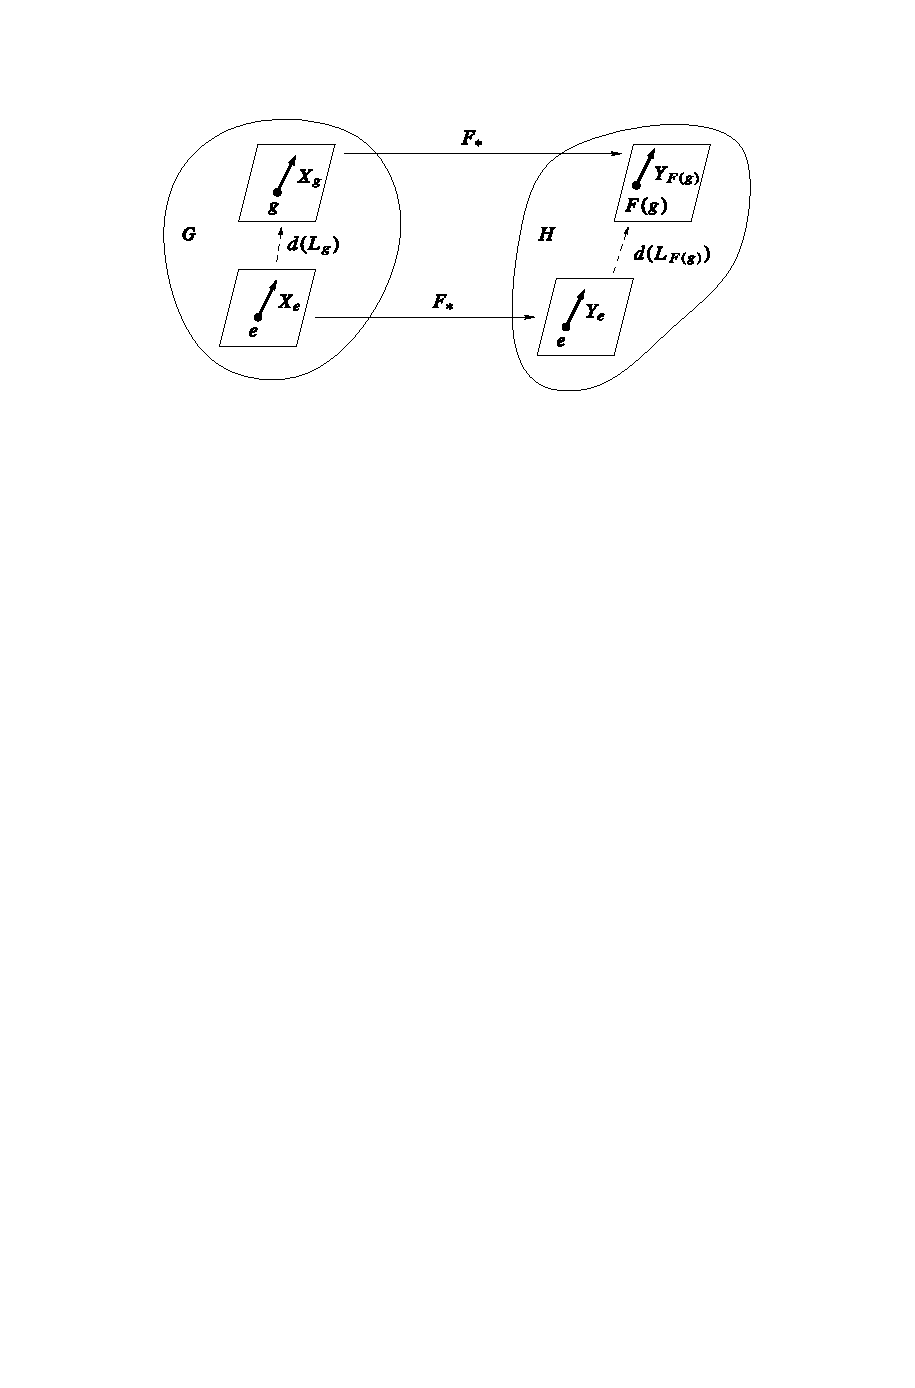
\includegraphics{pictures/induced-Lie-homo}
\caption{The induced Lie algebra homomorphism.}
\end{figure}
\begin{proof}
If there is any vector field $Y\in\h$ that is $F$-related to $X$, it must satisfy $Y_e=dF_e(X_e)$, and thus it must be uniquely determined by
\[Y=(Y_e)^L=(dF_e(X_e))^L\]
To show that this $Y$ is $F$-related to $X$, we note that the fact that $F$ is a homomorphism implies
\begin{align*}
F(gg')=F(g)F(g')&\Rightarrow F(L_gg')=L_{F(g)}F(g')\\
&\Rightarrow F\circ L_g=L_{F(g)}\circ F\\
&\Rightarrow dF\circ d(L_g)=d(L_{F(g)})\circ dF
\end{align*}
Thus,
\[dF(X_g)=dF\circ d(L_g)(X_e)=d(L_{F(g)})\circ dF(X_e)=d(L_{F(g)})(Y_e)=Y_{F(g)}\]
This says precisely that $X$ and $Y$ are $F$-related.\par
For each $X\in g$, let $F_*X$ denote the unique vector field in $\h$ that is $F$-related to $X$. It then follows immediately from the naturality of Lie brackets that $F_*[X,Y]=[F_*X,F_*Y]$, so $F_*$ is a Lie algebra homomorphism.
\end{proof}
The map $F_*:\g\to\h$ whose existence is asserted in this theorem is called the \textbf{induced Lie algebra homomorphism}. Note that the theorem implies that for any left-invariant vector field $X\in g$, $F_*X$ is a well-defined smooth vector field on $H$, \textit{even though $F$ may not be a diffeomorphism}.
\begin{proposition}[\textbf{Properties of Induced Homomorphisms}]
\mbox{}
\begin{itemize}
\item[(a)] The homomorphism $(\mathrm{id})_*:\Lie(G)\to\Lie(G)$ induced by the identity map of $G$ is the identity of $\Lie(G)$.
\item[(b)] If $F_1:G\to H$ and $F_2:H\to K$ are Lie group homomorphisms, then
\[(F_2\circ F_1)_*=(F_2)_*\circ(F_1)_*\]
\item[(c)] Isomorphic Lie groups have isomorphic Lie algebras.
\end{itemize}
\end{proposition}
\begin{proof}
These all follow from the property of the differential $F_*$.
\end{proof}
Therefore, we obtain a functor from the category of Lie groups to the category of Lie algebras. 
\subsection{Lie subalgebras and Lie subgroups}
If $G$ is a Lie group and $H\sub G$ is a Lie subgroup, we might hope that the Lie algebra of $H$ would be a Lie subalgebra of that of $G$. However, elements of $\Lie(H)$ are vector fields on $H$, not $G$, and so, strictly speaking, are not elements of $\Lie(G)$. Nonetheless, the next proposition gives us a way to view $\Lie(H)$ as a subalgebra of $\Lie(G)$.
\begin{proposition}\label{Lie subalgebra}
Suppose $H\sub G$ is a Lie subgroup, and $\iota:H\hookrightarrow G$ is the inclusion map. There is a Lie subalgebra $\h\in\Lie(G)$ that is canonically isomorphic to $\Lie(H)$, characterized by either of the following descriptions:
\[\h=\iota_*(\Lie(H))=\{X\in\Lie(G):X_e\in T_eH\}\]
\end{proposition}
\begin{proof}
Because the inclusion map $\iota:H\hookrightarrow G$ is a Lie group homomorphism, $\iota_*(\Lie(H))$ is a Lie subalgebra of $\Lie(G)$. 
By the way we defined the induced Lie algebra homomorphism, this subalgebra is precisely the set of left-invariant vector fields on $G$ whose values at 
the identity are of the form $d\iota_e(v)$ for some $v\in T_eH$. Since the differential $d\iota_e:T_eH\to T_eG$ is the inclusion of $T_eH$ as a 
subspace in $T_eG$, the two characterizations of $\h$ are equal. Since $d\iota_e$ is injective on $T_eH$, it follows that $\iota_*$ is injective 
on $\Lie(H)$; since it is surjective by definition of $\h$, it is an isomorphism between $\Lie(H)$ and $\h$.
\end{proof}
Using this proposition, whenever $H$ is a Lie subgroup of $G$, we often identify $\Lie(H)$ as a subalgebra of $\Lie(G)$. 
As we mentioned above, elements of $\Lie(H)$ are not themselves left-invariant vector fields on $G$. But the preceding 
proposition shows that every element of $\Lie(H)$ corresponds to a unique element of $\Lie(G)$, determined by its value at the identity, and 
the injection of $\Lie(H)$ into $\Lie(G)$ thus determined respects Lie brackets; so by thinking of $\Lie(H)$ as a subalgebra of $\Lie(G)$ we are not 
committing a grave error.\par
This identification is especially illuminating in the case of Lie subgroups of $\GL_n(\R)$. We showed above that the Lie algebra of $\GL_n(\R)$ 
is naturally isomorphic to the matrix algebra $\gl(n,\R)$. We can now prove a similar result for $\GL_n(\C)$. Just as in the real case, our usual identification of $\GL_n(\C)$ as an open subset of $\gl(n,\C)$ yields a sequence of vector space isomorphisms
\begin{equation}\label{Lie algebra GL(C)-1}
\begin{tikzcd}
\Lie(\GL_n(\C))\ar[r,"\eps"]&T_{I_n}\GL_n(\C)\ar[r,"\varphi"]&\gl(n,\C)
\end{tikzcd}
\end{equation}
where $\eps$ is the evaluation map and $\varphi$ is the usual identification between the tangent space to an open subset of a vector space and the vector space itself.
\begin{proposition}
The composition of the maps in $(\ref{Lie algebra GL(C)-1})$ yields a Lie algebra isomorphism between $\Lie(\GL_n(\C))$ and the matrix algebra $\gl(n,\C)$.
\end{proposition}
\begin{proof}
The Lie group homomorphism $\beta:\GL_n(\C)\to\GL_{2n}(\R)$ that we constructed
in Example~\ref{Lie subgroups eg}(d) induces a Lie algebra homomorphism
\[\beta_*:\Lie(\GL_n(\C))\to\Lie(\GL_{2n}(\R))\]
Composing $\beta_*$ with our canonical isomorphisms yields a commutative diagram
\[\begin{tikzcd}
\Lie(\GL_n(\C))\ar[r,"\eps"]\ar[d,"\beta_*"]&T_{I_n}\GL_n(\C)\ar[r,"\varphi"]\ar[d,"d\beta_{I_{n}}"]&\gl(n,\C)\ar[d,"\alpha"]\\
\Lie(\GL_{2n}(\R))\ar[r,"\eps"]&T_{I_{2n}}\GL_{2n}(\R)\ar[r,"\varphi"]&\gl(2n,\R)
\end{tikzcd}\]
in which $\alpha=\varphi\circ d\beta_{I_n}\circ\varphi^{-1}$. Proposition~\ref{Lie algebra GL(V) iso} showed that the composition of the
isomorphisms in the bottom row is a Lie algebra isomorphism; we need to show the same thing for the top row.\par
It is easy to see from the formula in Example~\ref{Lie subgroups eg}(d) that $\beta$ is (the restriction of) a linear map. It follows that $d\beta_{I_n}$ is given by exactly the same formula as $\beta$, as is $\alpha:\gl(n,\C)\to\gl(2n,\R)$. Because $\beta(AB)=\beta(A)\beta(B)$, it follows that $\alpha$ preserves matrix commutators:
\[\alpha[A,B]=\alpha(AB-BA)=\alpha(A)\alpha(B)-\alpha(B)\alpha(A)=[\alpha(A),\alpha(B)]\]
Thus $\alpha$ is an injective Lie algebra homomorphism from $\gl(n,\C)$ to $\gl(2n,\R)$ (considering both as matrix algebras). Replacing the bottom row by the images of the vertical maps, we obtain a commutative diagram of vector space isomorphisms
\[\begin{tikzcd}
\Lie(\GL_n(\C))\ar[r,"\cong"]\ar[d,"\beta_*"]&\gl_n(\C)\ar[d,"\alpha"]\\
\beta_*(\Lie(\GL_n(\C)))\ar[r,"\cong"]&\alpha(\gl(2n,\R))
\end{tikzcd}\]
in which the bottom map and the two vertical maps are Lie algebra isomorphisms;
it follows that the top map is also a Lie algebra isomorphism.
\end{proof}
A distribution $D$ on a Lie group $G$ is said to be \textbf{left-invariant} if it is invariant under every left translation.
\begin{lemma}\label{Lie subalgebra distribution}
Let $G$ be a Lie group. If $\h$ is a Lie subalgebra of $\Lie(G)$, then the subset $D=\bigcup_{g\in G}D_g$, where
\[D_g=\{X_g:X\in\h\}\sub T_gG,\]
is a smooth left-invariant involutive distribution on $G$.
\end{lemma}
\begin{proof}
Each $X\in\h$ is a left-invariant vector field on $G$. Thus, for any $g,g'\in G$, the differential $d(L_{g'g^{-1}})$ restricts to an isomorphism from $D_g$ to $D_{g'}$. It follows that $D_g$ has the same dimension for each $g$, and $D$ is left-invariant. Any basis $(X_1,\dots,X_k)$ for $\h$ is a global smooth frame for $D$, so $D$ is smooth. Moreover, because $[X_i,X_j]\in\h$ for all $1\leq i,j\leq k$, it follows from Lemma~\ref{involutivity local fram crit} that $D$ is involutive.
\end{proof}
\begin{theorem}[\textbf{Lie Subgroups Are Weakly Embedded}]\label{Lie subgroup weak embedd}
Every Lie subgroup is an integral manifold of an involutive distribution, and therefore is a weakly embedded submanifold.
\end{theorem}
\begin{proof}
Suppose $G$ is a Lie group and $H\sub G$ is a Lie subgroup. Theorem~\ref{Lie subalgebra} shows that the Lie algebra of $H$ is canonically isomorphic to the Lie subalgebra $\h=\iota_*(\Lie(H))\sub\Lie(G)$, where $\iota:H\to G$ is inclusion. Let $D\sub TG$ be the involutive distribution determined by $\h$ as in Lemma~\ref{Lie subalgebra distribution}. It follows from the definitions that at each point $\h\in H$, the tangent space $T_hH$ is equal to $D_h$, so $H$ is an integral manifold of $D$. It then follows from Theorem~\ref{integral mani weak embedd} that $H$ is weakly embedded in $G$.
\end{proof}
\begin{theorem}[\textbf{The Lie Subgroup Associated with a Lie Subalgebra}]\label{Lie subgroup generated by Lie subalgebra}
Suppose $G$ is a Lie group and $\g$ is its Lie algebra. If $\h$ is a Lie subalgebra of $\g$, then there is a unique connected Lie subgroup of $G$ whose Lie algebra is $\h$.
\end{theorem}
\begin{figure}[htbp]
\centering
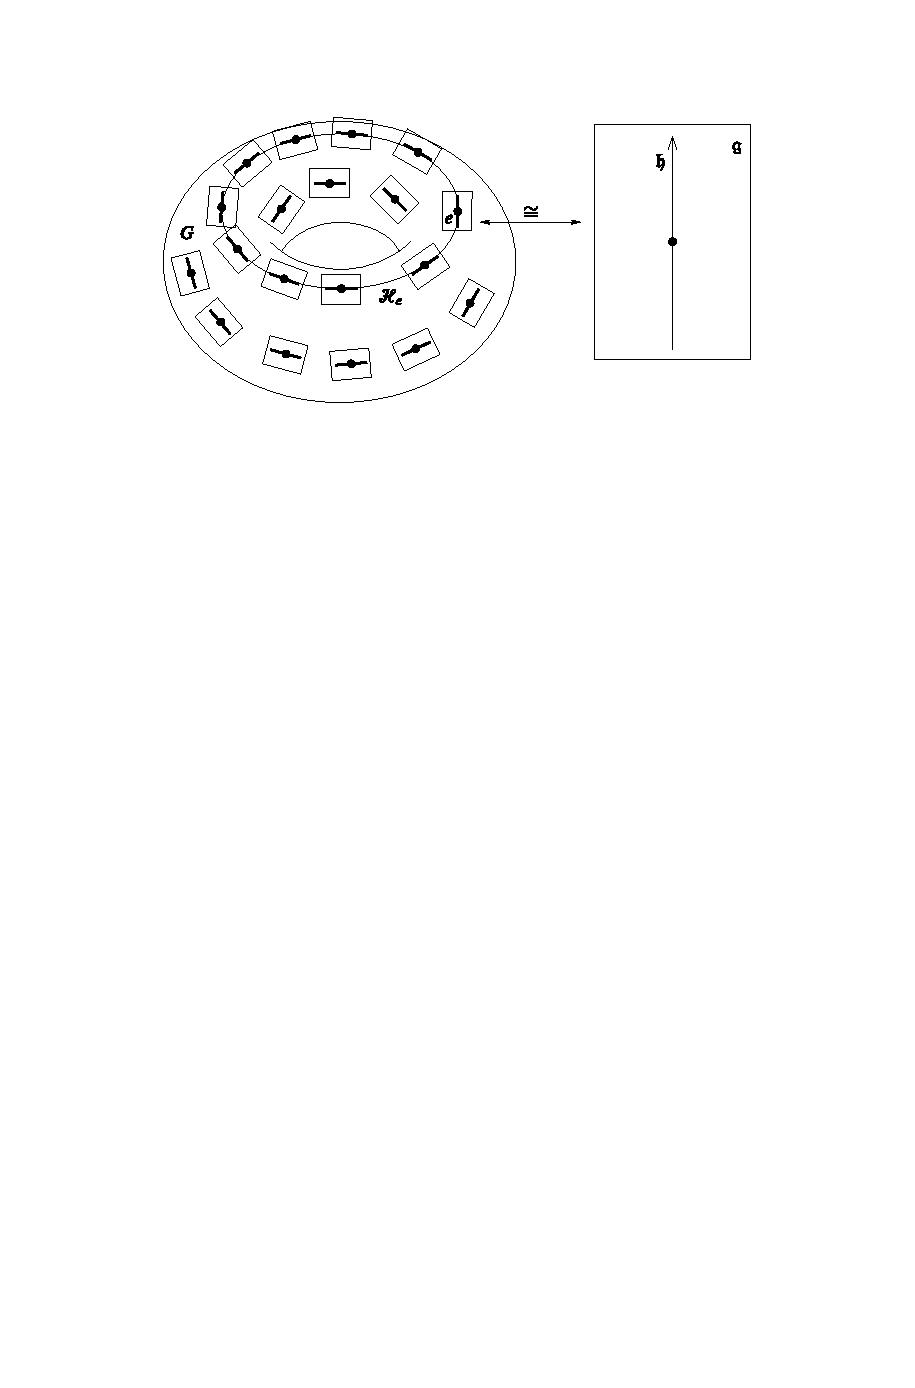
\includegraphics{pictures/Lie-sugroup}
\caption{Finding a subgroup whose Lie algebra is $\h$.}
\end{figure}
\begin{proof}
Suppose $\h$ is a Lie subalgebra of $\g$. Let $D\sub TG$ be the involutive distribution of $\h$. Let $\mathcal{H}$ 
denote the foliation determined by $D$, and for any $g\in G$, let $\mathcal{H}_g$ denote the leaf of $\mathcal{H}$ 
containing $g$. Because $D$ is left-invariant, it follows from Proposition~\ref{distribution invariant} that each 
left translation takes leaves to leaves: for any $g,g'\in G$, we have $L_g(\mathcal{H}_{g'})=\mathcal{H}_{gg'}$.\par
Define $H=\mathcal{H}_e$, the leaf containing the identity. We will show that $H$ is the desired Lie subgroup.\par
First, to see that $H$ is a subgroup, observe that for any $h,h'\in H$,
\[hh'=L_h(h')\in L_h(H)=L_h(\mathcal{H}_e)=\mathcal{H}_h=H.\]
Similarly,
\[h^{-1}=h^{-1}e=L_{h^{-1}}(\mathcal{H}_e)=L_{h^{-1}}(\mathcal{H}_h)=\mathcal{H}_e=H.\]
To show that $H$ is a Lie group, we need to show that the map $\mu:(h,h')\mapsto h^{-1}h'$ is smooth as a map from 
$H\times H$ to $H$. Because $H\times H$ is a submanifold of $G\times G$, it is immediate that $\mu:H\times H\to G$ 
is smooth. Since $H$ is an integral manifold of an involutive distribution, Theorem~\ref{integral mani weak embedd} shows that it is weakly embedded, so $\mu$ is
also smooth as a map into $H$.\par
The fact that $H$ is a leaf of $\mathcal{H}$ implies that the Lie algebra of $H$ is $\h$, because the tangent 
space to $H$ at the identity is $D_e=\{X_e:X\in\h\}$. To see that $H$ is the unique connected subgroup with Lie 
algebra $\h$, suppose $\widetilde{H}$ is any other connected subgroup with the same Lie algebra. Any such Lie 
subgroup is easily seen to be an integral manifold of $D$, so by maximality of $H=\mathcal{H}_e$, we must have 
$\widetilde{H}\sub H$. On the other hand, if $U$ is the domain of a flat chart for $D$ containing the identity, 
then by Proposition~\ref{integral mani local struct}, $\widetilde{H}\cap U$ is a union of open subsets of slices. 
Since the slice containing $e$ is an open subset of $H$, this implies that $\widetilde{H}$ contains a neighborhood 
of the identity in $H$. Since any neighborhood of the identity generates $H$ (Proposition~\ref{topo group prop}), 
this implies that $\widetilde{H}=H$.
\end{proof}
Since nonclosed subgroups can be pathological, Theorem~\ref{Lie subgroup generated by Lie subalgebra} is most useful in cases where the connected Lie subgroup $H$ is actually closed. The following result gives one condition under which this is guaranteed to be the case.
\begin{proposition}\label{Lie subgroup generated by Lie subalgebra closed if maximal abelian}
Suppose $G$ is a Lie group with Lie algebra $\g$ and that $\h$ is a maximal commutative subalgebra of $\g$, meaning that $\h$ is commutative and h is not contained in any larger commutative subalgebra of $\g$. Then the connected Lie subgroup $H$ of $G$ with Lie algebra $\h$ is closed.
\end{proposition}
\begin{proof}
Since $\h$ is commutative, $H$ is also commutative, since every element of $H$ is a product of exponentials of elements of $\h$ (Proposition~\ref{Lie group exp generate}). It easily follows that the closure $\widebar{H}$ of $H$ in $G$ is also commutative. Since $H$ is connected, $\widebar{H}$ is also connected. Now, since $\widebar{H}$ is commutative, its Lie algebra $\h'$ is also commutative. But since $\h$ was maximal commutative, we must have $\h'=\h$. Since, also, $\widebar{H}$ is connected, we conclude that $H=\widebar{H}$, showing that $H$ is closed.
\end{proof}
\subsection{One-parameter subgroups and the exponential map}
Suppose $G$ is a Lie group. Since left-invariant vector fields are naturally defined in terms of the group structure of $G$, one might reasonably expect to find some relationship between the group law for the flow of a left-invariant vector field and
group multiplication in $G$. We begin by exploring this relationship.
\subsubsection{One-Parameter Subgroups}
A \textbf{one-parameter subgroup} of $G$ is defined to be a Lie group homomorphism $\gamma:\R\to G$, with $\R$ considered as a Lie group under addition. By this definition, a one-parameter subgroup is not a Lie subgroup of $G$, but rather a homomorphism into $G$.
\begin{theorem}[\textbf{Characterization of One-Parameter Subgroups}]\label{one-para subgroup char}
Let $G$ be a Lie group. The one-parameter subgroups of $G$ are precisely the maximal integral curves of left-invariant vector fields starting at the identity.
\end{theorem}
\begin{proof}
First suppose $\gamma$ is the maximal integral curve of some left-invariant vector field $X\in\Lie(G)$ starting at the identity. Because left-invariant vector fields are complete (Theorem~\ref{vector field left-inva complete}), $\gamma$ is defined on all of $\R$. Left-invariance means that $X$ is $L_g$-related to itself for every $g\in G$, so $L_g$ takes integral curves of $X$ to integral curves of $X$. Applying this with $g=\gamma(s)$ for some $s\in\R$, we conclude that the curve $t\mapsto L_{\gamma(s)}\big(\gamma(t)\big)$ is an integral curve starting at $\gamma(s)$. But the curve $t\mapsto\gamma(t+s)$ is also an integral curve with the same initial point, so they are equal:
\[\gamma(s)\gamma(t)=\gamma(s+t).\]
This says precisely that $\gamma:\R\to G$ is a one-parameter subgroup.\par
Conversely, suppose $\gamma:\R\to G$ is a one-parameter subgroup, and let $X=\gamma_*(d/dt)\in\Lie(G)$, treating $d/dt$ as a left-invariant vector field on $\R$. Since $\gamma(0)=e$, we just have to show that $\gamma$ is an integral curve of $X$. Recall that $\gamma_*(d/dt)$ is defined as the unique left-invariant vector field on $G$ that is $\gamma_*$-related to $d/dt$ (see Theorem~\ref{Lie algebra induce}). Therefore, for any $t_0\in\R$,
\[\gamma'(t_0)=d\gamma_{t_0}\Big(\frac{d}{dt}\Big|_{t_0}\Big)=X_{\gamma(t_0)}.\]
so $\gamma$ is an integral curve of $X$.
\end{proof}
Given $X\in\Lie(G)$, the one-parameter subgroup determined by $X$ in this way is called the \textbf{one-parameter subgroup generated by $\bm{X}$}. Because left-invariant vector fields are uniquely determined by their values at the identity, it follows that each one-parameter subgroup is uniquely determined by its initial velocity in $T_eG$, and thus there are one-to-one correspondences
\[\text{one-parameter subgroups of $G$}\leftrightarrow\Lie(G)\leftrightarrow T_eG.\]
The one-parameter subgroups of $\GL_n(\R)$ are not hard to compute explicitly.
\begin{proposition}
For any $A\in\gl(n,\R)$, let
\begin{align}\label{exp def gl(n,R)}
e^A=\sum_{k=0}^{\infty}\frac{A^k}{k!}.
\end{align}
This series converges to an invertible matrix $e^A\in\GL_n(\R)$, and the one-parameter subgroup of $\GL_n(\R)$ generated by $A\in\gl(n,\R)$ is $\gamma(t)=e^{tA}$.
\end{proposition}
\begin{proof}
First, we verify convergence. The matrix multiplication satisfies $|AB|\leq|A||B|$, where the norm is the Frobenius norm on $\gl(n,\R)$. It follows by induction that $|A^k|\leq |A|^k$. The Weierstrass $M$-test then shows that $(\ref{exp def gl(n,R)})$ converges uniformly on any bounded subset of $\gl(n,\R)$, by comparison with the series $\sum_{k=0}^{\infty}c^k/k!$.\par
Fix $A\in\gl(n,\R)$. Under our identification of $\gl(n,\R)$ with $\Lie(\GL_n(\R))$, the matrix $A$ corresponds to the left-invariant vector field $A^L$ given by $(\ref{Lie algebra iso-1})$. Thus, the one-parameter subgroup generated by $A$ is an integral curve of $A^L$ on $\GL_n(\R)$, and therefore satisfies the ODE initial value problem
\[\gamma'(t)=A^L|_{\gamma(t)},\quad \gamma(0)=I_n.\]
Using $(\ref{Lie algrbra gl(n,R)})$, the condition for $\gamma$ to be an integral curve can be rewritten as
\[\dot{\gamma}^i_k(t)=\gamma^i_j(t)A^j_k,\]
or in matrix notation
\[\gamma'(t)=\gamma(t)A.\]
We will show that $\gamma(t)=e^{tA}$ satisfies this equation. Since $\gamma(0)=I_n$, this implies that $\gamma$ is the unique integral curve of $A^L$ starting at the identity and is therefore the desired one-parameter subgroup.\par
To see that $\gamma$ is differentiable, we note that differentiating the series $(\ref{exp def gl(n,R)})$ formally term by term yields the result
\[\gamma'(t)=\sum_{k=1}^{\infty}\frac{A^k}{(k-1)!}=\gamma(t)A=A\gamma(t).\]
Since the differentiated series converges uniformly on bounded sets, the term-by-term differentiation is justified. By smoothness of solutions to ODEs, $\gamma$ is a smooth curve.\par
It remains only to show that $\gamma(t)$ is invertible for all $t$, so that $\gamma$ actually takes its values in $\GL_n(\R)$. If we let $\sigma(t)=\gamma(t)\gamma(-t)=e^{tA}e^{-tA}$, then $\sigma$ is a smooth curve in $\gl(n,\R)$, and by the previous computation and the product rule it satisfies
\[\sigma'(t)=\big(\gamma(t)A\big)\gamma(-t)-\gamma(t)\big(A\gamma(-t)\big)=0.\]
It follows that $\sigma$ is the constant curve $\sigma(t)=I_n$, which is to say that
$\gamma(t)=\gamma(-t)^{-1}$. 
\end{proof}
\begin{proposition}\label{one-para Lie subgroup}
Suppose $G$ is a Lie group and $H\sub G$ is a Lie subgroup. The one-parameter subgroups of $H$ are precisely those one-parameter subgroups of $G$ whose initial velocities lie in $T_eH$.
\end{proposition}
\begin{proof}
Let $\gamma:\R\to H$ be a one-parameter subgroup. Then the composite map
\[\begin{tikzcd}
\R\ar[r,"\gamma"]&H\ar[r,hook]&G
\end{tikzcd}\]
is a Lie group homomorphism and thus a one-parameter subgroup of $G$, which clearly satisfies $\gamma'(0)\in T_eH$.\par
Conversely, suppose $\gamma:\R\to G$ is a one-parameter subgroup whose initial velocity lies in $T_eH$. Let $\widetilde{\gamma}:\R\to H$ be the one-parameter subgroup of $H$ with the same initial velocity $\widetilde{\gamma}'(0)=\gamma'(0)\in T_eH\sub T_eG$. As in the preceding paragraph, by composing with the inclusion map, we can also consider $\widetilde{\gamma}$ as a one-parameter subgroup of $G$. Since $\gamma$ and $\widetilde{\gamma}$ are both one-parameter subgroups of $G$ with the same initial velocity, they must be equal.
\end{proof}
\begin{example}
If $H$ is a Lie subgroup of $\GL_n(\R)$, the preceding proposition shows that the one-parameter subgroups of $H$ are precisely the maps of the form $\gamma(t)=e^{tA}$ for $A\in\h$, where $\h\sub\gl(n,\R)$ is the subalgebra corresponding to $\Lie(H)$ as in Theorem~\ref{Lie subalgebra}. For example, taking $H=\O(n)$, this shows that the one-parameter subgroups of $\O(n)$ are the maps of the form $\gamma(t)=e^{tA}$ for an arbitrary skew-symmetric matrix $A$. In particular, this shows that the exponential of any skew-symmetric matrix is orthogonal.
\end{example}
\subsubsection{The Exponential Map}
In the preceding part we saw that the matrix exponential maps $\gl(n,\R)$ to $\GL_n(\R)$ and takes each line through the origin to a one-parameter subgroup. This
has a powerful generalization to arbitrary Lie groups.\par
Given a Lie group $G$ with Lie algebra $\g$, we define a map $\exp:\g\to G$, called the \textbf{exponential map of $\bm{G}$}, as follows: for any $X\in\g$, we set
\[\exp(X)=\gamma(1),\]
where $\gamma$ is the one-parameter subgroup generated by $X$, or equivalently the integral curve of $X$ starting at the identity. The following proposition shows that,
like the matrix exponential, this map sends the line through $X$ to the one-parameter
subgroup generated by $X$.
\begin{proposition}[\textbf{(One-Parameter Subgroups}]\label{exp map one-para}
Let $G$ be a Lie group. For any $X\in\Lie(G)$, $\gamma(t)=\exp tX$ is the one-parameter subgroup of $G$ generated by $X$.
\end{proposition}
\begin{figure}[htbp]
\centering
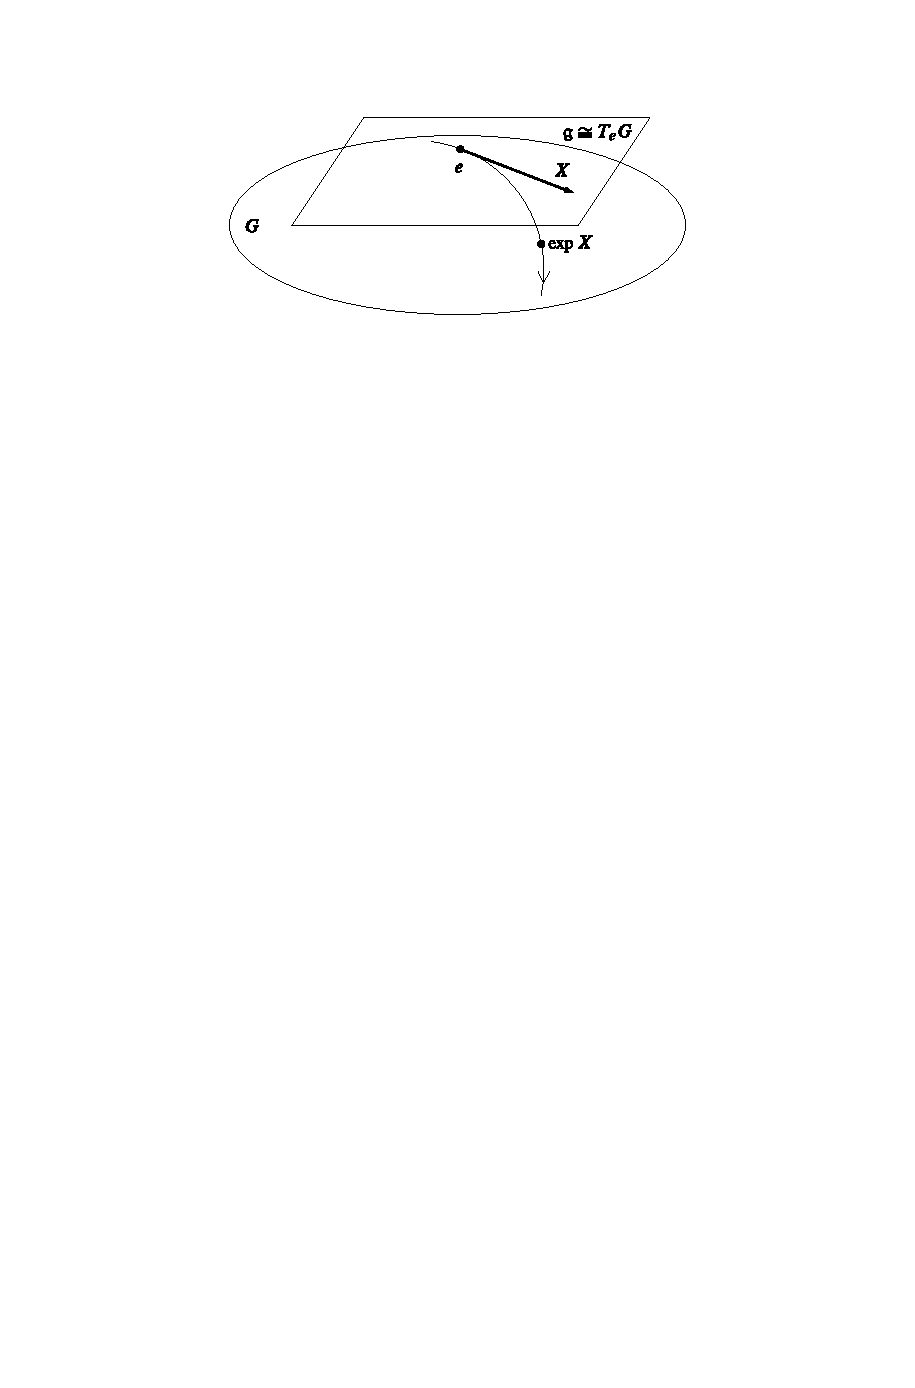
\includegraphics{pictures/exp-map}
\caption{The exponential map.}
\end{figure}
\begin{proof}
Let $\gamma:\R\to G$ be the one-parameter subgroup generated by $X$, which is the integral curve of $X$ starting at $e$. For any fixed $t\in\R$, it follows from the rescaling lemma 
that $\widetilde{\gamma}(s)=\gamma(ts)$ is the integral curve of $tX$ starting at $e$, so
\[\exp tX=\widetilde{\gamma}(1)=\gamma(t)\]
as needed.
\end{proof}
Here are two simple but important examples.
\begin{example}
The results of the preceding part show that the exponential map of $\GL_n(\R)$ (or any Lie subgroup of it) is given by $\exp A=e^A$. This, obviously, is the reason for the term exponential map.
\end{example}
\begin{example}
If $V$ is a finite-dimensional real vector space, a choice of basis for $V$ yields isomorphisms $\GL(V)\cong\GL_n(\R)$ and $\gl(V)\cong\gl(n,\R)$. The analysis of the $\GL_n(\R)$ case then shows that the exponential map of $\GL(V)$ can be written in
the form 
\[\exp A=\sum_{k=0}^{\infty}\frac{A^k}{k!},\]
where we consider $A\in\gl(V)$ as a linear map from $V$ to itself, and $A^k=A\circ\cdots\circ A$ is the $k$-fold composition of $A$ with itself.
\end{example}
\begin{proposition}[\textbf{Properties of the Exponential Map}]\label{Lie group exp prop}
Let $G$ be a Lie group and let $\g$ be its Lie algebra.
\begin{itemize}
\item[(a)] The exponential map is a smooth map from $\g$ to $G$.
\item[(b)] For any $X\in\g$ and $s,t\in\R$, $\exp(s+t)X=\exp sX\exp tX$.
\item[(c)] For any $X\in\g$, $(\exp X)^{-1}=\exp(-X)$.
\item[(d)] For any $X\in\g$ and $n\in\Z$, $(\exp X)^n=\exp(nX)$.
\item[(e)] The differential $(d\exp)_0:T_0\g\to T_eG$ is the identity map, under the canonical identifications of both $T_0\g$ and $T_eG$ with $\g$ itself.
\item[(f)] The exponential map restricts to a diffeomorphism from some neighborhood of $0$ in $\g$ to a neighborhood of $e$ in $G$.
\item[(g)] If $H$ is another Lie group, $\h$ is its Lie algebra, and $\varPhi:G\to H$ is a Lie group homomorphism, the following diagram commutes:
\[\begin{tikzcd}
\g\ar[r,"\varPhi_*"]\ar[d,swap,"\exp"]&\h\ar[d,"\exp"]\\
G\ar[r,"\varPhi"]&H
\end{tikzcd}\]
\item[(h)] The flow $\theta$ of a left-invariant vector field $X$ is given by $\theta_t=R_{\exp tX}$ $($right multiplication by $\exp tX$$)$.
\end{itemize}
\end{proposition}
\begin{figure}[htbp]
\centering
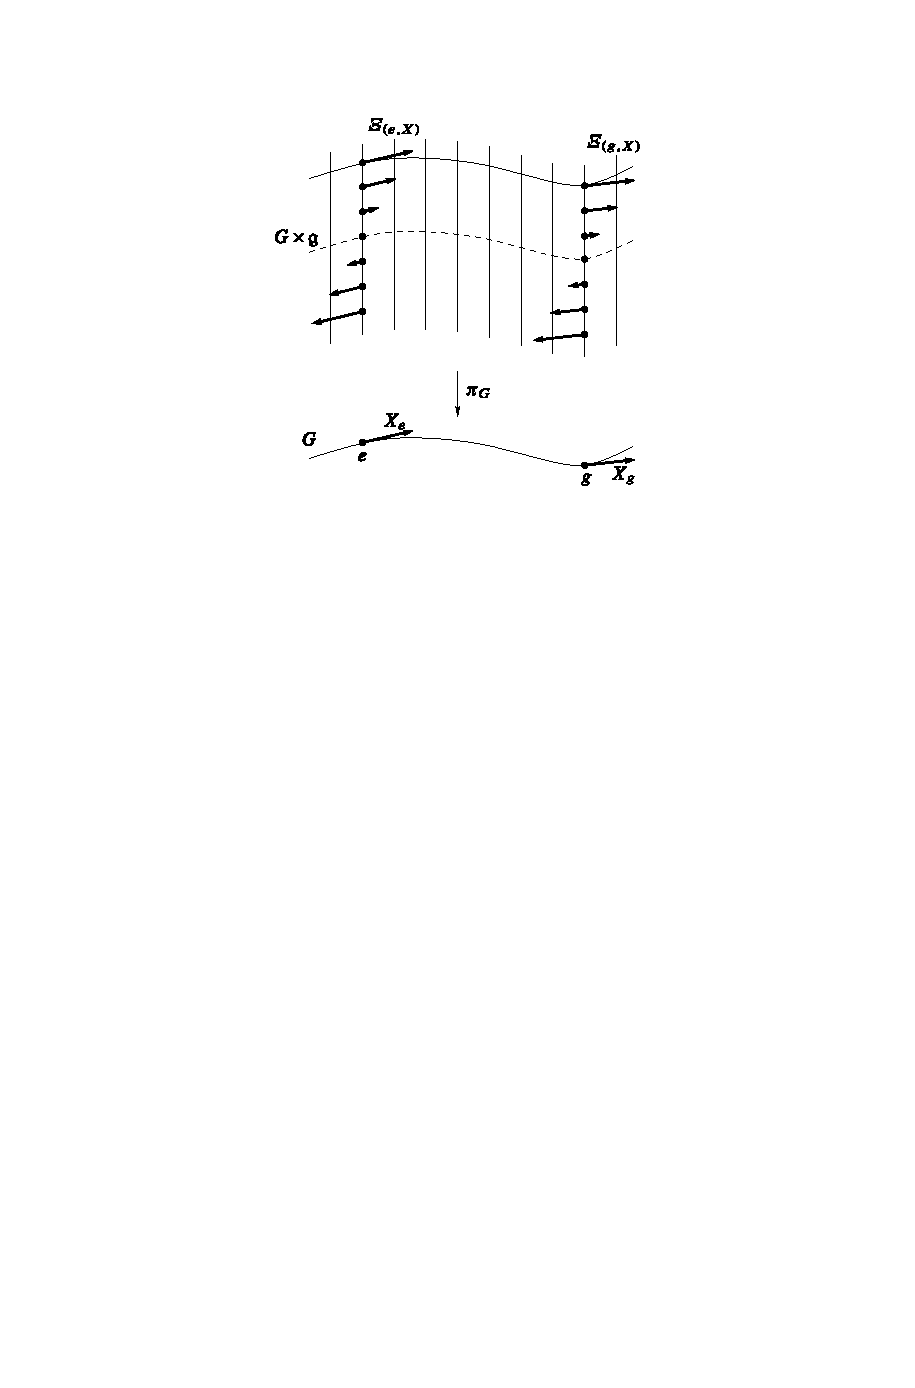
\includegraphics{pictures/exp-map-prop}
\caption{Proof that the exponential map is smooth.}
\end{figure}
\begin{proof}
In this proof, for any $X\in\g$ we let $\theta_X$ denote the flow of $X$. To prove (a), we need to show that the expression $\theta_X^{(e)}(1)$ depends smoothly on $X$, which amounts to showing that the flow varies smoothly as the vector field varies. This is a situation not covered by the fundamental theorem on flows, but we can reduce it to that theorem by the following simple trick. Define a vector field $\varXi$ on the product manifold $G\times\g$ by
\[\varXi_{(g,X)}=(X_g,0)\in T_gG\oplus T_X\g\cong T_{(g,X)}(G\times\g).\]
To see that $\varXi$ is a smooth vector field, choose any basis $(X_1,\dots,X_k)$ for $\g$, and let $(x^i)$ be the corresponding global coordinates for $\g$, defined by $(x^i)\leftrightarrow x^iX_i$. Let $(w^i)$ be any smooth local coordinates for $G$. If $f\in C^\infty(G\times\g)$ is arbitrary, then locally we can write
\[\varXi f(w^i,x^i)=x^jX_jf(w^i,x^i),\]
where each vector field $X_j$ differentiates $f$ only in the $w^i$-directions. Since this depends smoothly on $(w^i,x^i)$, it follows from Proposition~\ref{vector field smooth by function} that $\varXi$ is smooth. It is easy to verify that the flow $\varTheta$ of $\varXi$ is given by
\[\varTheta_t(g,X)=(\theta_X(t,g),X).\]
By the fundamental theorem on flows, $\varTheta$ is smooth. Since $\exp X=\pi_G\big(\varTheta_1(e,X)\big)$, where $\pi_G:G\times\g\to G$ is the projection, it follows that $\exp$ is smooth.\par
Next, (b) and (c) follow immediately from Proposition~\ref{exp map one-para}, because $t\mapsto\exp tX$ is a group homomorphism from $\R$ to $G$. Then (d) for nonnegative $n$ follows from (b) by induction, and for negative $n$ it follows from (c).\par
To prove (e), let $X\in\g$ be arbitrary, and let $\sigma:\R\to\g$ be the curve $\sigma(t)=tX$. Then $\sigma'(0)=X$, and Proposition~\ref{exp map one-para} implies
\[(d\exp)_0(X)=(d\exp)_0\big(\sigma'(0)\big)=(\exp\circ\sigma)'(0)=\frac{d}{dt}\Big|_{t=0}\exp tX=X.\]
Part (f) then follows immediately from (e) and the inverse function theorem.\par
Next, to prove (g) we need to show that $\exp(\varPhi_*X)=\varPhi(\exp X)$ for every $X\in g$. In fact, we will show that for all $t\in\R$,
\[\exp(t\varPhi_*X)=\varPhi(\exp tX).\]
The left-hand side is, by Proposition~\ref{exp map one-para}, the one-parameter subgroup generated by $\varPhi_*X$. Thus, if we put $\sigma(t)=\varPhi(\exp tX)$, it suffices to show that $\sigma:\R\to H$ is a Lie group homomorphism satisfying $\sigma'(0)=(\varPhi_*X)_e$. It is a Lie group homomorphism because it is the composition of the homomorphisms $\varPhi$ and $t\mapsto\exp tX$. The initial
velocity is computed as follows:
\[\sigma'(0)=\frac{d}{dt}\Big|_{t=0}\varPhi(\exp tX)=d\varPhi_e\Big(\frac{d}{dt}\Big|_{t=0}\exp tX\Big)=d\varPhi_e(X_e)=(\varPhi_* X)_e.\]

Finally, to show that $(\theta_X)_t=R_{\exp tX}$, we use the fact that for any $g\in G$, the left multiplication map $L_g$ takes integral curves of $X$ to integral curves of $X$. Thus, the map $t\mapsto L_g(\exp tX)$ is the integral curve starting at $g$, which means it is equal to $\theta_X^{(g)}(t)$. It follows that
\[R_{\exp tX}(g)=g\exp tX=L_g(\exp tX)=\theta_X^{(g)}(t)=(\theta_X)_t(g).\]
This completes the proof.
\end{proof}
The exponential map yields the following alternative characterization of the Lie subalgebra of a subgroup.We will use this later when we study normal subgroups.
\begin{proposition}\label{Lie subalgebra exp}
Let $G$ be a Lie group, and let $H\sub G$ be a Lie subgroup. With $\Lie(H)$ considered as a subalgebra of $\Lie(G)$ in the usual way, the exponential map of $H$ is the restriction to $\Lie(H)$ of the exponential map of $G$, and
\[\Lie(H)=\{X\in\Lie(G):\exp tX\in H\text{ for all $t\in\R$}\}.\]
\end{proposition}
\begin{proof}
The fact that the exponential map of $H$ is the restriction of that of $G$ is an immediate consequence of Proposition~\ref{one-para Lie subgroup}. To prove the second assertion, by the way we have identified $\Lie(H)$ as a subalgebra of $\Lie(G)$, we need to establish the following equivalence for every $X\in\Lie(G)$:
\[\exp tX\in H\text{ for all $t\in\R$}\iff X_e\in T_eH.\]
Assume first that $\exp tX\in H$ for all $t$. Since $H$ is weakly embedded in $G$ by
Theorem~\ref{Lie subgroup weak embedd}, it follows that the curve $t\mapsto\exp tX$ is smooth as a map into $H$, and thus $X_e=\gamma'(0)\in T_eH$. Conversely, if $X_e\in T_eH$, then Proposition~\ref{one-para Lie subgroup} implies that $\exp tX\in H$ for all $t$.
\end{proof}
Notice that Proposition~\ref{Lie group exp prop}(d) does not imply $\exp(X+Y)=(\exp X)(\exp Y)$ for arbitrary $X,Y$ in the Lie algebra. In fact, for connected groups, this is true only when the group is abelian.
\begin{proposition}\label{Lie group exp generate}
If $G$ is a connected Lie group, then $G$ is generated by the image of the exponential map.
\end{proposition}
\begin{proof}
This comes from the fact that if $G$ is a connected topological group, then it is generated by any neighborhood of the identity (Proposition~\ref{topo group prop}).
\end{proof}
\begin{example}
Let $G=\SO(3)$. Then $\g=\so(3)$ consists of skew-symmetric $3\times 3$ matrices. One possible choice of a basis in $\so(3)$ is
\[J_x=\begin{pmatrix}
0&0&0\\
0&0&-1\\
0&1&0
\end{pmatrix}\quad J_y=\begin{pmatrix}
0&0&1\\
0&0&0\\
-1&0&0
\end{pmatrix}\quad J_z=\begin{pmatrix}
0&1&0\\
-1&0&0\\
0&0&0
\end{pmatrix}\]
We can explicitly describe the corresponding subgroups in $G$. Namely,
\[\exp(tJ_x)=\begin{pmatrix}
1&0&0\\
0&\cos t&-\sin t\\
0&\sin t&\cos t
\end{pmatrix}\]
is rotation around $x$-axis by angle $t$; similarly, $J_y$, $J_z$ generate rotations around $y,z$ axes. The easiest way to show this is to note that such rotations do form a one-parameter subgroup; thus, they must be of the form $\exp(tJ)$ for some $J\in\so(3)$, and then compute the derivative to find $J$.\par
By Theorem~\ref{Lie group exp generate}, elements of the form $\exp(tJ_x),\exp(tJ_y),\exp(tJ_z)$ generate $\SO(3)$. For this reason, it is common to refer to $J_x,J_y,J_z$ as "infinitesimal generators" of $\SO(3)$. Thus, in a certain sense $\SO(3)$ is generated by three elements.
\end{example}
\begin{corollary}\label{Lie group homo is uniquely determined by algebra homo}
Let $G$ and $H$ be Lie groups with Lie algebras $\g$ and $\h$, respectively, and assume $G$ is connected. Then any Lie group homomorphism $\varPhi:G\to H$ is uniquely determined by $\varPhi_*:\g\to\h$.
\end{corollary}
\begin{proof}
Let $g$ be any element of $G$. Since $G$ is connected, Corollary~\ref{Lie group exp generate} tells us that every element of $G$ can be written as $\exp(x_1)\cdots\exp(X_m)$, with $X_i\in\g$. Let $\varphi=\varPhi_*$, then by Proposition~\ref{Lie group exp prop},
\begin{align*}
\varPhi(g)&=\varPhi_1(\exp(x_1)\cdots\exp(X_m))=\exp(\phi(X_1))\cdots\exp(\phi(X_m)).
\end{align*}
Therefore $\varPhi$ is determined by $\varphi$.
\end{proof}
\begin{corollary}\label{Lie group abelian algebra}
Let $G$ be a Lie group and $\g$ be its Lie algebra. If $G$ is abelian, then $\g$ is commutative. The converse holds if $G$ is connected.
\end{corollary}
\begin{proof}
If $G$ is abelian, then the inverse map $i:G\to G$ is a Lie group homomorphism, therefore by By Exercise~\ref{Lie group operator diff},
\[-[X,Y]=i_*[X,Y]=[i_*X,i_*Y]=[di_e(X),di_e(Y)]=[-X,-Y]=[X,Y]\]
for any $X,Y\in\g$. This implies that $\g$ is commutative.\par
Conversely, if $G$ is connected then any element of $G$ can be written as in Corollary~\ref{Lie group exp generate}. Thus by Proposition~\ref{Lie group commuting vector field exp}, $G$ abelian.
\end{proof}
\subsection{The closed subgroup theorem}
Recall that in Theorem~\ref{Lie subgroup closed iff embed} we showed that a Lie subgroup is embedded if and only if it is closed. In this section, we use the exponential map to prove a much stronger form of that theorem, showing that if a subgroup of a Lie group is topologically a closed subset, then it is actually an embedded Lie subgroup.\par
We begin with a simple result that shows how group multiplication in $G$ is reflected to first order in the vector space structure of its Lie algebra.
\begin{proposition}\label{Lie group commuting vector field exp}
Let $G$ be a Lie group and $\g$ be its Lie algebra. Let $X,Y\in\g$ be such that $[X,Y]=0$. Then
\[(\exp X)(\exp Y)=\exp(X+Y)=(\exp Y)(\exp X).\]
\end{proposition}
\begin{proof}
Let $\theta_X$ and $\theta_Y$ be the flows determined by $X$ and $Y$, respectively. Since $[X,Y]=0$, these two flows commute. Therefore
\[\theta_X(t)\theta_Y(s)\theta_X(-t)=\theta_Y(s).\]
Applying this at $e\in G$ and using Proposition~\ref{Lie group exp prop}(h), we then get
\[(\exp tX)(\exp sY)(\exp(-tX))=\exp sY.\]
So $\exp tX,\exp sY$ commute for all values of $s,t$. In particular, this implies $(\exp tX)(\exp tY)$ is a one-parameter subgroup; computing the tangent vector at $t=0$, we see that 
\[(\exp tX)(\exp tY)=\exp(t(X+Y)).\]
Evaluating at $t=1$ gives the claim.
\end{proof}
\begin{proposition}
Let $G$ be a Lie group and let $\g$ be its Lie algebra. For any $X,Y\in\g$, there is a smooth function $Z:(-\eps,\eps)\to\g$ for some $\eps>0$ such that the following identity holds for all $t\in(-\eps,\eps)$:
\begin{align}\label{Lie algebra first order-1}
(\exp tX)(\exp tY)=\exp\big(t(X+Y)+t^2Z(t)\big).
\end{align}
\end{proposition}
\begin{proof}
Since the exponential map is a diffeomorphism on some neighborhood of the origin in $\g$, there is some $\eps>0$ such that the map $\varphi:(-\eps,\eps)\to\g$ defined by
\[\varphi(t)=\exp^{-1}(\exp tX\exp tY)\]
is smooth. It obviously satisfies $\varphi(0)=0$ and 
\[\exp tX\exp tY=\exp\varphi(t).\]
Observe that we can write $\varphi$ as the composition
\[\begin{tikzcd}
\R\ar[r,"e_X\times e_Y"]&G\times G\ar[r,"m"]&G\ar[r,"\exp^{-1}"]&\g
\end{tikzcd}\]
where $e_X(t)=\exp tX$ and $e_Y(t)=\exp tY$. The result of Exercise~\ref{Lie group operator diff} shows that $dm_{(e,e)}(X,Y)=X+Y$ for $X,Y\in T_eG$, which implies
\[\varphi'(0)=\big((d\exp)_0\big)^{-1}(e_X'(0)+e_Y'(0))=X+Y.\]
Therefore, Taylor's theorem yields
\[\varphi(t)=t(X+Y)+t^2Z(t)\]
for some smooth function $Z$.
\end{proof}
\begin{corollary}
Under the hypotheses of the preceding proposition,
\begin{align}\label{Lie algebra first order-2}
\lim_{n\to\infty}\Big(\Big(\exp\frac{t}{n}X\Big)\Big(\exp\frac{t}{n}Y\Big)\Big)^n=\exp t(X+Y).
\end{align}
\end{corollary}
\begin{proof}
Formula $(\ref{Lie algebra first order-1})$ implies that for any $t\in\R$ and any sufficiently large $n\in\Z$,
\[\Big(\exp\frac{t}{n}X\Big)\Big(\exp\frac{t}{n}Y\Big)=\exp\Big(\frac{t}{n}(X+Y)+\frac{t^2}{n^2}Z\Big(\frac{t}{n}\Big)\Big),\]
and then Proposition~\ref{Lie group exp prop}(d) yields
\[\Big(\Big(\exp\frac{t}{n}X\Big)\Big(\exp\frac{t}{n}Y\Big)\Big)^n=\exp\Big(t(X+Y)+\frac{t^2}{n}Z\Big(\frac{t}{n}\Big)\Big).\]
Fixing $t$ and taking the limit as $n\to\infty$, we obtain $(\ref{Lie algebra first order-2})$.
\end{proof}
\begin{theorem}[\textbf{Closed Subgroup Theorem}]\label{Lie closed subgroup}
Suppose $G$ is a Lie group and $H\sub G$ is a closed subgroup of $G$. Then $H$ is an embedded Lie subgroup.
\end{theorem}
\begin{proof}
By Proposition~\ref{Lie subgroup embedd mani}, it suffices to show that $H$ is an embedded submanifold of $G$. We begin by identifying a subspace of $\Lie(G)$ that will turn out to be the Lie algebra of $H$.\par
Let $\g=\Lie(G)$, and define a subset $\h\sub\g$ by
\[\h=\{X\in\g:\exp tX\in H\text{ for all }t\in\R\}.\]
We need to show that $\h$ is a linear subspace of $\g$. It is obvious from the definition that $\h$ is closed under scalar multiplication: if $X\in\h$, then $tX\in\h$ for all $t\in R$. Suppose $X,Y\in\h$, and let $t\in\R$ be arbitrary. Then $\exp\big((t/n)X\big)$ and $\exp\big((t/n)Y\big)$ are in $H$ for each positive integer $n$, and because $H$ is a closed subgroup of $G$, $(\ref{Lie algebra first order-2})$ implies that $\exp t(X+Y)\in H$. Thus $X+Y\in\h$, so $\h$ is a subspace.\par
Next we show that there is a neighborhood $U$ of the origin in $\g$ on which the
exponential map of $G$ is a diffeomorphism, and which has the property that
\begin{align}\label{Lie closed subgroup-1}
\exp(U\cap\h)=(\exp U)\cap H.
\end{align}
Note that, by the definition of $\h$ we already have $\exp(U\cap\h)\sub(\exp U)\cap H$, so we only need to show that $U$ can be chosen small enough that $(\exp U)\cap H\sub\exp(U\cap\h)$. Assume this is not possible.\par
Take a vector subspace $\h'$ of $\g$ so that $\g=\h\oplus\h'$. Let $\varPhi:\g=\h\oplus\h'\to G$ be the map
\[\varPhi(X,Y)=\exp X\exp Y.\]
By the result of Exercise~\ref{Lie group operator diff}, $d\varPhi_0(X,Y)=X+Y$, so $\varPhi$ is a diffeomorphism in some neighborhood of $(0,0)$. Choose neighborhoods $U_0$ of $0$ in $\g$ and $\widetilde{U}_0$ of $(0,0)$ in $\h\oplus\h'$ such that both $\exp|_{U_0}$ and $\varPhi|_{\widetilde{U}_0}$ are diffeomorphisms onto their images. Let $\{U_i\}$ be a countable neighborhood basis for $\g$ at $0$. If we set $V_i=\exp(U_i)$ and $\widetilde{U}_i=\varPhi^{-1}(V_i)$, then and are neighborhood bases for $G$ at $e$ and $\h\oplus\h'$ at $(0,0)$, respectively. We may assume that $U_i\sub U_0$ and $\widetilde{U}_i\sub\widetilde{U}_0$ for each $i$.\par
Our assumption implies that for each $i$, there exists $h_i\in(\exp U_i)\cap H$ such that $h_i\notin\exp(U_i\cap\h)$. This means $h_i=\exp Z_i$ for $Z_i\in U_i$. Because $\exp(U_i)=\varPhi(\widetilde{U}_i)$, we can also write
\[h_i=\exp X_i\exp Y_i\]
for $(X_i,Y_i)\in\widetilde{U}_i$. If $Y_i=0$, then $\exp X_i=\exp Z_i$; but $\exp$ is bijective on $U_0$, this implies $X_i=Z_i\in U_i\cap\h$, which
contradicts our assumption that $h_i\notin\exp(U_i\cap\h)$. Observe that $Y_i\to 0$ and $\exp Y_i=(\exp X_i)^{-1}h_i\in H$.\par
Choose an inner product on $\h'$ and let $|\cdot|$ denote the norm associated with this inner product. If we define $c_i=|Y_i|$, then $c_i\to 0$. Consider the sequence $Y_i/|Y_i|$, which lies on the unit sphere in $\h'$. By replacing it by a subsequence, we may assumeso that $\lim_{n\to\infty}Y_i/|Y_i|=Y$, with $|Y|=1$ by continuity. We will show that $\exp tY\in H$ for all $t\in\R$, which implies $Y\in\h$. Since $\h\cap\h'=0$, this is a contradiction.\par
Let $t\in\R$ and set $n_i=[\frac{t}{c_i}]$, so that
\[\Big|n_i-\frac{t}{c_i}\Big|\leq 1,\]
Then $|n_ivc_i-t|\leq c_i\to 0$, implies $n_i|Y_i|\to t$. Thus,
\[\lim_{n\to\infty}\exp(n_iY_i)=\lim_{n\to\infty}\exp(n_ic_i\frac{Y_i}{c_i})=\exp(tY).\]
But $\exp(n_iY_i)=(\exp Y_i)^{n_i}\in H$, so the fact that $H$ is closed implies $\exp tY\in H$. This completes the proof of the existence of $U$ satisfying $(\ref{Lie closed subgroup-1})$.\par
Choose any linear isomorphism $E:\g\to\R^m$ that sends $\h$ to $\R^k$. The composite
map $\varphi=E\circ\exp^{-1}:\exp(U)\to\R^m$ is then a smooth chart for $G$, and $\varphi\big((\exp U)\cap H\big)=E(U\cap\h)$ is the slice obtained by setting the last $m-k$ coordinates equal to zero. Moreover, if $h\in H$ is arbitrary, the left translation map $L_h$ is a diffeomorphism from $\exp U$ to a neighborhood of $h$. Since $H$ is a subgroup, $L_h(H)=H$, and so
\[L_h\big((\exp U)\cap H\big)=L_h(\exp U)\cap H.\]
and $\varphi\circ L_h^{-1}$ is easily seen to be a slice chart for $H$ in a neighborhood of $h$. Thus, $H$ is an embedded submanifold of $G$, hence a Lie subgroup.
\end{proof}
\begin{corollary}
If $G$ is a Lie group and $H$ is any subgroup of $G$, the following are equivalent:
\begin{itemize}
\item[(\rmnum{1})] $H$ is closed in $G$.
\item[(\rmnum{2})] $H$ is an embedded submanifold of $G$.
\item[(\rmnum{3})] $H$ is an embedded Lie subgroup of $G$.
\end{itemize}
\end{corollary}
\begin{proposition}\label{Lie continuous homo smooth}
Every continuous homomorphism of Lie groups is smooth.
\end{proposition}
\begin{proof}
Let $\varphi:G\to H$ be a continuous homomorphism, then 
\[\Gamma_{\varphi}=\{(g,\varphi(g)):g\in G\}\]
is a closed subgroup, and hence a Lie subgroup of $G\times H$. Consider the projection $p:\Gamma_\varphi\to G$ given by the compositoin:
\[\begin{tikzcd}
\Gamma_\varphi\ar[r,hook]&G\times H\ar[r,"\pi_G"]&G
\end{tikzcd}\]
Then $p$ is a bijective, smooth Lie group homomorphism, and a diffeomorphism by Corollary~\ref{Lie isomorphism iff}. Thus $\varphi=\pi_2\circ p^{-1}$ is smooth.
\end{proof}
\begin{corollary}\label{Lie group struct unique}
Let $G$ be a Lie group, then with the given topology, there is only one smooth
structure that makes $G$ into a Lie group.
\end{corollary}
\begin{proof}
Let $\widetilde{G}$ denote the same set $G$ with the same topology, but a different smooth structure such that $G$ is a Lie group. Then the identity map $\mathrm{id}:G\to\widetilde{G}$ is a continuous homomorphism, hence smooth by Proposition~\ref{Lie continuous homo smooth}. Similarly, the map $\mathrm{id}^{-1}:\widetilde{G}\to G$ is also smooth, thus $\mathrm{id}$ is a diffeomorphism. This implies the smooth structure on $G$ and $\widetilde{G}$ coincide.
\end{proof}
Now suppose $S$ is a Lie subgroup of $G$, which is only immersed by our definition. Then by Proposition~\ref{topo subgroup closure} the closure $\widebar{S}$ is also a subgroup, and Theorem~\ref{Lie closed subgroup} says it is embedded. Thus we have the following result.
\begin{proposition}
Suppose $G$ is a Lie group, then every Lie subgroup of $G$ is either a properly embedded submanifold of $G$, or a dense subset of a properly embedded submanifold.
\end{proposition}
\subsection{Infinitesimal generators of group actions}
We have showed that a complete vector field on a manifold generates an action of $\R$ on the manifold. In this part, using the Frobenius theorem and properties of the exponential map, we show how to generalize this notion to actions of higher-dimensional groups.\par
To begin, we need to specify what we mean by an "infinitesimal generator" of a Lie group action. For reasons that will become apparent, in this section we work primarily with right actions. Because $\R$ is abelian, global flows can be considered either as left actions or as right actions, so everything in this part applies to global flows without modification.\par
Suppose we are given a smooth right action of a Lie group $G$ on a smooth manifold $M$; which we denote either by $\theta:M\times G\to M$ or $(p,g)\mapsto p\cdot g$, depending on context. Each element $X\in\mathfrak{Lie}(G)$ determines a smooth global flow on $M$:
\[(t,p)\mapsto p\cdot \exp tX.\]
Let $\widehat{X}\in\X(M)$ be the infinitesimal generator of this flow, so for each $p\in M$,
\begin{align}\label{infinitesimal generator}
\widehat{X}_p=\frac{d}{dt}\Big|_{t=0}p\cdot\exp tX.
\end{align}
Thus we obtain a map $\widehat{\theta}:\mathfrak{Lie}(G)\to\X(M)$, defined by $\widehat{\theta}(X)=\widehat{X}$.\par
There is a useful alternative characterization of $\widehat{X}$ in terms of the orbit map $\theta^{(p)}:G\to M$ defined by $\theta^{(p)}(g)=p\cdot g$. Since $\gamma(t)=\exp tX$ is a smooth curve in $G$ whose initial velocity is $\gamma'(0)=X_e$, it follows from Corollary~\ref{compute diff by curve} that for each $p\in M$ we have
\begin{align}\label{infinitesimal generator diff of orbit map}
 d(\theta^{(p)})_e(X_e)=(\theta^{(p)}\circ\gamma)'=\frac{d}{dt}\Big|_{t=0}p\cdot\exp tX=\widehat{X}_p.
\end{align}
The following result is thus immediate.
\begin{proposition}\label{infinitesimal generator is orbit map related}
Suppose $G$ is a Lie group and $\theta$ is a smooth right action of $G$ on a smooth manifold $M$. For any $X\in\mathfrak{Lie}(G)$ and $p\in M$, the vector fields $X$ and $\widehat{X}$ are $\theta^{(p)}$-related.
\end{proposition}
\begin{proof}
Let $X\in\mathfrak{Lie}(G)$ and $p\in M$ be arbitrary, and write $\widehat{X}=\widehat{\theta}(X)$. Note that the group law $p\cdot gg'=(p\cdot p)\cdot p'$ translates to
\begin{align}\label{infinitesimal generator is orbit map related-1}
\theta^{(p)}\circ L_g(g')=\theta^{(p\cdot g)}(g')
\end{align}
Let $g\in G$ be arbitrary, and write $q=\theta^{(p)}(g)$. Then $(\ref{infinitesimal generator is orbit map related})$ yields $\theta^{(p)}\circ L_g=\theta^{(q)}$. Using this together with $(\ref{infinitesimal generator})$ and the fact that $X$ is left-invariant, we obtain
\[X_q=d(\theta^{(q)})_e(X_e)=d(\theta^{(p)}\circ L_g)_e(X_e)=d(\theta^{(p)})_g\circ d(L_g)_e(X_e)=d(\theta^{(p)})_g(X_g).\]
which proves the claim.
\end{proof}
\begin{proposition}
Suppose $G$ is a Lie group and $\theta$ is a smooth right action of $G$ on a smooth manifold $M$. Then the map $\widehat{\theta}:\mathfrak{Lie}(G)\to\X(M)$ defined above is a Lie algebra homomorphism.
\end{proposition}
\begin{proof}
For each $p\in M$, it follows from $(\ref{infinitesimal generator diff of orbit map})$ that $\widehat{X}_p$ depends linearly on $X$, so $\widehat{\theta}$ is a linear map. Given $p\in M$, Proposition~\ref{infinitesimal generator is orbit map related} together with the naturality of Lie brackets implies that $[X,Y]$ is $\theta^{(p)}$-related to $[\widehat{X},\widehat{Y}]$. This means, in particular, that
\[[\widehat{X},\widehat{Y}]_p=d(\theta^{(p)})_e([X,Y]_e)=\widehat{[X,Y]}_e.\]
Since every point of $M$ is in the image of some orbit map, we conclude that $[\widehat{\theta}(X),\widehat{\theta}(Y)]=\widehat{\theta}([X,Y])$, as claimed.
\end{proof}
The Lie algebra homomorphism $\widehat{\theta}:\mathfrak{Lie}(G)\to\X(M)$ defined above is known as the \textbf{infinitesimal generator} of $\theta$. More generally, if $\g$ is an arbitrary finitedimensional Lie algebra, any Lie algebra homomorphism $\widehat{\theta}:\g\to\X(M)$ is called a \textbf{(right) $\g$-action} on $M$. A $\g$-action $\widehat{\theta}$ is said to be \textbf{complete} if for every $X\in\g$, the
vector field $\widehat{\theta}(X)$ is complete.\par
Just as every complete vector field generates an $\R$-action, the next theorem shows that, at least for simply connected groups, every complete Lie algebra action generates a Lie group action.
\begin{theorem}[\textbf{Fundamental Theorem on Lie Algebra Actions}]\label{Lie group action generated by infinitesimal}
Let $M$ be a smooth manifold, let $G$ be a simply connected Lie group, and let $\g=\mathfrak{Lie}(G)$. Suppose $\widehat{\theta}:\g\to\X(M)$ is a complete $\g$-action on $M$. Then there is a unique smooth right $G$-action on $M$ whose infinitesimal generator is $\widehat{\theta}$.
\end{theorem}
\begin{proof}
We begin by defining a distribution $D$ on $G\times M$; we will show that $D$ is involutive, and then each leaf will turn out to be the graph of an orbit map $\theta^{(p)}:G\to M$. For brevity, given $X\in g$, we use the notation $\widehat{X}$ for $\widehat{\theta}(X)\in\X(M)$.\par
Define $D$ as follows: for each $X\in\g$, define a smooth vector field $\widetilde{X}$ on $G\times M$ by
\[\widetilde{X}_{(g,p)}=(X_g,\widehat{X}_p)\in T_gG\oplus T_pM\cong T_{(g,p)}(G\times M).\]
In the notation of Exercise~\ref{vector field direct sum}, this is $X\oplus\widehat{X}$. Then for each $(g,p)\in G\times M$, let $D_{(g,p)}$ be the set of all vectors of the form $\widetilde{X}$ as $X$ ranges over $\g$. If $X_1,\dots,X_k$ is a basis for $\g$, then the smooth vector fields $\widetilde{X}_1,\dots,\widetilde{X}_k$ are independent and span $D$, so $D$ is a smooth distribution whose rank is equal to the dimension of $G$. To see that it is involutive, note that Exercise~\ref{vector field direct sum} and the fact that $\widetilde{\theta}$ is a Lie algebra homomorphism imply
\[[\widetilde{X}_i,\widetilde{X}_j]=[X_i\oplus\widehat{X}_i,X_j\oplus\widehat{X}_j]=[X_i,X_j]\oplus[\widehat{X}_i,\widehat{X}_j]=[X_i,X_j]\oplus\widehat{[X_i,X_j]}=\widetilde{[X_i,X_j]}.\]
Let $\mathcal{S}$ denote the foliation determined by $D$, and for each $(g,p)\in G\times M$ let $\mathcal{S}_{(g,p)}$ denote the leaf of $\mathcal{S}$ containing $(g,p)$.\par
Next we show that $D$ is invariant under a certain $G$-action on $G\times M$. Combining the natural action of $G$ on itself by left translation with the trivial action of $G$ on $M$, we get a left action of $G$ on $G\times M$ given by
\[\psi_g(g',p)=(gg',p).\]
A straightforward computation shows
\begin{align*}
d(\psi_g)_{(g',p)}(\widetilde{X}_{(g',p)})=d(\psi_g)_{(g',p)}(X_{g'},\widehat{X}_p)=(d(L_g)_{g'}(X_{g'}),\widehat{X}_p)=(X_{gg'},\widehat{X}_p)=\widetilde{X}_{(gg',p)}
\end{align*}
so $D$ is invariant under $g$ for each $g\in G$. It follows that $g$ takes leaves of $\mathcal{S}$ to leaves of $\mathcal{S}$.\par
Let $\pi_G:G\times M\to G$ and $\pi_M:G\times M\to M$ denote the projections. Let $p\in M$ be arbitrary, let $\mathcal{S}_p=\mathcal{S}_{(e,p)}\sub G\times M$ denote the leaf containing $(e,p)$, and let $\Pi_p=\pi_G|_{\mathcal{S}_p}:\mathcal{S}_p\to G$. We will show that $\Pi_p$ is a smooth covering map. To begin with, at each point $(g,q)\in\mathcal{S}_p$, $d(\Pi_p)_{(g,q)}(\widetilde{X}_{(g,q)})=X_g$ for all $X\in\g$, so $\Pi_p$ is a smooth submersion, and for dimensional reasons it is a local diffeomorphism.\par
To show that $\Pi_p$ is a covering map, choose a connected neighborhood $U$ of $e$ in $G$ small enough that the exponential map of $G$ is a diffeomorphism from some neighborhood $V$ of $0$ in $\g$ onto $U$, and for any $g\in G$, consider the neighborhood $gU$ of $g$. We will show that $gU$ is evenly covered by constructing local sections. For each $q\in M$ such that $(g,q)$ is in the fiber $\Pi_p^{-1}(g)$, define a map $\sigma_q:gU\to G\times M$ by
\[\sigma_q(g\exp X)=(g\exp X,\eta_{\widehat{X}}(1,q)),\]
where $X\in V$ and $\eta_{\widehat{X}}$ denotes the flow of $\widehat{X}$. It follows immediately from the definition that $\sigma_q$ is smooth and satisfies $\pi_G\circ\sigma_q=\id_{gU}$, so to show that $\sigma_q$ is a local section of $\Pi_p$, it suffices to show that it takes its values in $\mathcal{S}_p$. A straightforward computation shows that $\gamma(t)=(g\exp tX,\eta_{\widehat{X}}(t,q))$ is an integral curve of $\widehat{X}$ starting at $(g,q)$, from which it follows easily that $\sigma_q(g\exp X)=\gamma(1)\in\mathcal{S}_p$. It is smooth because it is a local section of the local diffeomorphism.\par
For each $(g,q)\in\Pi_p^{-1}(g)$, the set $\sigma_q(gU)$ is a connected open subset of $\mathcal{S}_p$, which is mapped diffeomorphically onto $gU$ by $\Pi_p$. To complete the proof that $\Pi_p$ is a covering map, we need only prove that every point in $\Pi_p^{-1}(g)$ is in exactly one such set. First suppose $(g',q')\in\Pi_p^{-1}(gU)$. Then $\Pi_p(g',q')\in gU$ means that $g'=g\exp X$ for some $X\in V$. If we let $q=\eta_{\widehat{X}}(-1,q')$, then the group law for $\eta_{\widehat{X}}$ implies that $q'=\eta_{\widehat{X}}(1,q)$ and therefore $(g',q')=\sigma_q(g\exp X)$. On the other hand, suppose two such sets $\sigma_q(gU)$ and $\sigma_{q'}(gU)$ intersect nontrivially. Then for some $X,X'\in V$, we have
\[(g\exp X,\eta_{\widehat{X}}(1,q))=(g\exp X',\eta_{\widehat{X'}}(1,q'))\]
which implies that $X=X'$ and therefore $\eta_{\widehat{X}}(1,q)=\eta_{\widehat{X}}(1,q')$; then flowing back along the integral curve of $\widehat{X}$ for time $-1$ shows that $q=q'$. This completes the proof that $\Pi_p$ is a smooth covering map. Because we are assuming $G$ is simply connected, $\Pi_p$ is actually a diffeomorphism.\par
Now for each $p\in M$, define $\theta^{(p)}:G\to M$ by $\theta^{(p)}(g)=\pi_M\circ\Pi_p^{-1}$ (so $\mathcal{S}_p$ is the graph of $\theta^{(p)}$), and define an action of $G$ on $M$ by $p\cdot g=\theta^{(p)}(g)$. This is
equivalent to declaring that $p\cdot g=q$ if and only if $\mathcal{S}_{(e,p)}=\mathcal{S}_{(g,q)}$. To show that this is an action, assuming $p\cdot g=q$ and $q\cdot g'=r$, we need to show that $p\cdot gg'=r$.\par
Equivalently, assuming that $\mathcal{S}_{(e,p)}=\mathcal{S}_{(g,q)}$ and $\mathcal{S}_{(e,q)}=\mathcal{S}_{(g',r)}$, we need to show that $\mathcal{S}_{(e,p)}=\mathcal{S}_{(gg',r)}$. This follows from $\psi$-invariance:
\[\mathcal{S}_{(e,p)}=\mathcal{S}_{(g,q)}=\psi_g(\mathcal{S}_{e,q})=\psi_g(\mathcal{S}_{g',r})=\mathcal{S}_{gg',r}.\]
It remains to show that the action is smooth, that $\widehat{\theta}$ is its infinitesimal generator, and that it is the unique such action. For $g=\exp X$ near the identity, the discussion above shows that the action can be expressed as
\begin{align}\label{Lie group action generated by infinitesimal-1}
p\cdot g=\theta^{(p)}(\exp X)=\pi_M\circ\sigma_p(\exp X)=\eta_{\widehat{X}}(1,p).
\end{align}
An argument analogous to the one we used to prove smoothness of the exponential map (with $\varXi_{(p,x)}=(\widehat{X},0)$ on $M\times\g$) shows that this depends smoothly on $X$ and $p$ and thus on $g$ and $p$. But since any neighborhood of the identity generates $G$ (Proposition~\ref{Lie group exp generate}), every element of $G$ can be expressed as a finite product of elements of the form $\exp X$ for $X\in V$, so it follows that $(p,g)\mapsto p\cdot g$ can be written as a finite composition of smooth maps. The fact that the infinitesimal generator of the action is $\widehat{\theta}$ is an immediate consequence of $(\ref{Lie group action generated by infinitesimal-1})$. Uniqueness is clear from our construction, so the proof is completed.
\end{proof}
\subsection{The Lie correspondence}
Many of our results about Lie groups show how essential properties of a Lie group are reflected in its Lie algebra, and vice versa. This raises a natural question: To what extent is the correspondence between Lie groups and Lie algebras (or at least between their isomorphism classes) one-to-one? We have already seen that the assignment that sends a Lie group to its Lie algebra and a Lie group homomorphism to its induced Lie algebra homomorphism is a functor from the category of Lie groups to the category of finite-dimensional Lie algebras. Because functors take isomorphisms to isomorphisms, it follows that isomorphic Lie groups have isomorphic Lie algebras. The converse is easily seen to be false: both $\R^n$ and $T^n$ have $n$-dimensional abelian Lie algebras, which are obviously isomorphic to each other, but $\R^n$ and $T^n$ are certainly not isomorphic Lie groups. However, as we will see in this part, if we restrict our attention to simply connected Lie groups, then we do obtain a one-toone correspondence.\par
In order to prove this correspondence, we need a way to construct an isomorphism between simply connected Lie groups when we are given an isomorphism between their algebras. Theorem~\ref{Lie algebra induce} showed that every Lie group homomorphism gives rise to a Lie algebra homomorphism. Using the fundamental theorem on Lie algebra actions, we can prove the following partial converse.
\begin{theorem}\label{Lie group homomorphism induced by algebra homo}
Suppose $G$ and $H$ are Lie groups with $G$ simply connected, and let $\g$ and $\h$ be their Lie algebras. For any Lie algebra homomorphism $\varphi:\g\to\h$, there is a unique Lie group homomorphism $\varPhi:G\to H$ such that $\varphi=\varPhi_*$.
\end{theorem}
\begin{proof}
The Lie algebra homomorphism $\varphi:\g\to\h$ is, in particular, a complete $\g$-action on $H$ (since every left-invariant vector field is complete). Thus, by Theorem~\ref{Lie group action generated by infinitesimal}, there is a unique smooth right $G$-action $\theta:H\times G\to H$ for which $\varphi$ is the infinitesimal generator. Let us use the notation $\widehat{X}=\varphi(X)$ for $X\in\g$. Define a smooth map $\varPhi:G\to H$ by $\varPhi(g)=\theta(e,g)$ (where $e$ is the identity in $H$). We will show that $\varPhi$ is the desired homomorphism.\par
Proposition~\ref{infinitesimal generator is orbit map related} shows that for each $h\in H$ and each $X\in g$, the vector fields $X$ and $\widehat{X}$ are $\theta^{(h)}$-related. By Proposition~\ref{integral curve naturality}, $\theta^{(h)}$ takes integral curves of $X$ to integral curves of $\widehat{X}$. Therefore, $\gamma(t)=\theta(h,\exp tX)$ is the integral curve of $\widehat{X}$ starting at $h$. On the other hand, because $\widehat{X}$ is a left-invariant vector field on $H$, left translation in $H$ takes integral curves of $\widehat{X}$ to integral curves of $\widehat{X}$. For any $h\in H$ and $X\in\g$, therefore,
\begin{align}\label{Lie group homomorphism induced by algebra homo-1}
h\theta(e,\exp tX)=\theta(h,\exp tX).
\end{align}
Applying this with $h=\theta(e,g)$ for some $g\in G$, we get
\[\theta(e,g)\theta(e,\exp tX)=\theta(\theta(e,g),\exp tX)=\theta(e,g\exp tX)\]
(The last equality follows from the fact that $\theta$ is an action.) Rewritten in terms of $\varPhi$, this says
\[\varPhi(g)\varPhi(\exp tX)=\varPhi(g\exp tX).\]
Since $G$ is connected, it is generated by the image of the exponential map, so this implies that $\varPhi$ is a homomorphism.\par
To see that $\varphi=\varPhi_*$, let $X\in g$ be arbitrary. The fact that $\varphi$ is the infinitesimal generator of $\theta$ means
\[\varphi(X)_e=\frac{d}{dt}\Big|_0(e\cdot\exp tX)=\frac{d}{dt}\Big|_{t=0}\varPhi(\exp tX)=d\varPhi_e(X_e).\]
Since $\varPhi_*$ is determined by the action of $d\varPhi_e$, this implies $\varPhi_*=\varphi$.\par
The proof is completed by invoking Proposition~\ref{Lie group homo is uniquely determined by algebra homo}, which shows that $\varPhi$ is the unique homomorphism with this property.
\end{proof}
\begin{corollary}\label{Lie group simply connected isomorphic iff Lie algebra isomorphic}
If $G$ and $H$ are simply connected Lie groups with isomorphic Lie algebras, then $G$ and $H$ are isomorphic.
\end{corollary}
\begin{proof}
Let $\g,\h$ be the Lie algebras of $G$ and $H$, respectively, and let $\varphi:\g\to\h$ be a Lie algebra isomorphism between them. By the preceding theorem, there are Lie group homomorphisms $\varPhi:G\to H$ and $\varPsi:H\to G$ satisfying $\varPhi_*=\varphi$ and $\varPsi_*=\varphi^{-1}$. Both the identity map of $G$ and the composition $\varPsi\circ\varPhi$ are Lie group homomorphisms from $G$ to itself whose induced Lie algebra homomorphisms are equal to the identity, so the uniqueness part of Theorem~\ref{Lie group homomorphism induced by algebra homo} implies that $\varPsi\circ\varPhi=\id_G$. Similarly, $\varPhi\circ\varPsi=\id_H$, so $\varPhi$ is a Lie group isomorphism.
\end{proof}
Now we are ready for our main theorem.
\begin{theorem}[\textbf{The Lie Correspondence}]\label{Lie correspondence}
There is a one-to-one correspondence between isomorphism classes of finite-dimensional Lie algebras and isomorphism classes of simply connected Lie groups, given by associating each simply connected Lie group with its Lie algebra.
\end{theorem}
\begin{proof}
We need to show that the functor that sends a simply connected Lie group to its Lie algebra is both surjective and injective up to isomorphism. Injectivity is precisely the content of Corollary~\ref{Lie group simply connected isomorphic iff Lie algebra isomorphic}.\par
To prove surjectivity, suppose $\g$ is any finite-dimensional Lie algebra. By Ado's theorem, we may replace $\g$ by an isomorphic Lie subalgebra $\g_0\sub\gl_n(\R)$. By Theorem~\ref{Lie subgroup generated by Lie subalgebra}, there is a connected Lie subgroup $G_0\sub\GL_n(\R)$ that has $\g_0$ as its Lie algebra. If $G$ is the universal covering group of $G_0$, then Proposition~\ref{Lie universal covering group} shows that $\mathfrak{Lie}(G)\cong\mathfrak{Lie}(G_0)\cong\g_0$.
\end{proof}
\begin{corollary}
The categories of finite-dimensional Lie algebras and connected, simply-connected Lie groups are equivalent.
\end{corollary}
\subsection{The adjoint representation}
Let $G$ be a Lie group and $\g$ be its Lie algebra. For any $g\in G$, the conjugation map $C_g:G\to G$ given by $C_g(h)=ghg^{-1}$ is a Lie group homomorphism. We let $\Ad_g=(C_g)_*:\g\to\g$ denote its induced Lie algebra homomorphism.
\begin{proposition}[\textbf{The Adjoint Representation}]
If $G$ is a Lie group with Lie algebra $\g$, the map $\Ad:G\to\GL(\g)$ is a Lie group representation, called the \textbf{adjoint representation} of $G$.
\end{proposition}
\begin{proof}
Because $C_{g_1g_2}=C_{g_1}\circ C_{g_2}$ for any $g_1,g_2\in G$, it follows immediately that $\Ad_{g_1g_2}=\Ad_{g_1}\circ\Ad_{g_2}$, and $\Ad_g$ is invertible with inverse $\Ad_{g^{-1}}$.\par
To see that $\Ad$ is smooth, let $C:G\times G\to G$ be the smooth map defined by $C(g,h)=ghg^{-1}$. Let $X\in\g$ and $g\in G$ be arbitrary. Then $\Ad_gX$ is the left-invariant vector field whose value at $e\in G$ is
\[((C_g)_*X)_e=d(C_g)_e(X_e)=\frac{d}{dt}\Big|_{t=0}C_g(\exp tX)=\frac{d}{dt}\Big|_{t=0}C(g,\exp tX)=dC_{(g,e)}(0,X_e).\]
Because $dC:T(G\times G)\to TG$ is a smooth bundle homomorphism, this expression depends smoothly on $g$ and $X$. Smooth coordinates on $\GL(\g)$ are obtained by choosing a basis $(E_i)$ for $\g$ and using matrix entries 
with respect to this basis as coordinates. If $(\eps^j)$ is the dual basis, the matrix entries of $\Ad_g:\g\to\g$ are given by $(\Ad_g)_i^j=\eps^j(\Ad_gE_i)$. The computation above
with $X=E_i$ shows that these are smooth functions of $g$.
\end{proof}
There is also an adjoint representation for Lie algebras. Given a finite-dimensional Lie algebra $\g$, for each $X\in\g$, define a map $\ad_X:\g\to\g$ by $\ad_X(Y)=[X,Y]$.
\begin{proposition}
The map $\ad_X$ is a derivation of the bracket:
\[\ad_X([Y,Z])=[\ad_X(Y),Z]+[Y,\ad_X(Z)].\]
\end{proposition}
\begin{proof}
The Jacobi identity can be written into the following form:
\[\ad_X([Y,Z])=[X,[Y,Z]]=-[[Y,Z],X]=[[Z,X],Y]+[[X,Y],Z]=[\ad_X(Y),Z]+[Y,\ad_X(Z)]\]
thus the claim follows.
\end{proof}
\begin{proposition}
For any Lie algebra $\g$, the map $\ad:\g\to\gl(\g)$ is a Lie algebra representation, called the \textbf{adjoint representation} of $\g$.
\end{proposition}
\begin{proof}
Let $X,Y,Z\in\g$, we check that
\begin{align*}
\ad_{[X,Y]}(Z)&=[[X,Y],Z]=-[[Y,Z],X]-[[Z,X],Y]=[X,[Y,Z]]-[Y,[X,Z]]\\
&=\ad_X\ad_Y(Z)-\ad_Y\ad_X(Z).
\end{align*}
Therefore $\ad_{[X,Y]}=\ad_X\ad_Y-\ad_Y\ad_X=[\ad_X,\ad_Y]$. That is, $\ad:\g\to\gl(\g)$ is a Lie algebra homomorphism.
\end{proof}
Using the exponential map, we can show that these two representations are intimately related.
\begin{theorem}\label{Lie ad repre}
Let $G$ be a Lie group and $\g$ be its Lie algebra, and let $\Ad:G\to\GL(\g)$ be the adjoint representation of $G$. The induced Lie algebra representation $\Ad_*:\g\to\gl(\g)$ is given by $\ad$.
\[
\begin{tikzcd}
\g\ar[d,swap,"\exp"]\ar[r,"\ad"]&\gl(\g)\ar[d,"\exp"]\\
G\ar[r,"\Ad"]&\GL(\g)
\end{tikzcd}\]
\end{theorem}
\begin{proof}
Let $X\in\g$ be arbitrary. Then $\Ad_*X$ is determined by its value at the identity, which we can interpret as an element of $\gl(\g)$. Because $t\mapsto\exp tX$ is a smooth curve in $G$ whose velocity vector at $t=0$ is $X_e$, we can compute the action of $\Ad_*X$ on an element $Y\in\g$ by
\[(\Ad_*X)_eY=\big(d(\Ad)_e(X_e)\big)Y=\Big(\frac{d}{dt}\Big|_{t=0}\Ad_{\exp tX}\Big)Y=\frac{d}{dt}\Big|_{t=0}(\Ad_{\exp tX}Y\big).\]
As an element of $\g$, $\Ad_{\exp tX}Y$ is a left-invariant vector field on $G$, and thus is itself determined by its value at the identity. Using the fact that $\Ad_g=(C_g)_*=(R_{g^{-1}})_*\circ(L_g)_*$, its value at $e\in G$ can be computed as
\begin{align*}
\big(\Ad_{\exp tX}Y\big)_e&=\big((R_{\exp(-tX)})_*\circ(L_{\exp tX})_*(Y)\big)_e\\
&=d(R_{\exp(-tX)})\circ d(L_{\exp tX})(Y_e)\\
&=d(R_{\exp(-tX)})(Y_{\exp tX}).
\end{align*}
where we use the left-invariance of $Y$. Recall that the flow of $X$ is given by $\theta_t(g)=R_{\exp tX}(g)$. Therefore, 
\[\big(\Ad_{\exp tX}Y\big)_e=d(\theta_{-t})(Y_{\theta_t(e)}).\]
Taking the derivative with respect to $t$ and setting $t=0$, we obtain
\[\big((\Ad_*X)_eY\big)_e=\frac{d}{dt}\Big|_{t=0}d(\theta_{-t})(Y_{\theta_t(e)})=(\mathfrak{L}_XY)_e=[X,Y]_e.\]
Since $(\Ad_*X)_eY$ is determined by its value at $e$, this completes the proof.
\end{proof}
\subsection{Ideals and normal subgroups}
Let $G$ be a connected Lie group. Then the image of $\exp$ generates $G$ by Proposition~\ref{topo group prop}. Therefore, for Lie groups, the normality of a Lie subgroup can be detected by its Lie subalgebra: we have the following criterion.
\begin{lemma}
Let $G$ be a connected Lie group, and let $H\sub G$ be a connected Lie subgroup. Let $\g$ and $\h$ denote the Lie algebras of $G$ and $H$, respectively. Then $H$ is
normal in $G$ if and only if
\begin{align}\label{Lie normal iff}
(\exp X)(\exp Y)(\exp(-X))\in H\quad\text{for all $X\in\g$ and $Y\in\h$}.
\end{align}
\end{lemma}
\begin{proof}
Note that $\exp(-X)=(\exp X)^{-1}$. Thus if $H$ is normal, then $(\ref{Lie normal iff})$ holds by definition. Conversely, suppose $(\ref{Lie normal iff})$ holds, and choose open subsets $V\sub\g$ containing $0$ and $U\sub G$ containing the identity such that $\exp:V\to U$ is a diffeomorphism. Since the exponential map of $H$ is the restriction of that of $G$, after shrinking $V$ if necessary, we may assume that the restriction of $\exp$ to $V\cap\h$ is a diffeomorphism from $V\cap\h$ to a neighborhood $U_0$ of the identity in $H$. Shrinking $V$ still further, we may assume also that $X\in V$ if and only if $-X\in V$. Then $(\ref{Lie normal iff})$ implies that $ghg^{-1}\in H$ whenever $g\in U$ and $h\in U_0$.\par
Since $H$ is generated by $U_0$, it follows that for any $g\in U$ and $h\in H$ we have
\[ghg^{-1}=gh_1\cdots h_mg^{-1}=(gh_1g^{-1})\cdots(gh_mg^{-1})\in H.\]
Similarly, any $g\in G$ can be written $g_1\cdots g_k$ with $g_1,\dots,g_k\in U$, so it follows by induction on $k$ that $ghg^{-1}\in H$ for all $g\in G$ and $h\in H$.
\end{proof}
The following theorem is an immediate consequence of the lemma above.
\begin{theorem}[\textbf{Ideals and Normal Subgroups}]
Let $G$ be a connected Lie group, and suppose $H\sub G$ is a connected Lie subgroup. Then $H$ is a normal subgroup of $G$ if and only if $\Lie(H)$ is an ideal in $\Lie(G)$.
\end{theorem}
\begin{proof}
Write $g\in\Lie(G)$ and $、h=\Lie(H)$, considering $\h$ as a Lie subalgebra of $\g$.
For any $g\in G$, the commutative diagram in Proposition~\ref{Lie group exp prop}(g) applied to the Lie group homomorphism $C_g(h)=ghg^{-1}$ yields
\begin{equation}\label{Lie ideal normal-1}
\begin{tikzcd}
\g\ar[r,"\Ad_g"]\ar[d,swap,"\exp"]&\g\ar[d,"\exp"]\\
G\ar[r,"C_g"]&G
\end{tikzcd}
\end{equation}
Suppose that $\h$ is an ideal. Applying this to $Y\in\h$ with $g=\exp X$, we obtain
\[\exp(\Ad_{\exp X}Y)=C_{\exp X}(\exp Y)=(\exp X)(\exp Y)(\exp(-X)).\]
We prove that $H$ is noraml by showing the left side is in $H$. In fact, by Proposition~\ref{Lie group exp prop}(g) agian we have
\[\begin{tikzcd}
\g\ar[r,"\ad"]\ar[d,swap,"\exp"]&\gl(\g)\ar[d,"\exp"]\\
G\ar[r,"\Ad"]&\GL(\g)
\end{tikzcd}\]
Formula $(\ref{exp def gl(n,R)})$ for the exponential map of the group $\GL(\g)$ reads
\[\Ad_{\exp X}Y=(\exp(\ad_X))Y=\sum_{k=0}^{\infty}\frac{(\ad_X)^k}{k!}Y.\]
Whenever $X\in\g$ and $Y\in\h$, we have $(\ad_X)Y=[X,Y]\in\h$, and by induction $(\ad_X)^kY\in\h$ for all $k$. Therefore, 
$\Ad_{\exp X}Y\in\h$, and so $\exp(\Ad_{\exp X}Y)\in H$.\par
Conversely, suppose $H$ is normal. Given $X\in\g$ and $Y\in\h$, note that $(\ref{Lie ideal normal-1})$ applied to $sY$ with $g=\exp tX$ implies
\[\exp(\Ad_{\exp tX}(sY))=(\exp tX)(\exp sY)(\exp(-tX))\in H.\]
Since $\Ad_{\exp tX}$ is linear over $\R$, it follows that for all $s\in\R$,
\[\exp(s\Ad_{\exp tX}Y)=\exp(\Ad_{\exp sX}(sY))\in H,\]
so $\Ad_{\exp tX}Y\in\h$ by Proposition~\ref{Lie subalgebra exp}. From the proof of Theorem~\ref{Lie ad repre}, we have
\[\frac{d}{dt}\Big|_{t=0}\Ad_{\exp tX}Y=[X,Y],\]
and therefore $[X,Y]\in\h$, so $\h$ is an ideal.
\end{proof}

\section{Quotient manifolds}
In this section we consider groups arcting on manifolds and the orbit space of it. We will find a sufficient condition for a group action under which the orbit space is again a smooth manifolds. Finally we will apply this to covering manifolds.
\subsection{Proper actions}
\begin{lemma}\label{orbit space Huasdorff iff}
Let $G$ be a group acting by homeomorphisms on a topological space $X$, and let $\mathcal{O}\sub X\times X$ be the subset defined by
\[\mathcal{O}=\{(x_1,x_2)\in X\times X:x_1=g\cdot x_2\text{ for some $g\in G$}\}\]
It is called the \textbf{orbit relation} because $(x_1,x_2)\in\mathcal{O}$ if and only if $x_1$ and $x_2$ are in the same orbit.
\begin{itemize}
\item[(a)] The quotient map $X\to X/G$ is an open map.
\item[(b)] $X/G$ is Hausdorff if and only if $\mathcal{O}$ is closed in $X\times X$.
\end{itemize}
\end{lemma}
\begin{proof}
(a) Let $\pi$ be the quotient map, and let $U$ be a non-empty open set in $X$, then $\pi(U)$ is open in $X/G$ iff $\pi^{-1}(\pi(U))$ is open in $X$. But
\[\pi^{-1}(\pi(U))=\bigcup_{g\in G}g\cdot U\]
is a union of open sets, since $x\mapsto g\cdot x$ is a homeomorphism. Now (b) follows from Proposition~\ref{quotient Hausdorff}.
\end{proof}
It is easy to construct smooth actions by Lie groups on smooth manifolds whose orbit spaces are themselves manifolds, and others whose orbit spaces are not. Here are a few examples.
\begin{example}[\textbf{Orbit Spaces of Smooth Lie Group Actions}]
\mbox{}
\begin{itemize}
\item[(a)] Let $G$ be any group and let $M$ be any smooth manifold. The trivial action has one-point sets as orbits and $M/G=M$, so the orbit space is a smooth manifold for silly reasons.
\item[(b)] The simplest nontrivial example to keep in mind is the action of $\R^k$ on $\R^k\times\R^n$ by translation in the $\R^k$ factor: $v\cdot(x+y)=(x+v,y)$. The orbits are the affine subspaces parallel to $\R^k$, and the orbit space $(\R^k\times\R^n)/\R^k$ is homeomorphic to $\R^n$. The quotient map $\pi:\R^k\times\R^n\to\R^n$ is a smooth submersion.
\item[(c)] The circle group $S^1$ acts on the plane $\C$ by complex multiplication: $z\cdot w=zw$. The orbits are circles centered at the origin and the singleton $\{0\}$. The orbit space is homeomorphic to $[0,\infty)$. Thus the orbit space is not a manifold.
\item[(d)] An even more dramatic example of how an orbit space can fail to be a manifold is given by the natural action of $\GL_n(\R)$ on $\R^n$ by matrix multiplication. In this case, there are two orbits, $\{0\}$ and $\R^n-\{0\}$, and the only open subsets in the quotient topology are the empty set, the whole set, and the singleton $\{[\R^n-\{0\}]\}$. This orbit space is not even Hausdorff, let alone a manifold.
\item[(e)] The restriction of the natural action of $\GL_n(\R)$ on $\R^n$ to $\O(n)\times\R^n\to\R^n$ defines a smooth left action of $\O(n)$ on $\R^n$. In this case, the orbits are the origin and the spheres centered at the origin. As in (c), the orbit space is homeomorphic to $[0,\infty)$.
\item[(f)] If we delete the origin from each of the three preceding examples, we obtain orbit spaces that are manifolds: the quotient of $\C-\{0\}$ by $S^1$ is homeomorphic to $\R^+$, as is the quotient of $\R^n-\{0\}$ by $\O(n)$; and the quotient of $\R^n-\{0\}$ by $\GL_n(\R)$ is a single point.
\item[(g)] Further restricting the natural action to $\O(n)\times S^{n-1}\to S^{n-1}$, we obtain an action of $\O(n)$ on $S^{n-1}$. It is smooth by Corollary~\ref{restrict to codomain}, because $S^{n-2}$ is an embedded submanifold of $\R^n$. This action is transitive, so the quotient space is a singleton.
\end{itemize}
\end{example}
In (c), (d), and (e) above, the problematic point is the origin. In each case, the origin is the only point that is fixed by every element of the group. Recall that we defined a free action to be one for which every isotropy group is
trivial. In the examples above, the action of $\R^k$ on $\R^n$ in part (b) is free, as is the action of $S^1$ on $\C^{\times}$ described in (f); the other examples are not. Of course, freeness is not necessary for an action to have a smooth manifold quotient, as (a) shows. Nor is it sufficient by itself, as the next example shows.
\begin{example}
Let $\alpha$ be an irrational number, and let $\R$ act on $T^2$ by
\[t\cdot(w,z)=(e^{2\pi it}w,e^{2\pi i\alpha t}w).\]
This is a smooth action, and it is free and has dense orbits. This means that the only saturated open subsets of $T^2$ are $\emp$ and $T^2$, so the orbit space $T^2/\R$ has the trivial topology. In particular, it is not Hausdorff and therefore not a manifold.
\end{example}
To avoid pathological cases such as these, we need to introduce one more restriction
on our group actions. A continuous action of a topological group $G$ on a topological space $E$ is said to be a \textbf{proper action} if the continuous map $\varTheta:G\times E\to E\times E$ defined by
\begin{equation}\label{proper action def}
\varTheta(g,e)=(g\cdot e,e)
\end{equation}
is a proper map. It should be noted that this is a weaker condition than requiring 
the map $G\times E\to E$ defining the group action to be a proper map.\par
The following result explaines our definition.
\begin{proposition}\label{proper action Hausdorff}
If a Lie group acts continuously and properly on a manifold, then the orbit space is Hausdorff.
\end{proposition}
\begin{proof}
Let $\mathcal{O}\sub M\times M$ be the orbit relation. By Lemma~\ref{orbit space Huasdorff iff} the orbit space is Hausdorff if and only if $\mathcal{O}$ is closed in $M\times M$. But $\mathcal{O}$ is just the image of the map $\varTheta:G\times M\to M\times M$ defined by $(\ref{proper action def})$. Since $M$ is a locally compact Hausdorff space, the same is true of $M\times M$, so it is compactly generated, and it follows that $\varTheta$ is a closed map. Thus the orbit relation is closed and $M/G$ is Hausdorff.
\end{proof}
It is not always easy to tell whether a given action is proper. The next proposition
gives two alternative characterizations of proper actions that are often useful.
\begin{proposition}[\textbf{Characterizations of Proper Actions}]\label{Lie proper action iff}
Let $M$ be a manifold, and let $G$ be a Lie group acting continuously on $M$. The following are equivalent.
\begin{itemize}
\item[(\rmnum{1})] The action is proper.
\item[(\rmnum{2})] If $(p_i)$ is a sequence in $M$ and $(g_i)$ is a sequence in $G$ such that both $(p_i)$ and $(g_i\cdot p_i)$ converge, then a subsequence of $(g_i)$ converges.
\item[(\rmnum{3})] For every compact subset $K\sub M$, the set $G_K=\{g\in G:(g\cdot K)\cap K\neq\emp\}$ is compact.
\end{itemize}
\end{proposition}
\begin{proof}
Let $\varTheta:G\times M\to M\times M$ be the map defined by $(\ref{proper action def})$. We will prove $(\rmnum{1})\Rightarrow(\rmnum{2})\Rightarrow(\rmnum{3})\Rightarrow(\rmnum{1})$.\par
Suppose first that $\varTheta$ is proper, and let $(p_i)$, $(g_i)$ be sequences satisfying the hypotheses of (\rmnum{2}). Let $U$ and $V$ be precompact neighborhoods of the points $p=\lim_ip_i$ and $q=\lim_i(g_i\cdot p_i)$, respectively. The assumption means that the points $\varTheta(g_i,p_i)$ all lie in the compact set $\widebar{V}\times\widebar{U}$ when $i$ is large enough. Since $\varTheta^{-1}(\widebar{V}\times\widebar{U})$ is also compact, there is a converging subsequence of $(g_i,p_i)$ in $G\times M$. In particular, this means that a subsequence of $(g_i)$ converges in $G$, and therefore (\rmnum{2}) holds.\par
Assume next that (\rmnum{2}) holds, and let $K$ be a compact subset of $M$. To show that $G_K$ is compact, suppose $(g_i)$ is any sequence of points in $G_K$. This means that for each $i$, there exists $p_i\in(g_i\cdot K)\cap K$, which is to say that $p_i\in K$ and $g_i^{-1}\cdot p_i\in K$. After passing to a subsequence, we may assume that $(p_i)$ converges, and then passing to a subsequence of that, we may assume also that $(g_i^{-1}\cdot p_i)$ converges. By (\rmnum{2}), there is a subsequence $(g_{i_k})$ such that $(g_{i_k}^{-1})$ converges, which implies that $(g_{i_k})$ also converges. Since each subsequence of $G_K$ has a convergent subsequence, $G_K$ is compact.\par
Suppose $G_K$ is compact for every compact set $K\sub M$. Given a compact subset $L\sub M\times M$, let $K=\pi_1(L)\cup\pi_2(L)\sub M$, where $\pi_1,\pi_2:M\times M\to M$ are the projections onto the first and second factors, respectively. Then
\[\varTheta^{-1}(L)\sub\varTheta^{-1}(K\times K)=\{(g,p):g\cdot p\in K\text{ and }g\in K\}\sub G_k\times K\]
Since $M\times M$ is Hausdorff, $L$ is closed in $M\times M$, and so $\varTheta^{-1}(L)$ is closed in $G\times M$ by continuity. Thus $\varTheta^{-1}(L)$ is a closed subset of the compact set $G_K\times K$ and is therefore compact.
\end{proof}
\begin{corollary}
Every continuous action by a compact Lie group on a manifold is proper.
\end{corollary}
\begin{proof}
If $(p_i)$ and $(g_i)$ are sequences satisfying the hypotheses of Proposition~\ref{Lie proper action iff}(b), then a subsequence of $(g_i)$ converges, for the simple reason that every sequence in $G$ has a convergent subsequence.
\end{proof}
Now we consider the properties of a proper action. These will help us to tell whether an action is 
not proper.
\begin{proposition}[\textbf{Orbits of Proper Actions}]\label{orbit proper action}
Suppose $\theta$ is a proper smooth action of a Lie group $G$ on a smooth manifold $M$. For any point $p\in M$, the orbit map $\theta^{(p)}:G\to M$ is a proper map, and thus the  orbit $G\cdot p=\theta^{(p)}(G)$ is closed in $M$. Moreover, the induced map $F:G/G_p\to M$ given by $F(gG_p)=\theta^{(p)}(g)$ is a smooth embedding, so the orbit of $p$ is a properly embedded submanifold.
\end{proposition}
\begin{proof}
If $K\sub M$ is compact, then $(\theta^{(p)})^{-1}(K)$ is closed in $G$ by continuity, and since it is contained in $G_{K\cup\{p\}}$, it is compact by Proposition~\ref{Lie proper action iff}. Therefore, $\theta^{(p)}$ is a proper map, which implies that $G\cdot p=\theta^{(p)}(G)$ is closed. The final statement of the theorem then follows from Proposition~\ref{orbit map prop} and~\ref{smooth embedd if}(b).
\end{proof}
The preceding results yield some simple necessary conditions for an action to be proper.
\begin{proposition}
If a Lie group $G$ acts properly on a manifold $M$, then each orbit is a embedded subamnifold of $M$, and each isotropy group is compact.
\end{proposition}
\begin{proof}
The first statement follows immediately from Proposition~\ref{orbit proper action}, and the second from Proposition~\ref{Lie proper action iff}, using the fact that the isotropy group of a point $p\in M$ is the set $G_K$ for $K=\{p\}$.
\end{proof}
\begin{example}
We can see in two ways that the action of $\R^+$ on $\R^n$ given by
\[t\cdot(x^1,\dots,x^n)=(tx^1,\dots,tx^n)\]
is not proper: the isotropy group of the origin is all of $\R^+$, which is not compact; and the orbits of other points are open rays, which are not closed in $\R^n$.
\end{example}
\subsection{The quotient manifold theorem}
Now we prove that smooth, free, and proper group actions always yield smooth manifolds as orbit spaces. The basic idea of the proof is that if $G$ acts smoothly, freely, 
and properly on $M$, the set of orbits forms a foliation of $M$ whose leaves are embedded submanifolds diffeomorphic to $G$.
\begin{theorem}[\textbf{Quotient Manifold Theorem}]
Suppose $G$ is a Lie group acting smoothly, freely, and properly on a smooth manifold $M$. Then the orbit space $M/G$ is a topological manifold of dimension $\dim M-\dim G$, and has a unique smooth structure with the property that the quotient map $\pi:M\to M/G$ is a fiber bundle with fiber $G$.
\end{theorem}
\begin{proof}
Before we get started, let us establish some notation. Throughout the proof, we assume 
without loss of generality that $G$ acts on the left. Let $\g$ denote the Lie algebra of 
$G$, and write $k=\dim G$, $m=\dim M$, and $n=m-k$. Let $\theta:G\times M\to M$ denote the 
action and $\varTheta:G\times M\to M\times M$ the proper map $\varTheta(g,p)=(g\cdot p,p)$.\par
First, we take care of the easy part: the uniqueness of the smooth structure. Suppose $M/G$ 
has two different smooth structures such that $\pi:M\to M/G$ is a smooth submersion. Let $(M/G)_1$ 
and $(M/G)_2$ denote $M/G$ with the first and second smooth structures, respectively. By 
Theorem~\ref{char surjective subm}, the identity map is smooth from $(M/G)_1$ to $(M/G)_2$:
\[\begin{tikzcd}
M\ar[d,"\pi"]\ar[rd,"\pi"]&\\
(M/G)_1\ar[r,swap,"\id"]&(M/G)_2
\end{tikzcd}\]
The same argument shows that it is also smooth in the opposite direction, so the two smooth 
structures are identical; this proves uniqueness.\par
Next, we construct bundle atlas for $M$. Let $p\in M$. First we note that, by 
Proposition~\ref{orbit proper action} the orbit of $p$ is a proper embeddde submanifold, and 
therefore there exists a slice chart $(W,\varphi)$ centered at $p$ for $G\cdot p$. Write the 
coordinate of $\varphi$ as 
\[(x,y)=(x^1,\dots,x^k,y^1,\dots,y^n)\]
so that $(G\cdot p)\cap W$ is the slice $\{y^1=\cdots=y^n=0\}$, and let $S$ be the the 
submanifold of $W$ defined by $\{x^1=\cdots=x^k=0\}$, then $T_pM$ decompose as the following 
direct sum:
\begin{align}\label{quotient mani-1}
T_pM=T_p(G\cdot p)\oplus T_pS.
\end{align}
First let's show that $(d\theta)_{(e,p)}$ is surjective and hence an isomorphism. In fact, let 
$i:G\to G\times S$ and $j:S\to G\times S$ be the inclusions defined by
\[i(g)=(g,p),\quad j(q)=(e,q).\]
Then $\theta\circ i=\theta^{(p)}$ and $\theta\circ j=\iota_S:S\hookrightarrow M$. Therefore 
the image of $(d\theta)_{(e,p)}$ contains the subspace $T_p(G\cdot p)$ and $T_pS$, and by 
$(\ref{quotient mani-1})$ is the whole space $T_pM$.\par
With this, by the inverse function theorem there is a neighborhood $X\times Y\sub G\times S$ of $(e,p)$ 
such that $\theta|_{X\times Y}$ is a diffeomorphism into $M$. We now claim that $Y$ can be 
chosen small enough that each $G$-orbit intersects $Y$ in at most a single point.\par
Assum that this is not the case, then if $\{Y_i\}$ is a countable neighborhood basis for $Y$ at 
$p$, for each $i$ there exists distinct points $p_i,p'_i\in Y_i$ that are in the same orbit, 
namely 
\[g_i\cdot p_i=p'_i\quad\text{for some $g_i\in G$}.\]
By our choice of $\{Y_i\}$, both sequences $(p_i)$ and $(p'_i)$ converge to $p$. Because $G$ 
acts properly, Proposition~\ref{Lie proper action iff}(b) shows that we may pass to a 
subsequence and assume that $g_i\to g\in G$. By continuity, therefore,
\[g\cdot p=\lim_i g_i\cdot p_i=\lim p'_i=p.\]
Since $G$ acts freely, this implies $g=e$. This means $g_i\in X$ for $i$ large enough, and then contradicts the fact that $\theta|_{X\times Y}$ is injective.\par
Now with this shrinked $Y$, it is clear that the map $\tau=\theta|_{G\times Y}:G\times Y\to M$ 
is injective. Moreover, from the equality
\[d\theta|_{(e,q)}=d\big(\theta\circ(L_{g^{-1}}\times\id)\big)|_{(g,q)}=d\theta|_{e,q}\circ d(L_{g^{-1}}\times\id)_{(g,q)}\] 
we see that $\theta$ is a diffeomorphism from $G\times Y$ to a neighborhood $U$ of $M$. Endow $M/G$  with its quotient topology, it is clear that $\pi|_Y:Y\to\pi(U)$ is bijective by our choice. Moreover, if $W\sub Y$ is an open subset, then
\[\pi(W)=(\pi\circ\tau)(G\times W)\]
which is open in $M/G$, and thus $\pi:Y\to\pi(U)$ is a homeomorphism. This also shows that $M/G$ is locally Euclidean. Now since $\pi$ is an open map and the action is proper, it is easy to show that $M/G$ is a topological manifold.\par
Finally, we need to show that $M/G$ has a smooth structure such that $\pi$ is a fiber bundle. To do this, we define $\varPhi$ to be the composition of the maps
\[\begin{tikzcd}
U\ar[rr,"(\theta|_{G\times Y})^{-1}"]&&G\times Y\ar[rr,"\id_G\times\pi|_Y"]&&G\times\pi(U)
\end{tikzcd}\]
then by our previous arguments, $\varPhi:U\to G\times Y$ is a homeomorphism such that the action of $G$ is turned into the left multiplication of $G$ on $G\times Y$. This clearly gives a bundle atlas for $M$, and if $(\varPhi,U,Y)$ and $(\varPsi,\widetilde{U},\widetilde{Y})$ are different bundle charts with expressions
\[\varPhi(p)=(\chi(p),\pi(p)),\quad \varPsi(p)=(\chi'(p),\pi(p)),\]
then we have
\[\varPhi\circ\varPsi^{-1}(g,\pi(p))=\varPhi\big(g\cdot(\pi|_{\widetilde{Y}})^{-1}(\pi(p))\big)=\big(g\cdot\chi\big((\pi|_{\widetilde{Y}})^{-1}(\pi(p))\big),\pi(p)\big).\]
This shows the transition map of two induced charts on $M/G$ are smoothly compactible, and therefore $M/G$ is a smooth manifold, and $\pi:M\to M/G$ is a $G$-bundle.
\end{proof}
\subsection{Covering manifolds}
Before proceeding, it is useful to have an alternative characterization of properness for free actions of discrete Lie groups.
\begin{lemma}\label{Lie discrete free proper iff}
Suppose a discrete Lie group $\Gamma$ acts continuously and freely on a manifold $E$. The action is proper if and only if the following conditions both hold:
\begin{itemize}
\item[(\rmnum{1})] Every point $p\in E$ has a neighborhood $U$ such that for each $g\in\Gamma$, $(g\cdot U)\cap U=\emp$ unless $g=e$.
\item[(\rmnum{2})] If $p,p'\in E$ are not in the same $\Gamma$-orbit, there 
exist neighborhoods $V$ of $p$ and $V'$ of $p'$ such that $(g\cdot V)\cap V'=\emp$ for all $g\in\Gamma$.
\end{itemize}
\end{lemma}
\begin{proof}
First, suppose that the action is free and proper, and let $\pi:E\to E/\Gamma$ denote the quotient map. By Proposition~\ref{proper action Hausdorff}, $E/\Gamma$ is Hausdorff. If $p,p'\in E$ are not in the same orbit, we can choose disjoint neighborhoods $W$ of $\pi(p)$ and $W'$ of $\pi(p')$, then $V=\pi^{-1}(W)$ and $V'=\pi^{-1}(W')$ satisfy the conclusion of condition (\rmnum{2}): any point of $(g\cdot W)\cap W'$ is mapped both in $W$ and $W'$ (by the definition of the quotient map), but $W\cap W'=\emp$.\par
To prove (\rmnum{1}), let $p\in E$, then $p$ has a neighborhood $V$ contained in a compact set $K$. By Proposition~\ref{Lie proper action iff}, the set $\Gamma_{K}$ is a compact subset of $\Gamma$, and hence finite because $\Gamma$ is discrete. Write $\Gamma_{K}=\{e,g_1,\dots,g_m\}$. Since the action is free and $E$ is Hausdorff, for each $g_i$ there are disjoint neighborhoods $W_i$ of $p$ and $W_i'$ of $g_i\cdot p$. Let
\[U=V\cap W_1\cap(g_1^{-1}\cdot W_1)\cap\cdots\cap W_m\cap(g_m^{-1}\cdot W_m).\]
We will show that $U$ satisfies (\rmnum{1}). In fact, if $g=g_i$ for some $i$, then $q\in U\sub g_i^{-1}\cdot W_i'$ implies $g_i\cdot q\in W_i'$, which is disjoint from $W_i$ and therefore from $U$. On the other hand, if $g\in\Gamma$ is not the identity and not one of the $g_i$'s, then for any $q\in U\sub K$, we have $g\cdot p\in g\cdot K$, which is disjoint from $K$ and therefore also from $U$.\par
Conversely, assume that (\rmnum{1}) and (\rmnum{2}) hold. Suppose $(g_i)$ is a sequence in $\Gamma$ and $(p_i)$ is a sequence in $E$ such that $p_i\to p$ and $g_i\cdot p_i\to p'$. If $p$ and $p'$ are in different orbits, there exist neighborhoods $V$ of $p$ and $V'$ of $p'$ as in (\rmnum{2}); but for large enough $i$, we have $p_i\in V$ and $g_i\cdot p_i\in V'$, which contradicts the fact that $(g\cdot U)\cap U'=\emp$ for all $g\in\Gamma$. Thus, $p$ and $p'$ are in the same orbit, so there exists $g\in\gamma$ such that $g\cdot p=p'$. This implies $g^{-1}g_i\cdot p_i\to p$. Choose a neighborhood $U$ of $p$ as in (\rmnum{1}), and let $i$ be large enough that $p_i$ and $g^{-1}g_i\cdot p_i$ are both in $U$. Because $(g^{-1}g_i\cdot U)\cap U=\emp$, it follows that $g^{-1}g_i=e$. So $g_i=g$ when $i$ is large enough, which certainly converges. By Proposition~\ref{Lie proper action iff}(b), the action is proper.
\end{proof}
In the literature, we call a continuous action satisfying (\rmnum{1}) a 
\textbf{covering space action}, and simply refer to actions satisfying 
(\rmnum{1}) and (\rmnum{2}) as \textbf{free and proper actions}. It can 
be shown that any covering space action on a topological space yields a covering 
map, though the quotient space need not be Hausdorff.
\begin{proposition}\label{Lie group coveing group discrete}
Let $M$ be a smooth manifold, and let $\pi:E\to M$ be a smooth covering map. With 
the discrete topology, the automorphism group $\Aut_\pi(E)$ acts smoothly, 
freely, and properly on $E$.
\end{proposition}
\begin{proof}
We already showed in Proposition~\ref{Lie group coveing auto} that the action is smooth and free. To show it is proper, we will show that it satisfies conditions (\rmnum{1}) and (\rmnum{2}) of Lemma~\ref{Lie discrete free proper iff}.\par
First, if $p\in E$ is arbitrary, choose $W\sub M$ to be an evenly covered 
neighborhood of $\pi(p)$. If $U$ is the component of $\pi^{-1}(W)$ containing $p$, then it is easy to check that $U$ satisfies (\rmnum{1}).\par
Second, if $p,p'\in E$ are in different orbits and $\pi(p)\neq\pi(p')$, then just as in the proof Lemma~\ref{Lie discrete free proper iff}, we can choose disjoint neighborhoods $W$ of $\pi(p)$ and $W'$ of $\pi(p')$, and it follows that $V=\pi^{-1}(V)$ and $V'=\pi^{-1}(W')$ satisfy (\rmnum{2}). If $p$ and $p'$ are in different orbits and $\pi(p)=\pi(p')$, let $W$ be an evenly covered neighborhood of $\pi(p)$, and let $V,V'$ be the components of $\pi^{-1}(W)$ containing $p$ and $p'$, respectively. For any $g\in\Aut_{\pi}(E)$, a simple connectedness argument shows that $g\cdot V$ is a component of $\pi^{-1}(W)$; if it had nontrivial intersection with $V$ it would have to be equal to $V$, which would imply $g\cdot p=p'$, a contradiction.
\end{proof}
The quotient manifold theorem yields an important partial converse to the preceding proposition.
\begin{proposition}\label{Lie discrete covering map}
Suppose $E$ is a connected smooth manifold and $\Gamma$ is a discrete Lie group acting smoothly, freely, and properly on $E$. Then the orbit space $E/\Gamma$ is a topological manifold and has a unique smooth structure such that $\pi:E\to E/\Gamma$ is a smooth normal covering map.
\end{proposition}
\begin{proof}
It follows from the quotient manifold theorem that $E/\Gamma$ has a unique smooth manifold structure such that $\pi$ is a smooth submersion. Because a smooth covering map is in particular a smooth submersion, any other smooth manifold structure on $E$ making $\Gamma$ into a smooth covering map must be equal to this one. Because $\dim E=\dim E-\dim\Gamma=\dim E$, $\pi$ is a local diffeomorphism. Thus, to prove the theorem, it suffices to show that $\pi$ is a normal covering map.\par
Let $p\in E$. By Lemma~\ref{Lie discrete free proper iff}, $p$ has a neighborhood $U$ in $E$ satisfying
\begin{align}\label{Lie discrete covering map-1}
(g\cdot U)\cap U=\emp\quad\text{for all $g\in\Gamma$ except $g=e$}.
\end{align}
Shrinking $U$ if necessary, we may assume it is connected. Let $V=\pi(U)$, which
is open in $E/\Gamma$ by Lemma~\ref{orbit space Huasdorff iff}. Because $\pi^{-1}(V)$ is the union of the disjoint connected open subsets $g\cdot U$ for $g\in\Gamma$, to show that $\pi$ is a covering map we need only show that $\pi$ is a homeomorphism from each such set onto $V$. For each $g\in\Gamma$, the following diagram commutes:
\[\begin{tikzcd}
U\ar[rr,"g"]\ar[rd,swap,"\pi"]&&g\cdot U\ar[ld,"\pi"]\\
&V&
\end{tikzcd}\]
Since $g:U\to g\cdot U$ is a homeomorphism (in fact, a diffeomorphism), it suffices to show that $\pi:U\to V$ is a homeomorphism. We already know that it is surjective, continuous, and open. To see that it is injective, suppose $\pi(q)=\pi(q')$ for $q,q'\in U$, which means that $q'=g\cdot q$ for some $g\in\Gamma$. By $(\ref{Lie discrete covering map-1})$, this can happen only if $g=e$, which is to say that $q=q'$. This completes the proof that $\pi$ is a smooth covering map. Because elements of $\Gamma$ act as automorphisms of $\pi$, and $\Gamma$ acts transitively on fibers by definition, the covering is normal.
\end{proof}
\begin{example}[\textbf{Proper Discrete Group Actions}]
\mbox{}
\begin{itemize}
\item[(a)] The discrete Lie group $\Z^n$ acts smoothly and freely on $\R^n$ by translation. If $(x_i)$ and $(m_i)$ are sequences in $\R^n$ and $\Z^n$, respectively, such that $x_i\to x$ and $m_i+x_i\to y$, then $m_i\to y-x$, so the action is proper by Proposition~\ref{Lie proper action iff}(b). The orbit space $\R^n/\Z^n$ is homeomorphic to the $n$-torus $T^n$, and Theorem~\ref{Lie discrete covering map} says that there is a unique smooth structure on $T^n$ making the quotient map into a smooth covering map. To verify that this smooth structure on $T^n$ is the same as the one we defined previously, we just check that the covering map $\R^n\to T^n$ given by $(x^1,\dots,x^n)\mapsto(e^{2\pi ix^1},\dots,e^{2\pi ix^n})$ is a local diffeomorphism with respect to the product smooth structure on $T^n$, and makes the same identifications as the quotient map $\R^n\to\R^n/\Z^n$; thus Theorem~\ref{smooth quotient unique} implies that $\R^n/\Z^n$ is diffeomorphic to $T^n$.
\item[(b)] The two-element group $\{\pm 1\}$ acts on $S^n$ by multiplication. This action is smooth and free, and it is proper because the group is compact. This defines a smooth structure on $S^n/\{\pm1\}$. In fact, this orbit space is diffeomorphic to $\RP^n$, which can be seen as follows. Let $q:S^n\to\RP^n$ be the smooth covering map. This map makes the same identifications as the quotient map $S^n\to S^n/\{\pm1\}$. By Theorem~\ref{smooth quotient unique}, therefore, $S^n/\{\pm1\}$ is diffeomorphic to $\RP^n$.
\end{itemize}
\end{example}
\subsection{Homogeneous spaces}
Some of the most interesting group action are transitive ones. A smooth manifold
endowed with a transitive smooth action by a Lie group $G$ is called a \textbf{homogeneous $\bm{G}$-space}.\par
Here are some important examples of homogeneous spaces.
\begin{example}[\textbf{Homogeneous Spaces}]
\mbox{}
\begin{itemize}
\item[(a)] The natural action of $\O(n)$ on $S^{n-1}$ is transitive. Thus, $S^{n-1}$ is a homogeneous space of $\O(n)$.
\item[(b)] The natural action of $\O(n)$ restricts to a smooth action of $\SO(n)$ on $S^{n-1}$. When $n=1$, this action is trivial because $\SO(1)$ is the trivial group. But if $n>1$, then $\SO(n)$ acts transitively on $S^{n-1}$. To see this, it suffices to show that for any $v\in S^{n-1}$, there is a matrix $A\in\SO(n)$ taking the first standard basis vector $e_1$ to $v$. Since $O(n)$ acts transitively, there is a matrix $A\in\O(n)$ taking $e_1$ to $v$. Either $\det A=1$, in which case $A\in\SO(n)$, or $\det A=-1$, in which case the matrix obtained by multiplying the second column of $A$ by $-1$ is in $\SO(n)$ and takes $e_1$ to $v$. Thus for $n\geq2$, $S^{n-1}$ is also a homogeneous space of $\SO(n)$.
\item[(c)] The Euclidean group $\mathrm{E}(n)$ defined in Example~\ref{Euclidean group} acts on $\R^n$ by rigid motions. Because any point in $\R^n$ can be taken to any other by a translation, $\mathrm{E}(n)$ acts transitively on $\R^n$, so $\R^n$ is a homogeneous $\mathrm{E}(n)$-space.
\item[(d)] The group $\SL_2(\R)$ acts smoothly and transitively on the upper half-plane $\mathbb{U}=\{z\in\C:\mathrm{Im}\,z>0\}$ by the formula
\[\begin{pmatrix}
a&b\\
c&d
\end{pmatrix}\cdot z=\frac{az+b}{cz+d}.\]
The resulting complex-analytic diffeomorphisms from $\mathbb{U}$ to itself are called \textbf{M\"obius transformations}.
\item[(e)] For $n\geq1$, the natural action of $\GL_n(\C)$ on $\C^n$ restricts to natural smooth actions of both $\U(n)$ and $\SU(n)$ on $S^{2n-1}$, identified with the set of unit vectors in $\C^n$. The natural action of $\U(n)$ on $S^{2n-1}$ is transitive for all $n\geq1$, and that of $\SU(n)$ is transitive for all $n\geq2$.
\end{itemize}
\end{example}
Next we describe a construction that can be used to generate a great number of homogeneous spaces, as quotients of Lie groups by closed subgroups. Let $G$ be a Lie group and $H\sub G$ be a Lie subgroup. A subset of $G$ of the form
\[gH=\{gh:h\in H\}\]
for some $g\in G$ is called a \textbf{left coset} of $H$. The left cosets form a partition of $G$, and the quotient space determined by this partition (i.e., the set of left cosets with the quotient topology) is called the \textbf{left coset space of $\bm{G}$ modulo $\bm{H}$}, and is denoted by $G/H$. Two elements $g_1,g_2\in G$ are in the same left coset of $H$ if and only if $g_1^{-1}g_2\in H$; in this case we write $g_1\equiv g_2$ mod $H$ and say $g_1$ and $g_2$ are congruent modulo $H$.
\begin{theorem}[\textbf{Homogeneous Space Construction Theorem}]\label{homogenerous construct}
Let $G$ be a Lie group and let $H$ be a closed subgroup of $G$. The left coset space $G/H$ is a topological manifold of dimension equal to $\dim G-\dim H$, and has a unique smooth structure such that the quotient map $\pi:G\to G/H$ is an $H$-bundle. The left action of $G$ on $G/H$ given by
\[g_1\cdot(g_2H)=(g_1g_2)H\]
turns $G/H$ into a homogeneous $G$-space.
\end{theorem}
\begin{proof}
If we let $H$ act on $G$ by right translation, then $g_1,g_2\in G$ are in the same $H$-orbit if and only if $g_1h=g_2$ for some $h\in H$, which is the same as saying that $g_1$ and $g_2$ are in the same coset of $H$. In other words, the orbit space determined by the right action of $H$ on $G$ is precisely the left coset space $G/H$.\par
The subgroup $H$ is a properly embedded Lie subgroup of $G$ by the closed subgroup theorem, and the $H$-action on $G$ is smooth because it is simply the restriction of the multiplication map of $G$. It is a free action because $gh=g$ implies $h=e$. To see that it is proper, we use Proposition~\ref{Lie proper action iff}(b). Suppose $(g_i)$ is a convergent sequence in $G$ and $(h_i)$ is a sequence in $H$ such that $(g_ih_i)$ converges in $G$. By the continuity of multiplication, $h_i=g_i^{-1}(g_ih_i)$ converges to a point in $G$, and since $H$ is closed in $G$ and has the subspace topology, it follows that $(h_i)$ converges in $H$.\par
The quotient manifold theorem now implies that $G/H$ has a unique smooth manifold structure such that the quotient map $\pi:G\to G/H$ is a principal $H$-bundle. Since a product of smooth submersions is a smooth submersion, it follows that $\id_G\times\pi:G\times G\to G\times G/H$ is also a smooth submersion. Consider the following diagram:
\[\begin{tikzcd}
G\times G\ar[r,"m"]\ar[d,swap,"\mathrm{id}_G\times\pi"]&G\ar[d,"\pi"]\\
G\times G/H\ar[r,"\theta"]&G/H
\end{tikzcd}\]
where m is group multiplication and $\theta$ is the action of $G$ on $G/H$. It is straightforward to check that $\pi\circ m$ is constant on the fibers of $\mathrm{id}_G\times\pi$, and therefore $\theta$ is well defined and smooth by Theorem~\ref{char surjective subm}. It is immediate from the definition that $\theta$ satisfies the conditions for a group action. Finally, it is easy to verify that the action is transitive.
\end{proof}
The homogeneous spaces constructed in this theorem turn out to be of central importance because, as the next theorem shows, every homogeneous space is equivalent
to one of this type.
\begin{theorem}[\textbf{Homogeneous Space Characterization Theorem}]\label{homogeneous char}
Let $G$ be a Lie group, let $M$ be a homogeneous $G$-space, and let $p$ be any point of $M$. Then the isotropy group $G_p$ is a closed subgroup of $G$, and the map $F:G/G_p\to M$ defined by $F(gG_p)=g\cdot p$ is an equivariant diffeomorphism.
\end{theorem}
\begin{proof}
For simplicity, let us write $H=G_p$. Note that $H$ is closed by continuity, because $H=(\theta^{(p)})^{-1}(p)$, where $\theta^{(p)}:G\to M$ is the orbit map.\par
To see that $F$ is well defined, assume that $g_1H=g_2H$, which means that $g_1=g_2h$ for some $h\in H$. Then
\[F(g_1H)=g_1\cdot p=(g_2h)\cdot p=g_2\cdot p=F(g_2H).\]
Also, $F$ is equivariant, because
\[F(g'gH)=(g'g)\cdot p=g'\cdot (g\cdot p)=g'\cdot F(gH).\]
It is smooth because it is obtained from the orbit map $\theta^{(p)}:G\to M$ by passing to the quotient.\par
Next, we show that $F$ is bijective. Given any point $q\in M$, by transitivity there is a group element $g\in G$ such that $g\cdot p=q$, and thus $F(gH)=q$. On the other hand, if $F(g_1H)=F(g_2H)$, then $g_1\cdot p=g_2\cdot p$ implies $g_1H=g_2H$. Thus, $F$ is an equivariant smooth bijection, so it is a diffeomorphism by the equivariant rank theorem.
\end{proof}
Applying the characterization theorem to the examples of transitive group actions we discussed earlier, we see that some familiar spaces are diffeomorphic to coset space of Lie groups.
\begin{example}[\textbf{Examples of fiber bundles of Lie groups}]\label{Lie group fiber bundle eg}
\mbox{}
\begin{itemize}
\item[(a)] Consider again the natural action of $\O(n)$ on $S^{n-1}$. If we choose our base point in $S^{n-1}$ to be the north pole $N=(0,\dots,0,1)$, then it is easy to check that the isotropy group is $\O(n)$, thought of as orthogonal transformations of $\R^n$ that fix the last variable. Thus we get a fiber bundle
\[\begin{tikzcd}
\O(n-1)\ar[r]&\O(n)\ar[d]\\
&S^{n-1}
\end{tikzcd}\]
where $n\geq 1$.
\item[(b)] For the action of $\SO(n)$ on $S^{n-1}$, the isotropy group is $\SO(n-1)$, so there is also a fiber bundle
\[\begin{tikzcd}
\SO(n-1)\ar[r]&\SO(n)\ar[d]\\
&S^{n-1}
\end{tikzcd}\]
where we require $n\geq 2$.
\item[(c)] Because the Euclidean group $\mathrm{E}(n)$ acts transitively on $\R^n$, and the isotropy group of the origin is the subgroup $\O(n)$, we have a fiber bundle
\[\begin{tikzcd}
\O(n)\ar[r]&\mathrm{E}(n)\ar[d]\\
&\R^n
\end{tikzcd}\] 
\item[(d)] Next, consider the transitive action of $\SL_2(\R)$ on the upper half-plane by M\"obius transformations. Direct computation shows that the isotropy group of the point $i$ consists of matrices of the form $(\begin{smallmatrix}
a&b\\
-b&a
\end{smallmatrix})$ with $a^2+b^2=1$. This subgroup is exactly $\SO(2)\sub\SL_2(\R)$, so the characterization theorem gives rise to a fiber bundle
\[\begin{tikzcd}
\SO(2)\ar[r]&\SL_2(\R)\ar[d]\\
&\mathbb{U}
\end{tikzcd}\]
\item[(e)] By the same argument as (c) and (d), we have the following fiber bundles 
\[\begin{tikzcd}
\U(n-1)\ar[r]&\U(n)\ar[d]\\
&S^{2n-1}
\end{tikzcd}\]
for $n\geq 1$ and
\[\begin{tikzcd}
\SU(n-1)\ar[r]&\SU(n)\ar[d]\\
&S^{2n-1}
\end{tikzcd}\]
for $n\geq 2$. In particular, since $\U(0)=\SU(1)=\{1\}$, this gives the identifications
\[S^1\approx\U(1),\quad S^3\approx\SU(2).\]
\end{itemize}
\end{example}
A highly useful application of the homogeneous space characterization theorem is
to put smooth manifold structures on sets that admit transitive Lie group actions.
\begin{theorem}
Suppose $X$ is a set, and we are given a transitive action of a Lie group $G$ on $X$ such that for some point $p\in X$, the isotropy group $G_p$ is closed in $G$. Then $X$ has a unique smooth manifold structure with respect to which the given action is smooth. With this structure, $\dim X=\dim G-\dim G_p$.
\end{theorem}
\begin{proof}
Theorem~\ref{homogenerous construct} shows that $G/G_p$ is a smooth manifold of dimension equal to $\dim G-\dim G_p$. The map $F:G/G_p\to X$ defined by $F(gG_p)=g\cdot p$ is an equivariant bijection by exactly the same argument as we used in the proof of the characterization theorem, Theorem~\ref{homogeneous char}. If we define a topology and smooth structure on $X$ by declaring $F$ to be a diffeomorphism, then the given action of $G$ on $X$ is smooth because it can be written $(g,x)\mapsto F(g\cdot F^{-1}(x))$.\par
If $\widetilde{X}$ denotes the set $X$ with any smooth manifold structure such that the given action is smooth, then the homogeneous space characterization theorem shows that the map $F$ is also an equivariant diffeomorphism from $G/G_p$ to $\widetilde{X}$, so the topology and smooth structure of $\widetilde{X}$ are equal to those constructed above.
\end{proof}
\begin{example}[\textbf{Grassmannians}]\label{Grassmannian def}
Let $\Gr_k(\R^n)$ denote the Grassmannian of $k$-dimensional subspaces of $\R^n$. The general linear group $\GL_n(\R)$ acts transitively on $\Gr_k(\R^n)$: given two subspaces $A$ and $A'$, choose bases for both subspaces and extend them to bases for $\R^n$, and then the linear transformation taking the first basis to the second also takes $A$ to $A'$. The isotropy group of the subspace $\R^k\sub\R^n$ is
\[H=\Big\{\begin{pmatrix}
A&B\\
0&D
\end{pmatrix}:A\in\GL_k(\R),B\in\mathcal{M}_{k\times(n-k)}(\R),D\in\GL_{n-k}(\R)\Big\},\]
which is easily seen to be closed in $\GL_n(\R)$. Therefore, $\Gr_k(\R^n)$ has a unique smooth manifold structure making the natural $\GL_n(\R)$ action smooth.
\end{example}
\begin{example}[\textbf{Flag Manifolds}]
Let $V$ be a real vector space of dimension $n>1$, and let $K=(k_1,\dots,k_m)$ be a finite sequence of integers satisfying $0<k_1<\cdots<k_m<n$. A 
\textbf{flag in $\bm{V}$ of type $\bm{K}$} is a nested sequence of linear subspaces $S_1\sub\cdots\sub S_m$, with $\dim S_i=k_i$ for each $i$. The set of all flags of 
type $K$ in $V$ is denoted by $F_K(V)$. (For example, if $K=(k)$, then $F_K(V)$ is the Grassmannian $\Gr_k(V)$) For a given type $(k_1,\dots,k_m)$, let 
$\{v_1,\dots,v_n\}$ be a basis of $V$, we define the standard flag of type $K$ to be
\[\mathrm{span}(v_1,\dots,v_{k_1})\sub\cdots\sub\mathrm{span}(v_1,\dots,v_{k_m}).\]
Then for any flag $V=(V_1,\dots,V_m)$ of type $K$, we can choose a matrix $T\in\GL_n(V)$ such that $T(v_1,\dots,v_{k_i})=V_i$. This means $\GL_n(V)$ acts transitively 
on $F_K(V)$. Moreover, similar to Example~\ref{Grassmannian def}, the isotropy group of the standard flag consists of blocked upper-triangular matrices and thus is closed. Therefore $F_K(V)$ has a unique smooth manifold structure making it into a homogeneous $\GL(V)$-space. With this structure, $F_K(V)$ is called a \textbf{flag manifold}.
\end{example}
\subsection{Lie quotient groups}
\begin{theorem}[\textbf{Quotient Theorem for Lie Groups}]\label{Lie quotient}
Suppose $G$ is a Lie group and $H\sub G$ is a closed normal subgroup. Then $G/H$ is a Lie group, and the quotient map $\pi:G\to G/K$ is a surjective Lie group homomorphism whose kernel is $H$.
\end{theorem}
\begin{proof}
By the homogeneous space construction theorem, $G/K$ is a smooth manifold and $\pi$ is a smooth submersion; and by the first isomorphism theorem, $G/K$ is a group and $\pi$ is a surjective group homomorphism with kernel $K$. Thus, the only thing that needs to be verified is that multiplication and inversion in $G/K$ are smooth, both of which follow easily from Theorem~\ref{pass to quotient}.
\end{proof}
\begin{theorem}[\textbf{First Isomorphism Theorem for Lie Groups}]\label{Lie first iso}
If $F:G\to H$ is a Lie group homomorphism, then the kernel of $F$ is a closed normal Lie subgroup of $G$, the image of $F$ has a unique smooth manifold structure making it into a Lie subgroup of $H$, and $F$ descends to a Lie group isomorphism $\widetilde{F}:G/\ker F\to\im F$. If $F$ is surjective, then $G/\ker F$ is smoothly isomorphic to $H$.
\end{theorem}
\begin{proof}
By group theorems, $\ker F$ is a normal subgroup and $\im F$ is a subgroup, and $F$ descends to a group isomorphism $\widetilde{F}:G/\ker F\to\im F$. By continuity, $\ker F$ is closed in $G$, so it follows from Theorem~\ref{Lie quotient} that $G/\ker F$ is a Lie group and the projection $\pi:G\to G/\ker F$ is a surjective Lie group homomorphism. Because $\pi$ is surjective and has constant rank, it is a smooth submersion by the global rank theorem, so the characteristic property of surjective smooth submersions (Theorem~\ref{char surjective subm}) guarantees that $\widetilde{F}$ is smooth. Since $\im F$ is the image of the injective Lie group homomorphism $\widetilde{F}$, Proposition~\ref{Lie homo injective} shows that it has a smooth manifold structure with respect to which it is a Lie subgroup of $H$ and $\widetilde{F}:G/\ker F\to\im F$ is a Lie group isomorphism. The uniqueness of the smooth structure on ImF follows from Corollary~\ref{Lie group struct unique}. The last statement follows immediately just by substituting $H=\im F$.
\end{proof}
As an application, we can show that the center of a Lie group $G$ is a closed Lie subgroup.
\begin{definition}
Let $\g$ be a Lie algebra. The center of $\g$ is defined by
\[\z(\g)=\{x\in\g:[x,y]=0\text{ for all }y\in\g\}.\]
It is clear that $\z(\g)$ is an ideal of $\g$.
\end{definition}
\begin{proposition}
Let $G$ be a connected Lie group. Then its center $Z(G)$ is a closed Lie subgroup with Lie algebra $\z(\g)$.
\end{proposition}
\begin{proof}
Let $g\in G$, $X\in\g$. It follows from the identity
\[\exp(\Ad_g(tX))=g(\exp tX)g^{-1}\]
that $g$ commutes with all elements of one-parameter subgroup $\exp(tx)$ if and only if $\Ad_g(x)=x$. Since for a connected Lie group, elements of the form $\exp tX$ generate $G$, we see that $g\in Z(G)$ if and only if $g\in\ker\Ad$. Now the result follows from Proposition~\ref{Lie first iso} and Proposition~\ref{Lie subalgebra}.
\end{proof}
The quotient group $G/Z(G)$ is usually called the \textbf{adjoint group} associated with $G$ and denoted $\Ad G$. The corresponding Lie algebra is $\ad\g$.\par
The results of Theorem~\ref{Lie quotient} and Theorem~\ref{Lie first iso} are particularly significant when we apply them to a \textbf{discrete subgroup}, that is, a subgroup that is a discrete space in the subspace topology.
\begin{proposition}
Every discrete subgroup of a Lie group is a closed Lie subgroup of dimension zero.
\end{proposition}
\begin{proof}
Let $G$ be a Lie group and $\Gamma\sub G$ be a discrete subgroup. With the subspace topology, $\Gamma$ is a countable discrete space and thus a zero-dimensional Lie group. By the closed subgroup theorem, $\Gamma$ is a closed Lie subgroup of $G$ if and only if it is a closed subset. A discrete subset is closed if and only if it has no limit points in $G$, so assume for the sake of contradiction that $g$ is a limit point of $\Gamma$ in $G$. By discreteness, there is a neighborhood $U$ of $e$ in $G$ such that $U\cap\gamma=\{e\}$, and then by Lemma~\ref{topo group identity nbhd lem} there is a smaller neighborhood $V$ of $e$ such that $g_1g_2^{-1}\in U$ whenever $g_1,g_2\in V$. Then $Vg=\{hg:h\in V\}$ is a neighborhood of $g$, and because $G$ is Hausdorff, $Vg$ contains infinitely many points of $\Gamma$. Let $\gamma_1,\gamma_2$ be two distinct points in $\Gamma\in Vg$. Then $\gamma_1g,\gamma_2g\in V$, which implies
\[\gamma_1\gamma_2^{-1}=(\gamma_1g)(\gamma_2g)^{-1}\in U.\]
Since $U\cap\Gamma=\{e\}$, this implies $\gamma_1=\gamma_2$, contradicting our assumption that $\gamma_1$ and $\gamma_2$ are distinct.
\end{proof}
\begin{theorem}[\textbf{Quotients of Lie Groups by Discrete Subgroups}]\label{Lie quotient discrete}
Let $G$ be a connected Lie group and $\Gamma$ be a discrete subgroup of $G$. Then $G/\Gamma$ is a smooth manifold and the quotient map $\pi:G\to G/\Gamma$ is a smooth normal covering map.
\end{theorem}
\begin{proof}
The proof of Theorem~\ref{homogenerous construct} showed that $\Gamma$ acts smoothly, freely, and properly on $G$ on the right, and its quotient $G/\Gamma$ is a smooth manifold. The theorem is then an immediate consequence of Theorem~\ref{Lie discrete covering map}.
\end{proof}
\begin{example}
Let $C$ be a cube centered at the origin in $\R^3$. The set of orientation-preserving orthogonal transformations of $\R^3$ that take $C$ to itself is a finite subgroup $\Gamma\sub\SO(3)$, and $\SO(3)/\Gamma$ is a connected smooth $3$-manifold with finite fundamental group and with $S^3$ as its universal covering space. Similar examples are obtained from the symmetry groups of other regular polyhedra, such as a regular tetrahedron, octahedron, dodecahedron, or icosahedron.
\end{example}
Combining the results of Theorems~\ref{Lie first iso} and~\ref{Lie quotient discrete}, we obtain the following important characterization of homomorphisms with discrete kernels.
\begin{theorem}[\textbf{Covering homomorphisms}]\label{Lie homomorphism with discrete kernel}
Let $G$ and $H$ be connected Lie groups and $F:G\to H$ be a Lie group homomorphism. Then the following are equivalent:
\begin{itemize}
\item[(\rmnum{1})] $F$ is surjective and has discrete kernel.
\item[(\rmnum{2})] $F$ is a smooth covering map.
\item[(\rmnum{3})] $F$ is a local diffeomorphism.
\item[(\rmnum{4})] The induced homomorphism $F_*:\Lie(G)\to\Lie(H)$ is an isomorphism.
\end{itemize}
\end{theorem}
\begin{proof}
We will show that $(\rmnum{1})\Rightarrow(\rmnum{2})\Rightarrow(\rmnum{3})\Rightarrow(\rmnum{1})$ and $(\rmnum{3})\Leftrightarrow(\rmnum{4})$. First, assume that $F$ is surjective with discrete kernel $\Gamma\sub G$. Then Theorem~\ref{Lie quotient discrete} implies that the quotient map $\pi:G\to G/\Gamma$ is a smooth covering map, and Theorem~\ref{Lie first iso} shows that $F$ descends to a Lie group isomorphism $\widetilde{F}:G/\Gamma\to H$. This means
that $F=\widetilde{F}\circ\pi$, which is a composition of a smooth covering map followed by a diffeomorphism and therefore is itself a smooth covering map. This proves that $(\rmnum{1})\Rightarrow(\rmnum{2})$. The next implication, $(\rmnum{2})\Rightarrow(\rmnum{3})$, follows from Proposition~\ref{smooth cover prop}.\par
Under the assumption that $F$ is a local diffeomorphism, each level set is an embedded $0$-dimensional submanifold by the submersion level set theorem, so $\ker F$ is discrete. Since a local diffeomorphism is an open map, $F(G)$ is an open subgroup of $H$, and thus by Proposition~\ref{Lie subgroup open}, it is all of $H$. This shows that $(\rmnum{3})\Rightarrow(\rmnum{1})$.\par
The implication $(\rmnum{3})\Rightarrow(\rmnum{4})$ is clear. Conversely, if $F_*$ is an isomorphism, the inverse function theorem implies $F$ is a local diffeomorphism in a neighborhood of $e\in G$. Because Lie group homomorphisms have constant rank, this means that $\rank F=\dim G=\dim H$, which implies that $F$ is a local diffeomorphism everywhere, and thus $(\rmnum{4})\Rightarrow(\rmnum{3})$.
\end{proof}
This theory allows us to give a precise description of all the connected Lie groups with a given Lie algebra.
\begin{proposition}
Let $\g$ be a finite-dimensional Lie algebra. The connected Lie groups whose Lie algebras are isomorphic to $\g$ are (up to isomorphism) precisely those of the form $G/\Gamma$, where $G$ is the simply connected Lie group with Lie algebra $\g$, and $\Gamma$ is a discrete normal subgroup of $G$.
\end{proposition}
\begin{proof}
Given $\g$, by Theorem~\ref{Lie correspondence} there exists a simply connected Lie group $G$ with Lie algebra isomorphic to $\g$. Suppose $H$ is any other connected Lie group whose Lie algebra is isomorphic to $\g$, and let $\varphi:\mathfrak{Lie}(G)\to\mathfrak{Lie}(H)$ be a Lie algebra isomorphism. Theorem~\ref{Lie group homomorphism induced by algebra homo} guarantees that there is a Lie group homomorphism $\varPhi:G\to H$ such that $\varPhi_*=\varphi$. Because $\varphi$ is an isomorphism, Theorem~\ref{Lie homomorphism with discrete kernel} implies that $\varPhi$ is surjective and its kernel is a discrete normal subgroup of $G$. It follows that $H$ is isomorphic to $G/\ker\varPhi$ by Theorem~\ref{Lie first iso}.
\end{proof}
\subsection{Connectivity and fundamental groups of Lie groups}
Another application of homogeneous space theory is to identify the connected components of many familiar Lie groups. The key result is the following proposition.
\begin{proposition}\label{Lie group connected}
Suppose a topological group $G$ acts continuously, freely, and properly on a topological space $M$. If $G$ and $M/G$ are connected, then $M$ is connected.
\end{proposition}
\begin{proof}
Assume for the sake of contradiction that $G$ and $M/G$ are connected but $M$ is not. Then there are disjoint nonempty open subsets $U,V\sub M$ whose union is $M$. Each $G$-orbit in $M$ is the image of $G$ under an orbit map $\theta^{(p)}:G\to M$; since $G$ is connected, each orbit must lie entirely in one set $U$ or $V$.\par
By Lemma~\ref{orbit space Huasdorff iff}, $\pi(U)$ and $\pi(V)$ are both open in $M/G$. If $\pi(U)\cap\pi(V)$ were not empty, some $G$-orbit in $M$ would contain points of both $U$ and $V$, which we have just shown is impossible. Thus, $\pi(U)$ and $\pi(V)$ are disjoint nonempty open subsets of $M/G$ whose union is $M/G$, contradicting the assumption that $M/G$ is connected.
\end{proof}
\begin{proposition}
For each $n\geq1$, the Lie groups $\SO(n)$, $\U(n)$, and $\SU(n)$ are
connected. The group $\O(n)$ has exactly two components, one of which is $\SO(n)$.
\end{proposition}
\begin{proof}
First, we prove by induction on $n$ that $\SO(n)$ is connected. For $n=1$ this is obvious, because $\SO(1)$ is the trivial group. Now suppose we have shown that $\SO(n-1)$ is connected for some $n\geq 2$. Because the homogeneous space $\SO(n)/\SO(n-1)$ is diffeomorphic to $S^{n-1}$ and therefore is connected, Proposition~\ref{Lie group connected} and the induction hypothesis imply that $\SO(n)$ is connected. A similar argument applies to $\U(n)$ and $\SU(n)$, using the facts that $\U(n)/\U(n-1)\approx\SU(n)/\SU(n-1)\approx S^{2n-1}$.\par
As we noted that $\O(n)$ is equal to the union of the two open subsets $\O^+(n)$ and $\O^-(n)$ consisting of orthogonal matrices with determinant $+1$ and $-1$, respectively. By the argument in the preceding paragraph, $\O^+(n)=\SO(n)$ is connected. On the other hand, if $A$ is any orthogonal matrix whose determinant is $-1$, then left translation $L_A$ is a diffeomorphism from $\O^+(n)$ to $\O^-(n)$, so $\O^-(n)$ is connected as well. Therefore, the components of $\O(n)$ are $\O^+(n)$ and $\O^-(n)$.
\end{proof}
Determining the components of the general linear groups is a bit more involved. Let $\GL_n^+(\R)$ and $\GL^-_n(\R)$ denote the open subsets of $\GL_n(\R)$ consisting of matrices with positive determinant and negative determinant, respectively.
\begin{proposition}
The connected components of $\GL_n(\R)$ are $\GL_n^+(\R)$ and $\GL_n^-(\R)$.
\end{proposition}
\begin{proof}
By continuity of the determinant function, $\GL_n^+(\R)$ and $\GL_n^-(\R)$ are nonempty, disjoint, open subsets of $\GL_n(\R)$ whose union is $\GL_n(\R)$, so all we need to prove is that both subsets are connected. We begin by showing that $\GL^+_n(\R)$ is connected. It suffices to show that it is path-connected, which will
follow once we show that for any $A\in\GL^+_n(\R)$, there is a continuous path in $\GL^+_n(\R)$ from $A$ to the identity matrix $I_n$.\par
Let $A\in\GL^+_n(\R)$ be arbitrary, and let $(A_1,\dots,A_n)$ denote the columns of $A$, considered as vectors in $\R^n$. The Gram-Schmidt algorithm shows that there is an orthonormal basis $(Q_1,\dots,Q_n)$ for $\R^n$ with the property that $\mathrm{span}(Q_1,\dots,Q_k)=\mathrm{span}(A_1,\dots,A_k)$ for each $k$. Thus, we can write
\begin{flalign*}
A_1&=R^1_1Q_1,\\
A_2&=R^1_2Q_1+R^2_2Q_2,\\
&\vdots\\
A_n&=R^1_nQ_1+\cdots+R^n_nQ_n,
\end{flalign*}
for some constants $R^j_i$. Replacing each $Q_i$ by $-Q_i$ if necessary, we may assume that each number $R^i_i$ (no summation) is positive. In matrix notation, this is equivalent to $A=QR$, where $Q$ is orthogonal and $R$ is upper triangular with positive entries on the diagonal. Since the determinant of $R$ is the product of its diagonal entries and $(\det Q)(\det R)=\det A>0$, it follows that $Q\in\SO(n)$.\par
Let $R_t=tI_n+(1-t)R$ for $t\in[0,1]$. It is immediate that each matrix $R_t$ is upper triangular with positive diagonal entries, so $R_t\in\GL_n^+(\R)$. Therefore, the path $\gamma:[0,1]\to\GL^+_n(\R)$ given by $\gamma(t)=QR_t$ satisfies $\gamma(0)=A$ and $\gamma(1)=Q\in\SO(n)$. Because $\SO(n)$ is connected, there is a path in $\SO(n)$ from $Q$ to the identity matrix. This shows that $\GL^+_n(\R)$ is path-connected. Any matrix $B$ with $\det B<0$ yields a diffeomorphism $L_B:\GL^+_n(\R)\to\GL^-_n(\R)$, so $\GL^-_n(\R)$ is connected as well. This completes the proof.
\end{proof}
In fact, our argument goes further. Recall that with a fiber bundle we can get a exact sequence of homotopy groups. From this we can compute the fundamental groups of $\O(n)$, $\SO(n)$, $\U(n)$ and $\SU(n)$. We establish some results here.
\begin{proposition}
The fundamental groups of $\O(n)$ and $\SO(n)$ and given by
\[\pi_1(\O(n))=\pi_1(\SO(n))=\begin{cases}
\{1\}&n=1,2,\\
\Z/2\Z&n\geq 3.
\end{cases}\]
\end{proposition}
\begin{proof}
Since $\SO(n)$ is a connected component of $\O(n)$, we only need to consider the fundamental group of $\SO(n)$. The case $n=1,2$ are trivial. Also, we know that $\SO(3)\cong\SU(2)/\{\pm 1\}\cong\RP^3$, therefore
\[\pi_1(\SO(3))=\Z/2\Z.\]
Recall that we have a fiber bundle
\[\begin{tikzcd}
\SO(n-1)\ar[r]&\SO(n)\ar[d]\\
&S^{n-1}
\end{tikzcd}\]
from which we get a exact sequence
\[\begin{tikzcd}
\pi_2(S^{n-1})\ar[r]&\pi_1(\SO(n-1))\ar[r]&\pi_1(\SO(n))\ar[r]&\pi_1(S^{n-1})\ar[r]&\{1\}
\end{tikzcd}\]
For $n\geq 3$ we have $\pi_2(S^{n-1})=\{1\}$, so we conclude that
\[\pi_1(\SO(n))=\pi_1(\SO(n-1))\text{ for $n\geq 3$}.\]
This establishes the result.
\end{proof}
\begin{proposition}
The fundamental groups of $\U(n)$ and $\SU(n)$ and given by
\[\pi_1(\U(n))=\Z,\quad \pi(\SU(n))=\{1\}.\]
\end{proposition}
\begin{proof}
We have also seen that $\U(1)\cong S^1$ and $\SU(2)\cong S^3$ in Example~\ref{Lie group fiber bundle eg}, and we have the following fiber bundles:
\[\begin{tikzcd}
\U(n-1)\ar[r]&\U(n)\ar[d]\\
&S^{2n-1}
\end{tikzcd}\quad\quad\quad\begin{tikzcd}
\SU(n-1)\ar[r]&\SU(n)\ar[d]\\
&S^{2n-1}
\end{tikzcd}\]
These give the claim.
\end{proof}
\begin{proposition}
The fundamental groups of $\GL_n(\R)$, $\SL_n(\R)$, $\GL_n(\C)$, and $\SL_n(\C)$ are given by
\[\pi_1(\GL_n(\R))=\pi_1(\SL_n(\R))=\begin{cases}
\{1\}&n=1,2,\\
\Z/2\Z&n\geq 3.
\end{cases}\]
and
\[\pi_1(\GL_n(\C))=\Z,\quad\pi_1(\SL_n(\C))=\{1\}.\]
\end{proposition}
\begin{proof}
This follows from the fact that $\SL_n(\R)$ is homotopic equivalent to $\SO(n)$ and $\SL_n(\C)$ is homotopic equivalent to $\SU(n)$. 
\end{proof}